
\documentclass[11pt]{beamer}
\usepackage{graphicx}
\usepackage[export]{adjustbox}
\usepackage[space,multidot]{grffile}
\usepackage{ifthen}
\usepackage[utf8]{inputenc}
\usepackage[T1]{fontenc}

\usetheme[hideothersubsections]{Goettingen}
\usecolortheme{seahorse}
\setbeamercovered{invisible}
\setbeamertemplate{navigation symbols}{\insertslidenavigationsymbol}
\setbeamertemplate{page number in head/foot}{}
\setbeamertemplate{blocks}[rounded][shadow=false]
% \setbeamerfont{section in sidebar}{size=\fontsize{4}{3}\selectfont}
% \setbeamerfont{subsection in sidebar}{size=\fontsize{4}{3}\selectfont}
% \setbeamerfont{subsubsection in sidebar}{size=\fontsize{4}{2}\selectfont}

\usepackage{microtype}
% \DisableLigatures[f]{encoding = *, family = *}

% \usefonttheme{professionalfonts} % using non standard fonts for beamer
\usepackage[utf8]{inputenc}
\usefonttheme{serif} % default family is serif
\usepackage{XCharter}
% stix2
% XCharter
% (sans) [defaultsans]{cantarell}

\AtBeginSection[]{
  \begin{frame}
    \vfill
    \centering
    \begin{beamercolorbox}[sep=8pt,center,shadow=true,rounded=true]{title}
    \usebeamerfont{title}\insertsectionhead\par%
    \ifthenelse{\equal{\secname}{Bonus Round}}{}{
        \usebeamerfont{subtitle}\thisSectionName\par%
    }
    \end{beamercolorbox}

    \ifthenelse{\equal{\secname}{Bonus Round} \AND{\equal{\subsecname}{Answers}}}{
        Get ready for some \emph{devilishly} hard questions!

        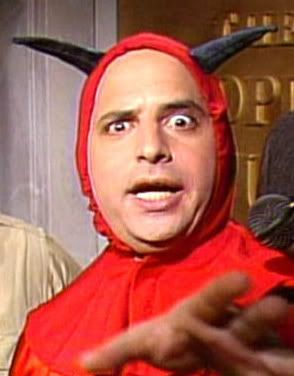
\includegraphics[width=0.5\textwidth]{Images/devil.jpg}
    }
    \vfill
  \end{frame}
}

\AtBeginSubsection[]{
  \begin{frame}
    \vfill
    \centering
    \begin{beamercolorbox}[sep=8pt,center,shadow=true,rounded=true]{title}
    \usebeamerfont{title}\insertsectionhead\par%
    \usebeamerfont{subtitle}\insertsubsectionhead\par%
    \end{beamercolorbox}
    \vfill
  \end{frame}
}
\begin{document}

\title{Welcome to Quarantine General Trivia!\vspace{-0.5in}}
\date{}

\begin{frame}
\titlepage{}
\end{frame}

\begin{frame}
In order to keep Ellen from hearing us put together the questions, we used advanced
technology\ldots
\vspace{1em}
\pause{}
\begin{center}
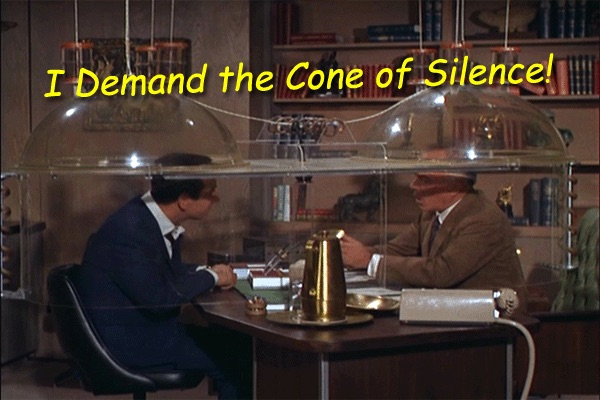
\includegraphics[max width=0.9\textwidth,max height=0.8\textheight]{Images/cone.jpg}
\end{center}
\end{frame}

\begingroup{}
\begin{frame}
\vfill{}
\begin{beamercolorbox}[sep=8pt,center,shadow=true,rounded=true]{title}
\usebeamerfont{title}Good luck everyone! And have fun!
\end{beamercolorbox}
\vfill{}
\end{frame}
\endgroup{}
    

\def\thisSectionName{Sports}
\section{Round 1}
    

\subsection*{Q1}
\begin{frame}[t]{Round 1, Question 1}
\vspace{0.5em}
\begin{block}{Question}
What do you call it when a player makes three back to back strikes in bowling?
\end{block}
\end{frame}
    

\subsection*{Q2}
\begin{frame}[t]{Round 1, Question 2}
\vspace{0.5em}
\begin{block}{Question}
What professional boxer had the most knockouts over his career?
\end{block}
\end{frame}
    

\subsection*{Q3}
\begin{frame}[t]{Round 1, Question 3}
\vspace{0.5em}
\begin{block}{Question}
What is the only country to have played in every single soccer World Cup?
\end{block}
\end{frame}
    

\subsection*{Q4}
\begin{frame}[t]{Round 1, Question 4}
\vspace{0.5em}
\begin{block}{Question}
Wilt Chamberlain holds the record for most points scored by one player in an NBA game. How many points did he score in that game?
\end{block}
\end{frame}
    

\subsection*{Q5}
\begin{frame}[t]{Round 1, Question 5}
\vspace{0.5em}
\begin{block}{Question}
Who was the first person to break the four-minute mile?
\end{block}
\end{frame}
    

\subsection*{Q6}
\begin{frame}[t]{Round 1, Question 6}
\vspace{0.5em}
\begin{block}{Question}
How many championships did the Chicago Bulls win with Michael Jordan on their team?
\end{block}
\end{frame}
    

\subsection*{Q7}
\begin{frame}[t]{Round 1, Question 7}
\vspace{0.5em}
\begin{block}{Question}
The terms ``stale fish'' and ``mulekick'' are commonly used in what sport?
\end{block}
\end{frame}
    

\subsection*{Q8}
\begin{frame}[t]{Round 1, Question 8}
\vspace{0.5em}
\begin{block}{Question}
In the 1900 Olympics, women were allowed to compete for the first time, but in only two sports. Name one of the sports.
\end{block}
\end{frame}
    

\subsection*{Q9}
\begin{frame}[t]{Round 1, Question 9}
\vspace{0.5em}
\begin{block}{Question}
Which sporting event is held every year on Memorial Day?
\end{block}
\end{frame}
    

\subsection*{Q10}
\begin{frame}[t]{Round 1, Question 10}
\vspace{0.5em}
\begin{block}{Question}
All NFL teams have their logo on their helmets, but only one team has the logo on only one side of their helmets. Which team is that?
\end{block}
\end{frame}
    
\subsection{Answers}

\begin{frame}[t]{Round 1, Answer 1}
\vspace{0.5em}
\begin{block}{Question}
What do you call it when a player makes three back to back strikes in bowling?
\end{block}
\visible<2->{
    \begin{block}{Answer}
    A turkey
    \end{block}
}
\end{frame}
    

\begin{frame}[t]{Round 1, Answer 2}
\vspace{0.5em}
\begin{block}{Question}
What professional boxer had the most knockouts over his career?
\end{block}
\visible<2->{
    \begin{columns}[T,totalwidth=\linewidth]
    \begin{column}{0.35\linewidth}
    \begin{block}{Answer}
    Archie Moore
    \end{block}
    \end{column}
    \begin{column}{0.6\linewidth}
    \begin{center}
    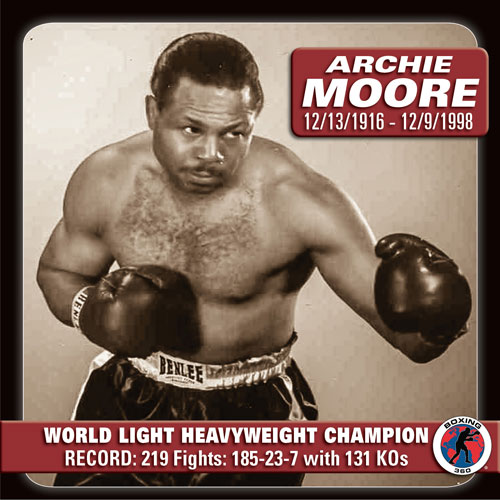
\includegraphics[max width=0.9\textwidth,max height=0.4\textheight]{{Images/archiemoore}.jpg}
    \end{center}
    \end{column}
    \end{columns}
}
\end{frame}
    

\begin{frame}[t]{Round 1, Answer 3}
\vspace{0.5em}
\begin{block}{Question}
What is the only country to have played in every single soccer World Cup?
\end{block}
\visible<2->{
    \begin{block}{Answer}
    Brazil
    \end{block}
}
\end{frame}
    

\begin{frame}[t]{Round 1, Answer 4}
\vspace{0.5em}
\begin{block}{Question}
Wilt Chamberlain holds the record for most points scored by one player in an NBA game. How many points did he score in that game?
\end{block}
\visible<2->{
    \begin{columns}[T,totalwidth=\linewidth]
    \begin{column}{0.35\linewidth}
    \begin{block}{Answer}
    100
    \end{block}
    \end{column}
    \begin{column}{0.6\linewidth}
    \begin{center}
    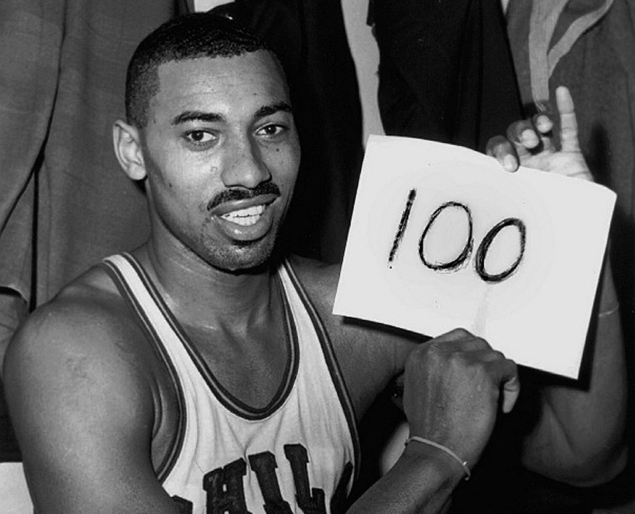
\includegraphics[max width=0.9\textwidth,max height=0.4\textheight]{{Images/wilt}.jpg}
    \end{center}
    \end{column}
    \end{columns}
}
\end{frame}
    

\begin{frame}[t]{Round 1, Answer 5}
\vspace{0.5em}
\begin{block}{Question}
Who was the first person to break the four-minute mile?
\end{block}
\visible<2->{
    \begin{columns}[T,totalwidth=\linewidth]
    \begin{column}{0.35\linewidth}
    \begin{block}{Answer}
    Roger Bannister
    \end{block}
    \end{column}
    \begin{column}{0.6\linewidth}
    \begin{center}
    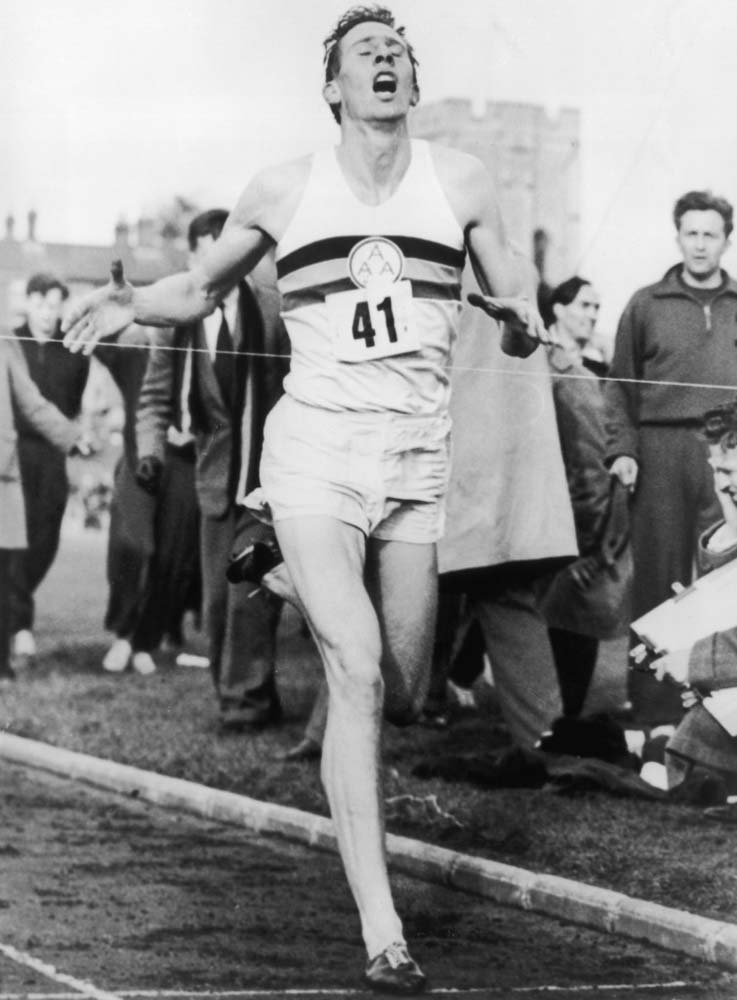
\includegraphics[max width=0.9\textwidth,max height=0.4\textheight]{{Images/Roger-Bannister}.jpg}
    \end{center}
    \end{column}
    \end{columns}
}
\end{frame}
    

\begin{frame}[t]{Round 1, Answer 6}
\vspace{0.5em}
\begin{block}{Question}
How many championships did the Chicago Bulls win with Michael Jordan on their team?
\end{block}
\visible<2->{
    \begin{columns}[T,totalwidth=\linewidth]
    \begin{column}{0.35\linewidth}
    \begin{block}{Answer}
    Six
    \end{block}
    \end{column}
    \begin{column}{0.6\linewidth}
    \begin{center}
    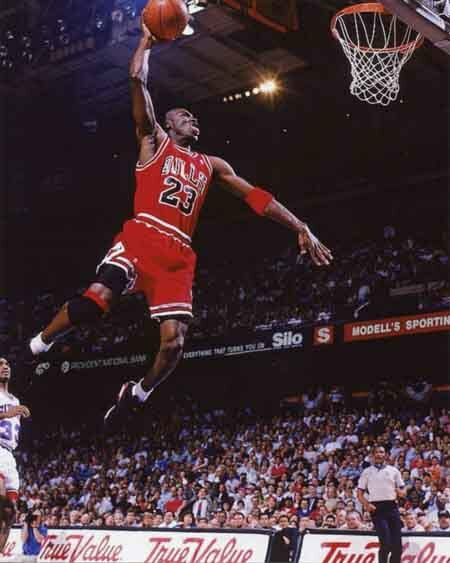
\includegraphics[max width=0.9\textwidth,max height=0.4\textheight]{{Images/michaeljordan}.jpg}
    \end{center}
    \end{column}
    \end{columns}
}
\end{frame}
    

\begin{frame}[t]{Round 1, Answer 7}
\vspace{0.5em}
\begin{block}{Question}
The terms ``stale fish'' and ``mulekick'' are commonly used in what sport?
\end{block}
\visible<2->{
    \begin{columns}[T,totalwidth=\linewidth]
    \begin{column}{0.35\linewidth}
    \begin{block}{Answer}
    Snowboarding
    \end{block}
    \end{column}
    \begin{column}{0.6\linewidth}
    \begin{center}
    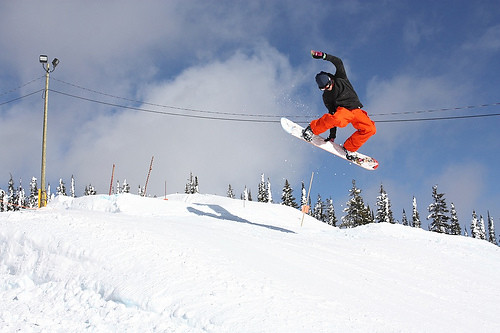
\includegraphics[max width=0.9\textwidth,max height=0.4\textheight]{{Images/stalefish}.jpg}
    \end{center}
    \end{column}
    \end{columns}
}
\end{frame}
    

\begin{frame}[t]{Round 1, Answer 8}
\vspace{0.5em}
\begin{block}{Question}
In the 1900 Olympics, women were allowed to compete for the first time, but in only two sports. Name one of the sports.
\end{block}
\visible<2->{
    \begin{columns}[T,totalwidth=\linewidth]
    \begin{column}{0.35\linewidth}
    \begin{block}{Answer}
    Tennis and golf
    \end{block}
    \end{column}
    \begin{column}{0.6\linewidth}
    \begin{center}
    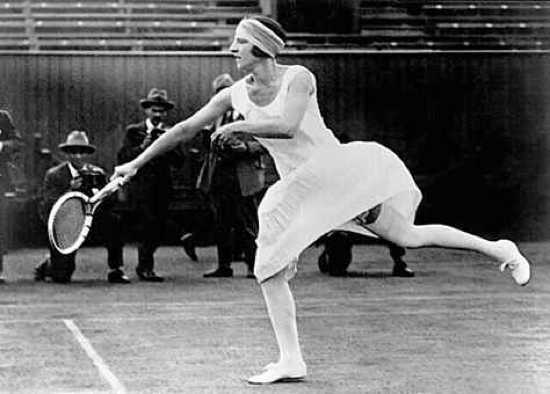
\includegraphics[max width=0.9\textwidth,max height=0.4\textheight]{{Images/womentennis}.jpg}
    \end{center}
    \end{column}
    \end{columns}
}
\end{frame}
    

\begin{frame}[t]{Round 1, Answer 9}
\vspace{0.5em}
\begin{block}{Question}
Which sporting event is held every year on Memorial Day?
\end{block}
\visible<2->{
    \begin{columns}[T,totalwidth=\linewidth]
    \begin{column}{0.35\linewidth}
    \begin{block}{Answer}
    The Indianapolis 500
    \end{block}
    \end{column}
    \begin{column}{0.6\linewidth}
    \begin{center}
    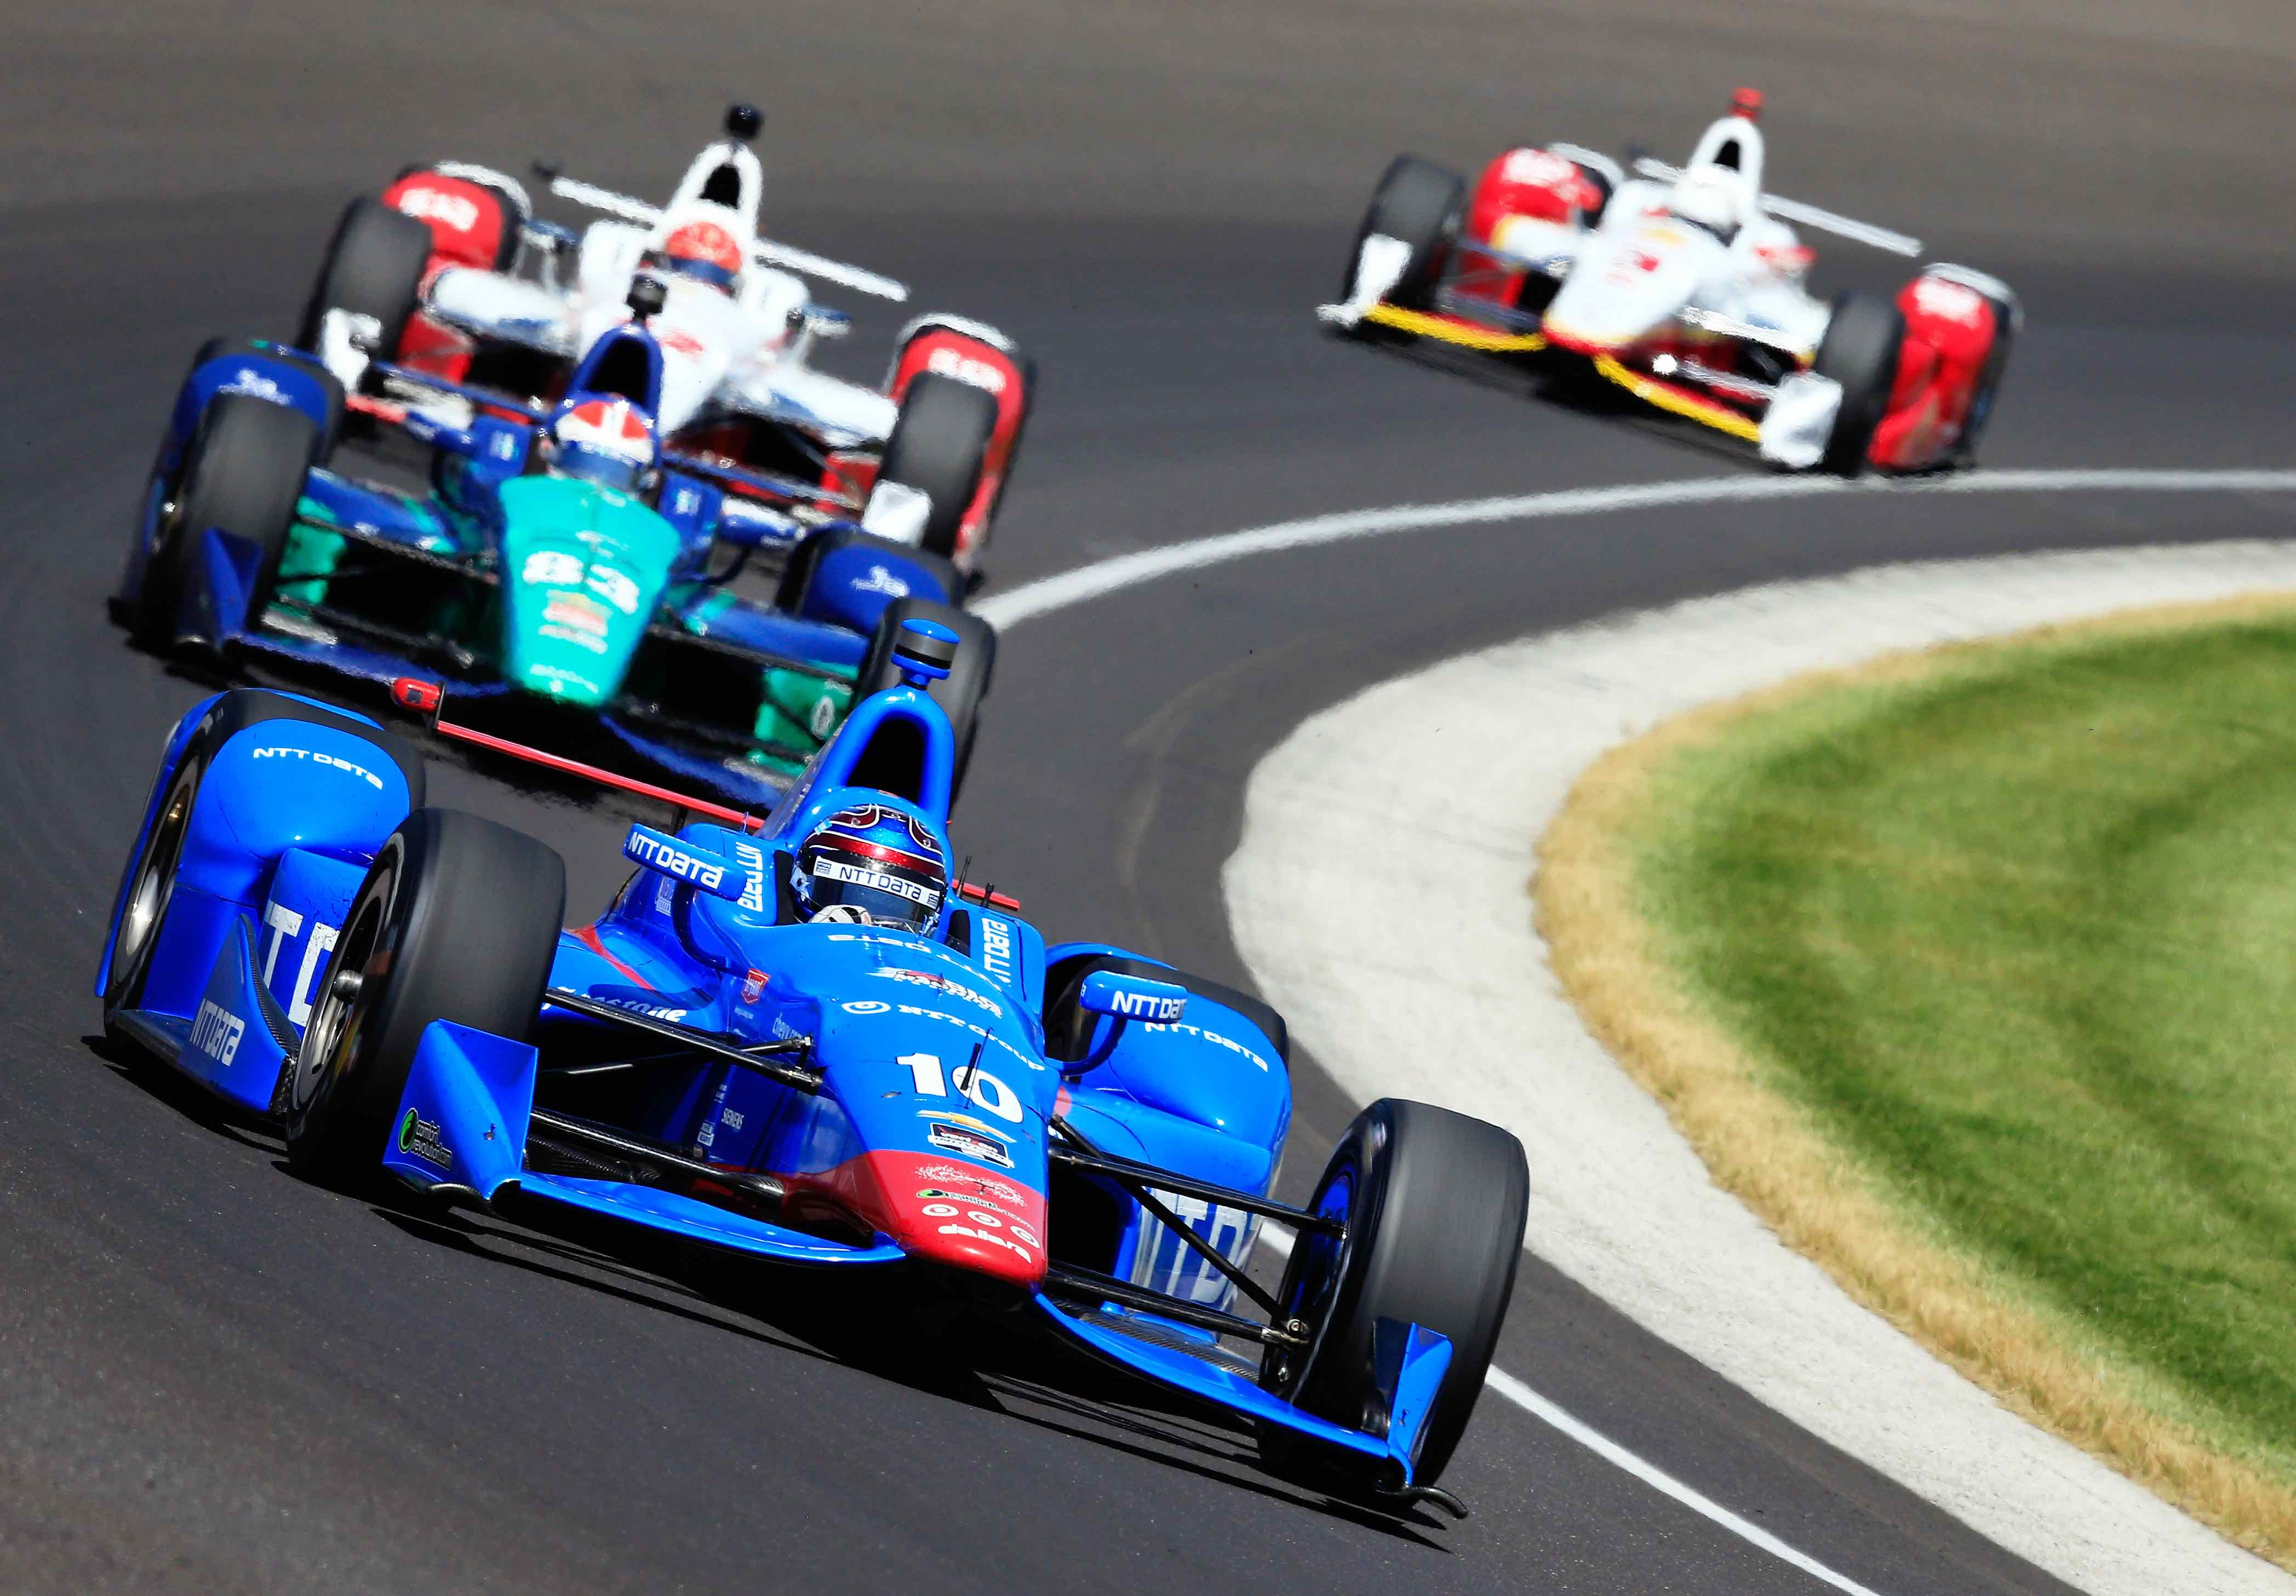
\includegraphics[max width=0.9\textwidth,max height=0.4\textheight]{{Images/indy500}.jpg}
    \end{center}
    \end{column}
    \end{columns}
}
\end{frame}
    

\begin{frame}[t]{Round 1, Answer 10}
\vspace{0.5em}
\begin{block}{Question}
All NFL teams have their logo on their helmets, but only one team has the logo on only one side of their helmets. Which team is that?
\end{block}
\visible<2->{
    \begin{columns}[T,totalwidth=\linewidth]
    \begin{column}{0.35\linewidth}
    \begin{block}{Answer}
    The Steelers (it's on the right side)
    \end{block}
    \end{column}
    \begin{column}{0.6\linewidth}
    \begin{center}
    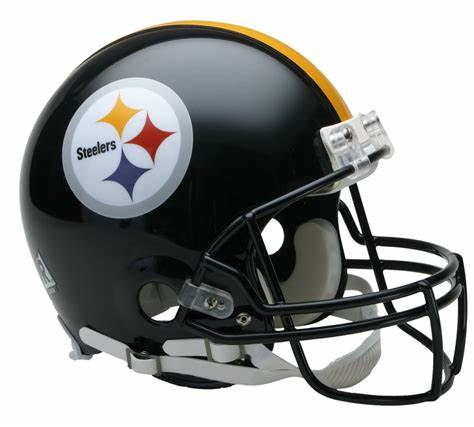
\includegraphics[max width=0.9\textwidth,max height=0.4\textheight]{{Images/steelers}.jpeg}
    \end{center}
    \end{column}
    \end{columns}
}
\end{frame}
    

\def\thisSectionName{Plays and Playwrights}
\section{Round 2}
    

\subsection*{Q1}
\begin{frame}[t]{Round 2, Question 1}
\vspace{0.5em}
\begin{block}{Question}
Who wrote \emph{The Importance of being Earnest?}
\end{block}
\end{frame}
    

\subsection*{Q2}
\begin{frame}[t]{Round 2, Question 2}
\vspace{0.5em}
\begin{block}{Question}
What Thornton Wilder play became the musical \emph{Hello Dolly}? (The play has two names --- we will take either one.)
\end{block}
\end{frame}
    

\subsection*{Q3}
\begin{frame}[t]{Round 2, Question 3}
\vspace{0.5em}
\begin{block}{Question}
``We are such stuff as dreams are made on.'' What Shakespeare play is this line from?
\end{block}
\end{frame}
    

\subsection*{Q4}
\begin{frame}[t]{Round 2, Question 4}
\vspace{0.5em}
\begin{block}{Question}
``We are such things as rubbish is made of, so let's drink up and forget it.'' What famous American play is this line from?
\end{block}
\end{frame}
    

\subsection*{Q5}
\begin{frame}[t]{Round 2, Question 5}
\vspace{0.5em}
\begin{block}{Question}
Name the ancient Greek playwright who wrote \emph{The Frogs}.
\end{block}
\end{frame}
    

\subsection*{Q6}
\begin{frame}[t]{Round 2, Question 6}
\vspace{0.5em}
\begin{block}{Question}
Which Off-Broadway play that opened in 1960 ran for so long that \emph{The New Yorker} started to run a serialization of Joyce's \emph{Ulysses} in its ``Goings On About Town'' column instead of the usual synopsis of the play?
\end{block}
\end{frame}
    

\subsection*{Q7}
\begin{frame}[t]{Round 2, Question 7}
\vspace{0.5em}
\begin{block}{Question}
Who wrote the play upon which the musical \emph{My Fair Lady} was based?
\end{block}
\end{frame}
    

\subsection*{Q8}
\begin{frame}[t]{Round 2, Question 8}
\vspace{0.5em}
\begin{block}{Question}
To which famous movie star was Arthur Miller married? 
\end{block}
\end{frame}
    

\subsection*{Q9}
\begin{frame}[t]{Round 2, Question 9}
\vspace{0.5em}
\begin{block}{Question}
Which French comedic playwright wrote \emph{Tartuffe}, \emph{The School for Wives}, \emph{The Miser}, and \emph{The Hypochondriac}\,?
\end{block}
\end{frame}
    

\subsection*{Q10}
\begin{frame}[t]{Round 2, Question 10}
\vspace{0.5em}
\begin{block}{Question}
Who wrote \emph{Angels in America}\,?
\end{block}
\end{frame}
    
\subsection{Answers}

\begin{frame}[t]{Round 2, Answer 1}
\vspace{0.5em}
\begin{block}{Question}
Who wrote \emph{The Importance of being Earnest?}
\end{block}
\visible<2->{
    \begin{columns}[T,totalwidth=\linewidth]
    \begin{column}{0.35\linewidth}
    \begin{block}{Answer}
    Oscar Wilde
    \end{block}
    \end{column}
    \begin{column}{0.6\linewidth}
    \begin{center}
    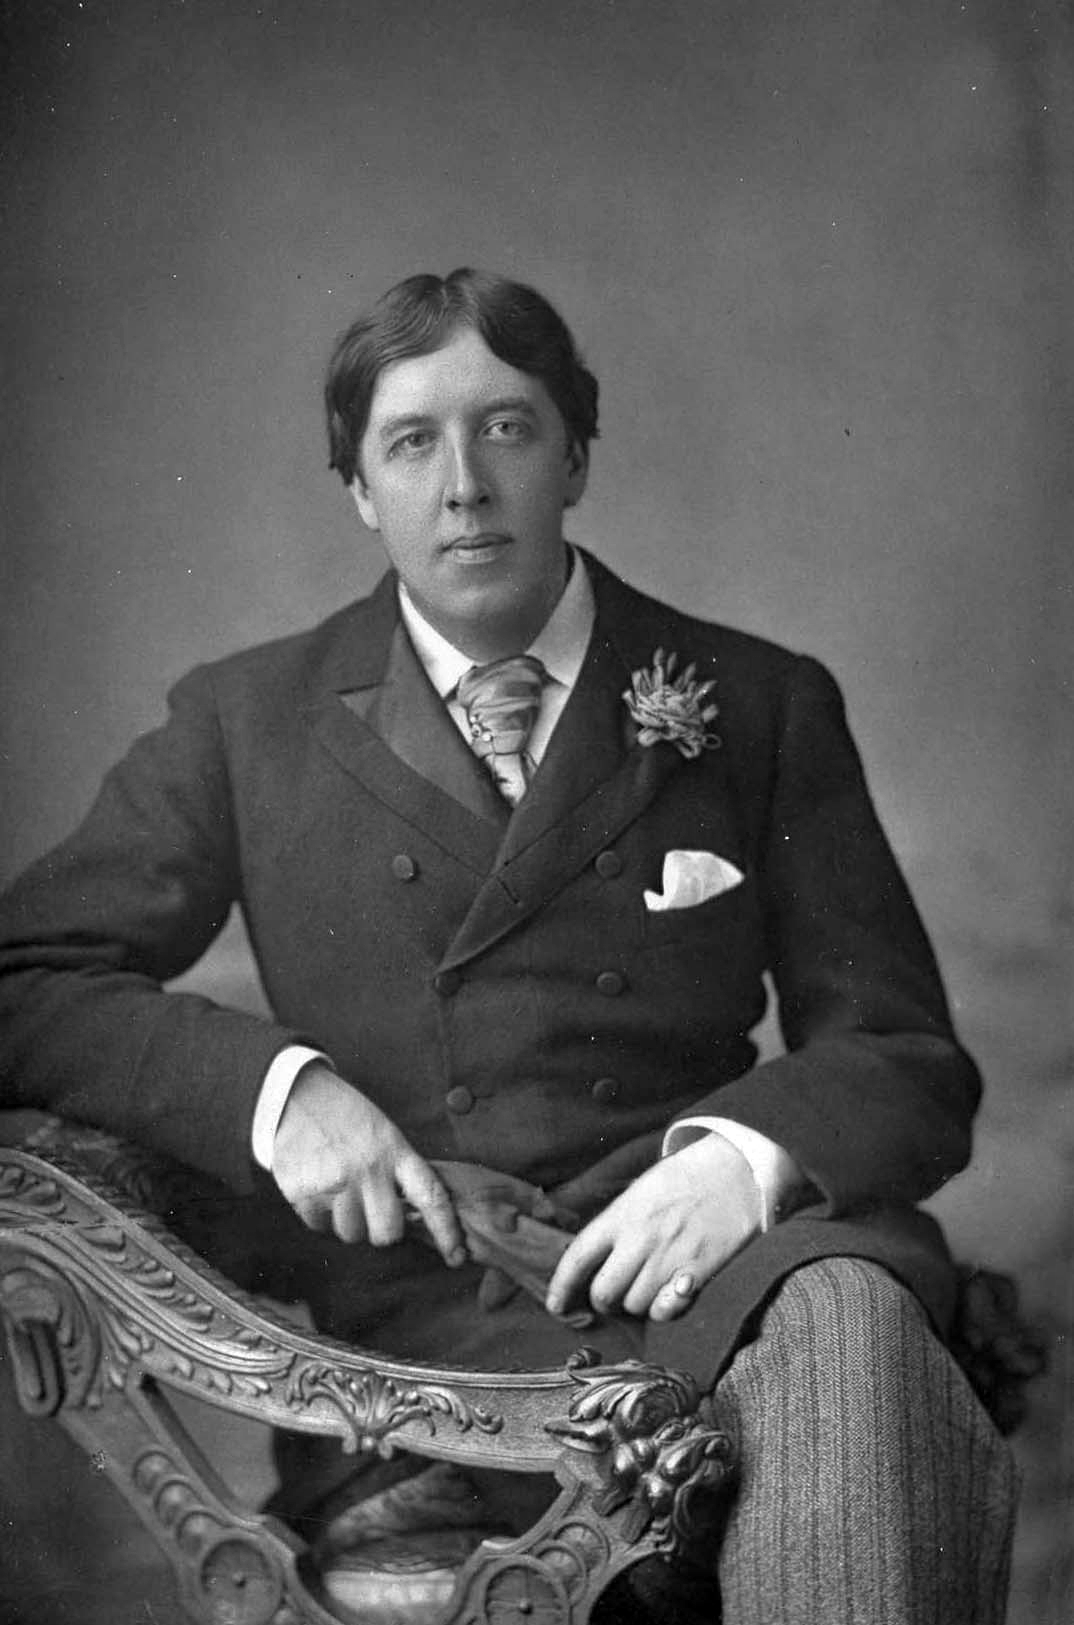
\includegraphics[max width=0.9\textwidth,max height=0.4\textheight]{{Images/oscarwilde}.jpg}
    \end{center}
    \end{column}
    \end{columns}
}
\end{frame}
    

\begin{frame}[t]{Round 2, Answer 2}
\vspace{0.5em}
\begin{block}{Question}
What Thornton Wilder play became the musical \emph{Hello Dolly}? (The play has two names --- we will take either one.)
\end{block}
\visible<2->{
    \begin{columns}[T,totalwidth=\linewidth]
    \begin{column}{0.35\linewidth}
    \begin{block}{Answer}
     \emph{The Merchant of Yonkers} or \emph{The Matchmaker}.
    \end{block}
    \end{column}
    \begin{column}{0.6\linewidth}
    \begin{center}
    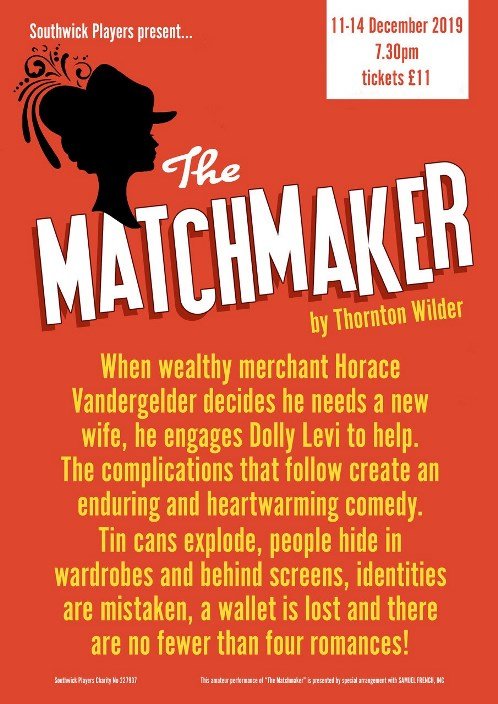
\includegraphics[max width=0.9\textwidth,max height=0.4\textheight]{{Images/matchmaker}.jpg}
    \end{center}
    \end{column}
    \end{columns}
}
\end{frame}
    

\begin{frame}[t]{Round 2, Answer 3}
\vspace{0.5em}
\begin{block}{Question}
``We are such stuff as dreams are made on.'' What Shakespeare play is this line from?
\end{block}
\visible<2->{
    \begin{columns}[T,totalwidth=\linewidth]
    \begin{column}{0.35\linewidth}
    \begin{block}{Answer}
    \emph{The Tempest}
    \end{block}
    \end{column}
    \begin{column}{0.6\linewidth}
    \begin{center}
    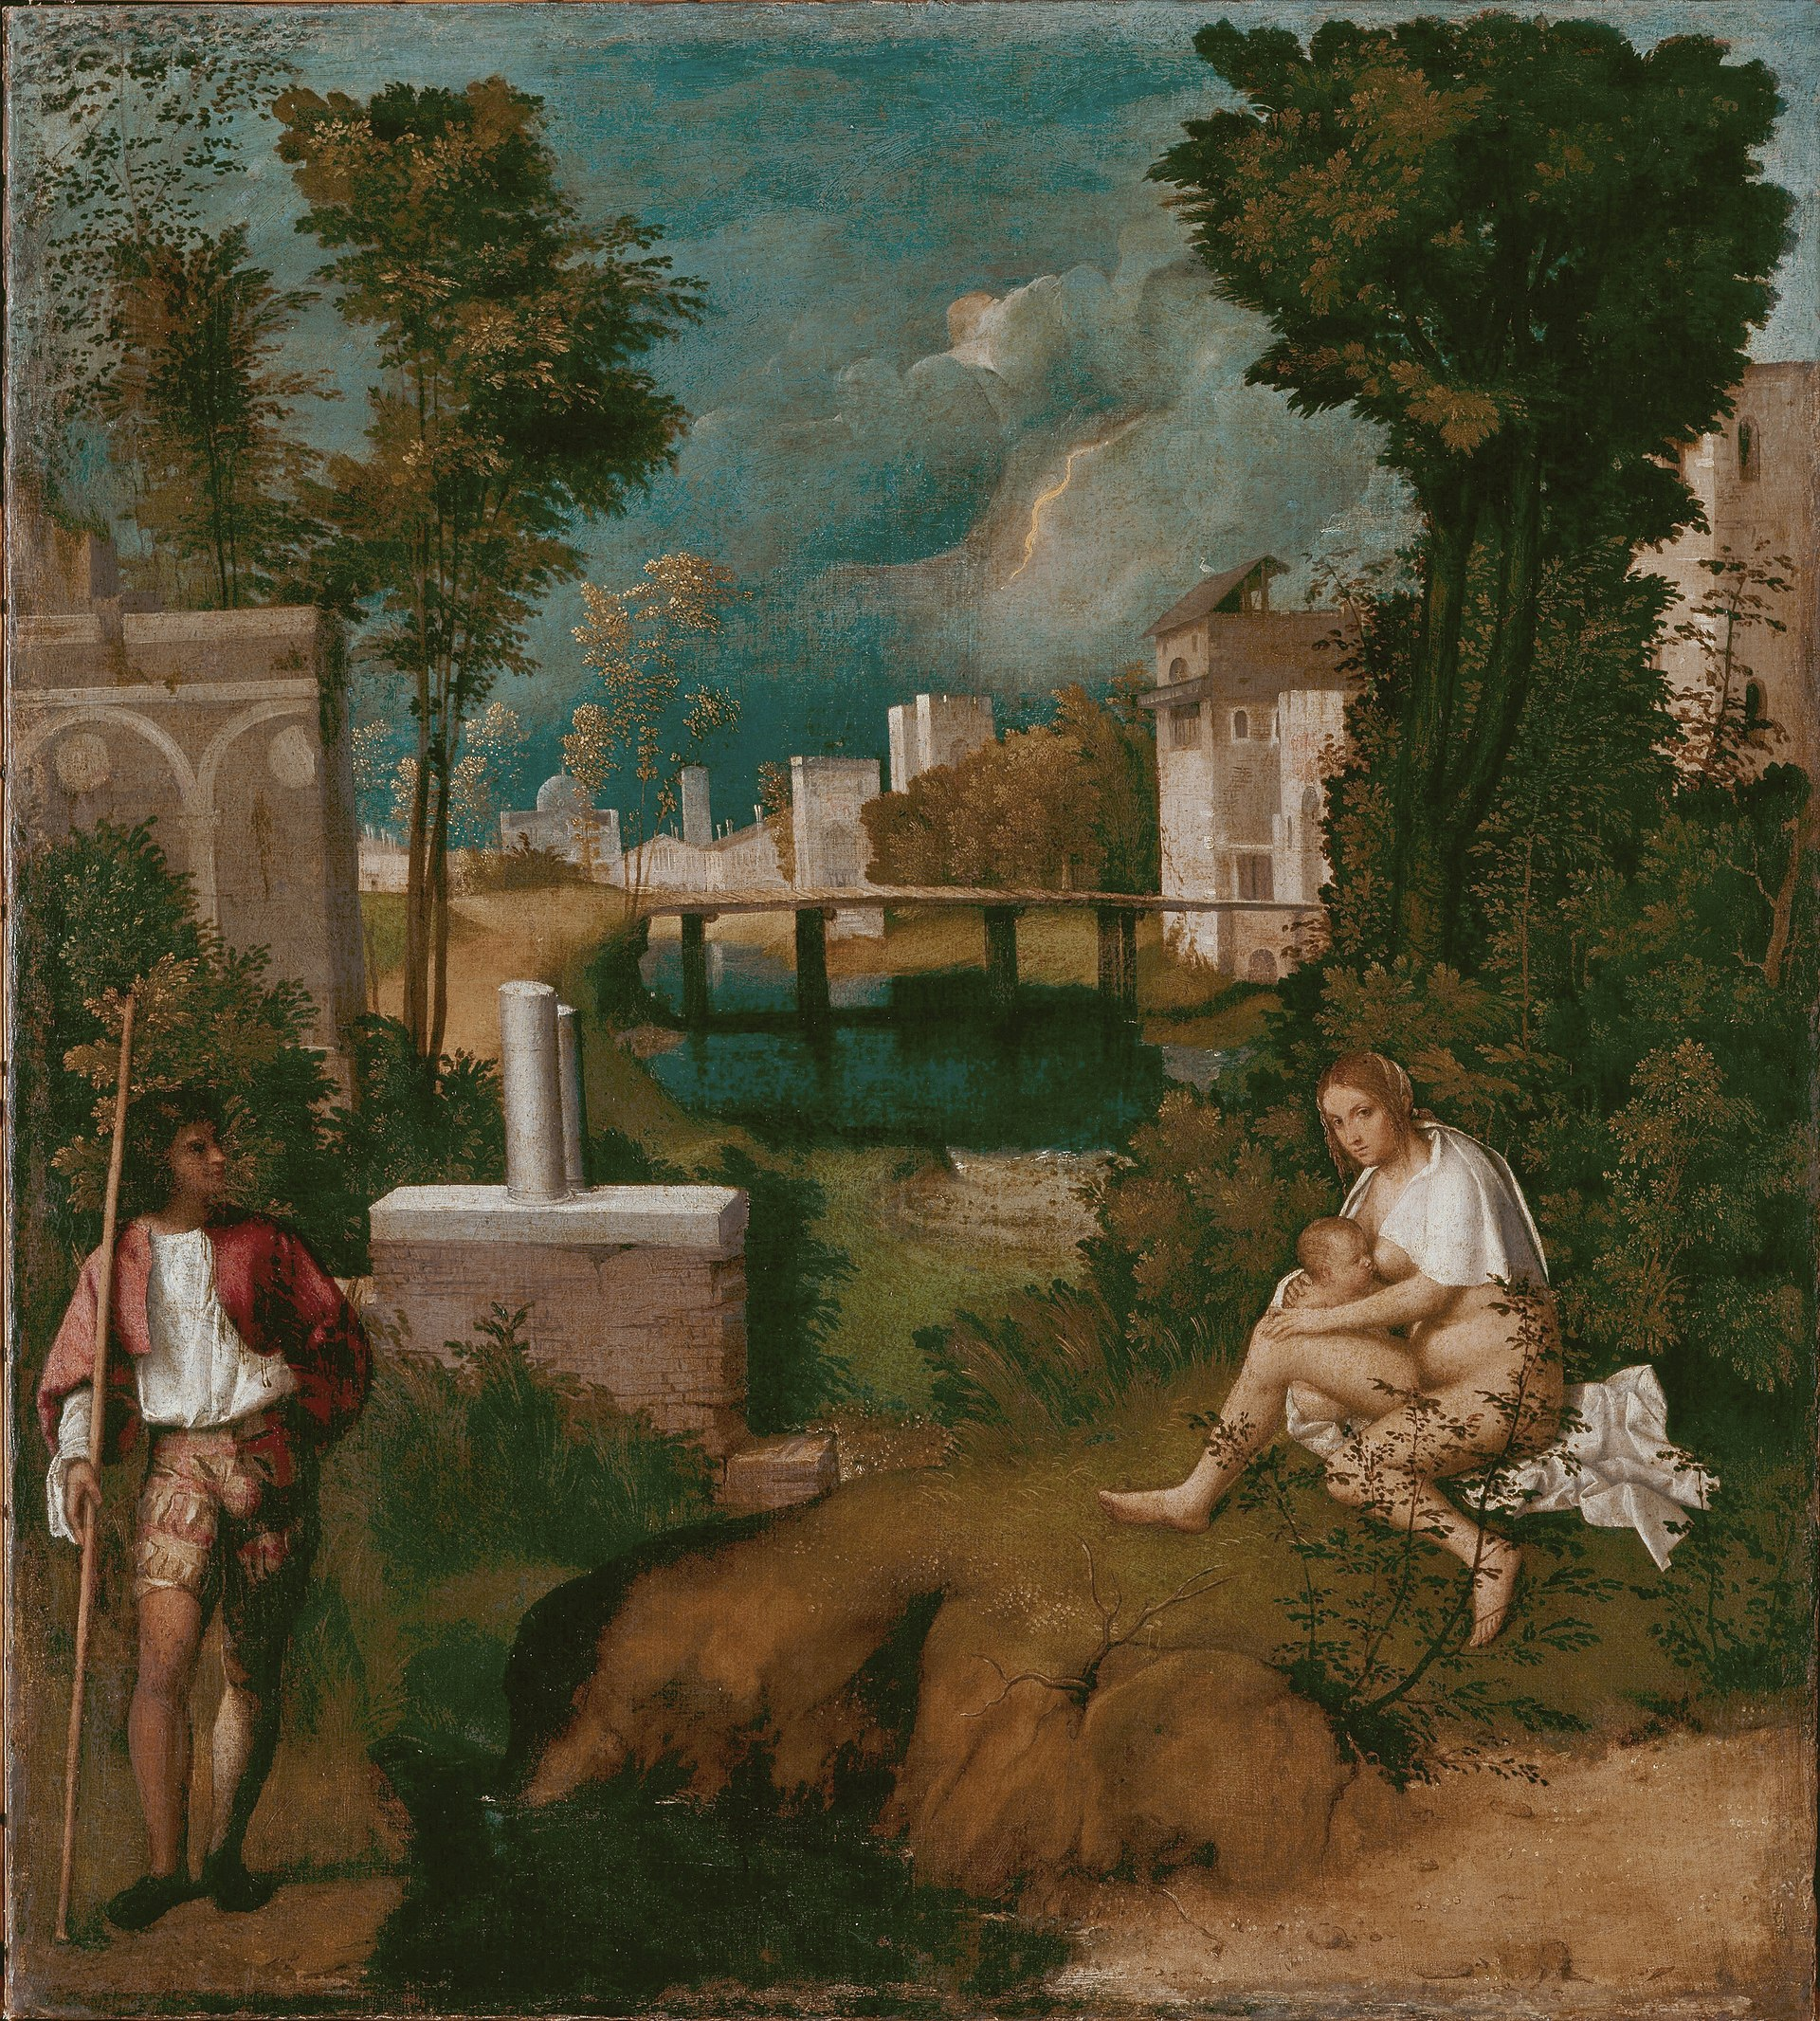
\includegraphics[max width=0.9\textwidth,max height=0.4\textheight]{{Images/tempest}.jpg}
    \end{center}
    \end{column}
    \end{columns}
}
\end{frame}
    

\begin{frame}[t]{Round 2, Answer 4}
\vspace{0.5em}
\begin{block}{Question}
``We are such things as rubbish is made of, so let's drink up and forget it.'' What famous American play is this line from?
\end{block}
\visible<2->{
    \begin{block}{Answer}
    \emph{Long Day's Journey into Night}
    \end{block}
}
\end{frame}
    

\begin{frame}[t]{Round 2, Answer 5}
\vspace{0.5em}
\begin{block}{Question}
Name the ancient Greek playwright who wrote \emph{The Frogs}.
\end{block}
\visible<2->{
    \begin{block}{Answer}
    Aristophanes
    \end{block}
}
\end{frame}
    

\begin{frame}[t]{Round 2, Answer 6}
\vspace{0.5em}
\begin{block}{Question}
Which Off-Broadway play that opened in 1960 ran for so long that \emph{The New Yorker} started to run a serialization of Joyce's \emph{Ulysses} in its ``Goings On About Town'' column instead of the usual synopsis of the play?
\end{block}
\visible<2->{
    \begin{columns}[T,totalwidth=\linewidth]
    \begin{column}{0.35\linewidth}
    \begin{block}{Answer}
    The Fantasticks
    \end{block}
    \end{column}
    \begin{column}{0.6\linewidth}
    \begin{center}
    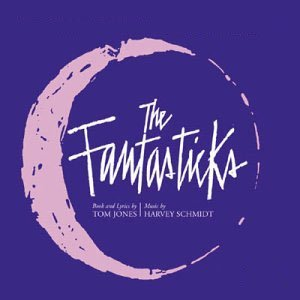
\includegraphics[max width=0.9\textwidth,max height=0.4\textheight]{{Images/fantasticks}.jpg}
    \end{center}
    \end{column}
    \end{columns}
}
\end{frame}
    

\begin{frame}[t]{Round 2, Answer 7}
\vspace{0.5em}
\begin{block}{Question}
Who wrote the play upon which the musical \emph{My Fair Lady} was based?
\end{block}
\visible<2->{
    \begin{columns}[T,totalwidth=\linewidth]
    \begin{column}{0.35\linewidth}
    \begin{block}{Answer}
    George Bernard Shaw (\emph{Pygmalion})
    \end{block}
    \end{column}
    \begin{column}{0.6\linewidth}
    \begin{center}
    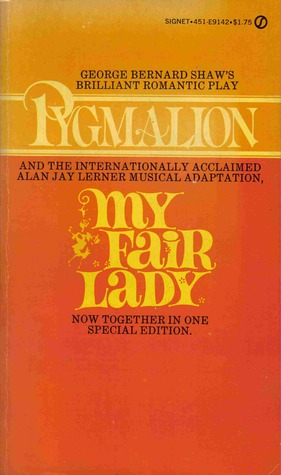
\includegraphics[max width=0.9\textwidth,max height=0.4\textheight]{{Images/pygmalion}.jpg}
    \end{center}
    \end{column}
    \end{columns}
}
\end{frame}
    

\begin{frame}[t]{Round 2, Answer 8}
\vspace{0.5em}
\begin{block}{Question}
To which famous movie star was Arthur Miller married? 
\end{block}
\visible<2->{
    \begin{columns}[T,totalwidth=\linewidth]
    \begin{column}{0.35\linewidth}
    \begin{block}{Answer}
    Marilyn Monroe
    \end{block}
    \end{column}
    \begin{column}{0.6\linewidth}
    \begin{center}
    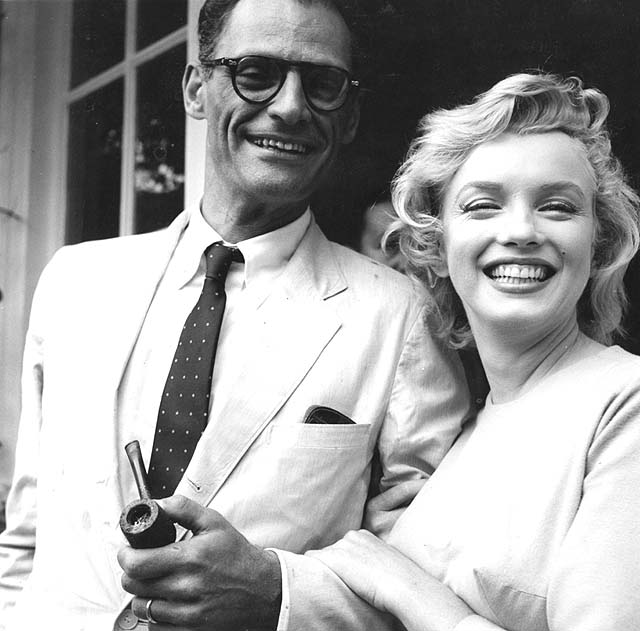
\includegraphics[max width=0.9\textwidth,max height=0.4\textheight]{{Images/Arthur-Miller-Marilyn-Monroe}.jpg}
    \end{center}
    \end{column}
    \end{columns}
}
\end{frame}
    

\begin{frame}[t]{Round 2, Answer 9}
\vspace{0.5em}
\begin{block}{Question}
Which French comedic playwright wrote \emph{Tartuffe}, \emph{The School for Wives}, \emph{The Miser}, and \emph{The Hypochondriac}\,?
\end{block}
\visible<2->{
    \begin{block}{Answer}
    Molière
    \end{block}
}
\end{frame}
    

\begin{frame}[t]{Round 2, Answer 10}
\vspace{0.5em}
\begin{block}{Question}
Who wrote \emph{Angels in America}\,?
\end{block}
\visible<2->{
    \begin{columns}[T,totalwidth=\linewidth]
    \begin{column}{0.35\linewidth}
    \begin{block}{Answer}
    Tony Kushner
    \end{block}
    \end{column}
    \begin{column}{0.6\linewidth}
    \begin{center}
    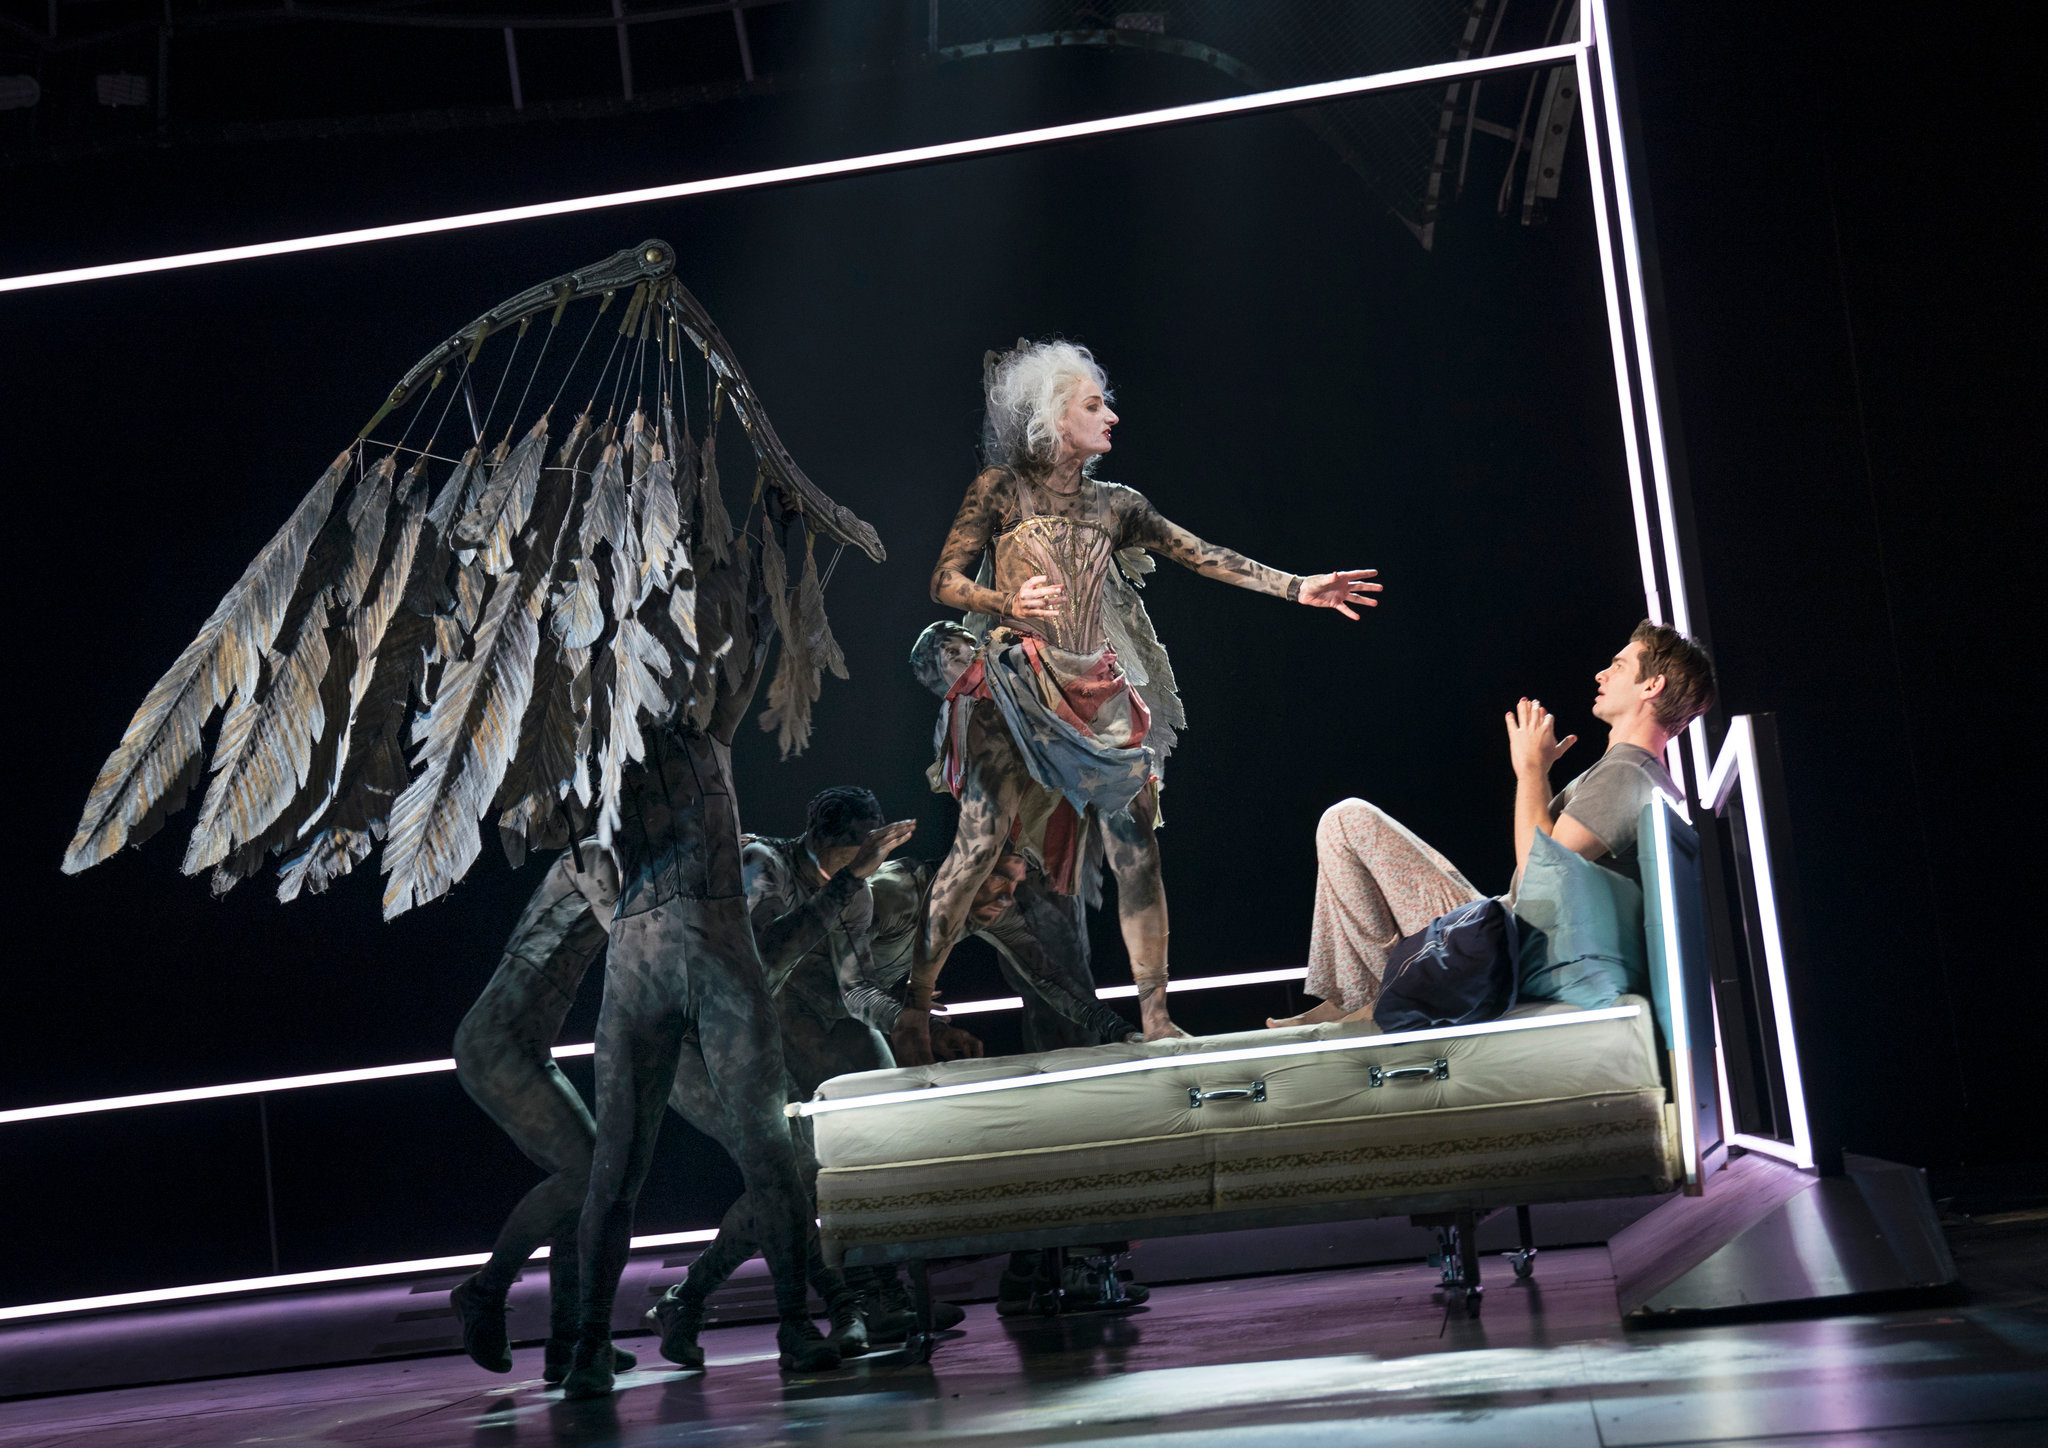
\includegraphics[max width=0.9\textwidth,max height=0.4\textheight]{{Images/angelsinamerica}.jpg}
    \end{center}
    \end{column}
    \end{columns}
}
\end{frame}
    

\def\thisSectionName{Women in American History}
\section{Round 3}
    

\subsection*{Q1}
\begin{frame}[t]{Round 3, Question 1}
\vspace{0.5em}
\begin{block}{Question}
What was Amelia Earhart's ultimate goal in making the trip during which she crashed?
\end{block}
\end{frame}
    

\subsection*{Q2}
\begin{frame}[t]{Round 3, Question 2}
\vspace{0.5em}
\begin{block}{Question}
Who wrote the poem, ``Because I could not stop for Death''?
\end{block}
\end{frame}
    

\subsection*{Q3}
\begin{frame}[t]{Round 3, Question 3}
\vspace{0.5em}
\begin{block}{Question}
Who was the famous translator on the Lewis and Clark expedition?
\end{block}
\end{frame}
    

\subsection*{Q4}
\begin{frame}[t]{Round 3, Question 4}
\vspace{0.5em}
\begin{block}{Question}
Which computer scientist, who was also a US Navy rear admiral, developed one of the first compilers (a program that translates human-readable instructions into computer code)?
\end{block}
\end{frame}
    

\subsection*{Q5}
\begin{frame}[t]{Round 3, Question 5}
\vspace{0.5em}
\begin{block}{Question}
Anne Sullivan is best known from her association with what other famous American woman?
\end{block}
\end{frame}
    

\subsection*{Q6}
\begin{frame}[t]{Round 3, Question 6}
\vspace{0.5em}
\begin{block}{Question}
This woman was the first woman elected to Congress and was one of the few congresspeople to vote against both the World War I and World War II declarations of war.
\end{block}
\end{frame}
    

\subsection*{Q7}
\begin{frame}[t]{Round 3, Question 7}
\vspace{0.5em}
\begin{block}{Question}
Who wrote \emph{Little Women}\,?
\end{block}
\end{frame}
    

\subsection*{Q8}
\begin{frame}[t]{Round 3, Question 8}
\vspace{0.5em}
\begin{block}{Question}
Who designed the Vietnam War Memorial on the Mall in Washington, D.C.?
\end{block}
\end{frame}
    

\subsection*{Q9}
\begin{frame}[t]{Round 3, Question 9}
\vspace{0.5em}
\begin{block}{Question}
Which woman wrote a book about the absence of birdsong that brought attention to the environmental movement?
\end{block}
\end{frame}
    

\subsection*{Q10}
\begin{frame}[t]{Round 3, Question 10}
\vspace{0.5em}
\begin{block}{Question}
Clara Barton founded and served as the first president of what organization?
\end{block}
\end{frame}
    
\subsection{Answers}

\begin{frame}[t]{Round 3, Answer 1}
\vspace{0.5em}
\begin{block}{Question}
What was Amelia Earhart's ultimate goal in making the trip during which she crashed?
\end{block}
\visible<2->{
    \begin{columns}[T,totalwidth=\linewidth]
    \begin{column}{0.35\linewidth}
    \begin{block}{Answer}
    Circumnavigating the globe
    \end{block}
    \end{column}
    \begin{column}{0.6\linewidth}
    \begin{center}
    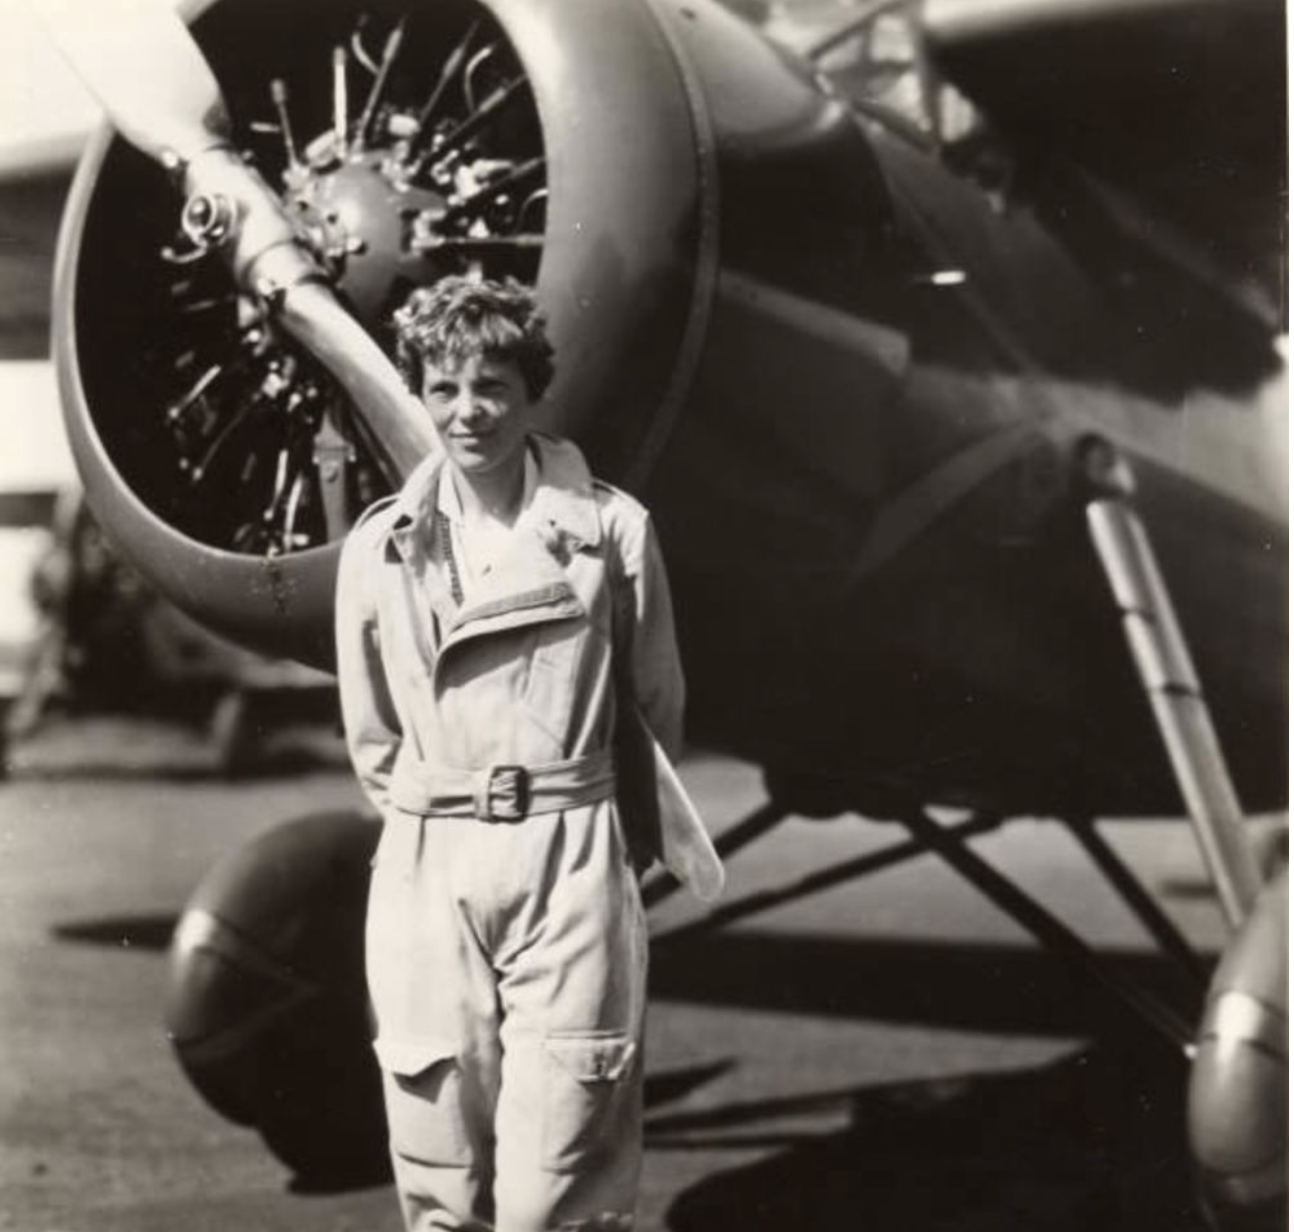
\includegraphics[max width=0.9\textwidth,max height=0.4\textheight]{{Images/earheart}.png}
    \end{center}
    \end{column}
    \end{columns}
}
\end{frame}
    

\begin{frame}[t]{Round 3, Answer 2}
\vspace{0.5em}
\begin{block}{Question}
Who wrote the poem, ``Because I could not stop for Death''?
\end{block}
\visible<2->{
    \begin{columns}[T,totalwidth=\linewidth]
    \begin{column}{0.35\linewidth}
    \begin{block}{Answer}
    Emily Dickinson
    \end{block}
    \end{column}
    \begin{column}{0.6\linewidth}
    \begin{center}
    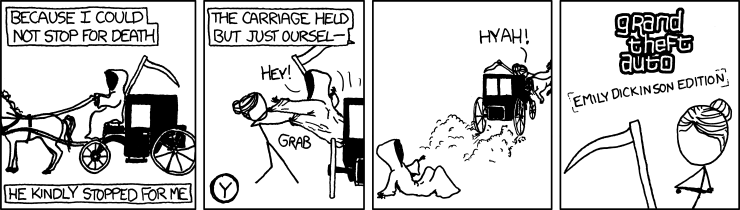
\includegraphics[max width=0.9\textwidth,max height=0.4\textheight]{{Images/xkcddickinson}.png}
    \end{center}
    \end{column}
    \end{columns}
}
\end{frame}
    

\begin{frame}[t]{Round 3, Answer 3}
\vspace{0.5em}
\begin{block}{Question}
Who was the famous translator on the Lewis and Clark expedition?
\end{block}
\visible<2->{
    \begin{columns}[T,totalwidth=\linewidth]
    \begin{column}{0.35\linewidth}
    \begin{block}{Answer}
    Sacagawea
    \end{block}
    \end{column}
    \begin{column}{0.6\linewidth}
    \begin{center}
    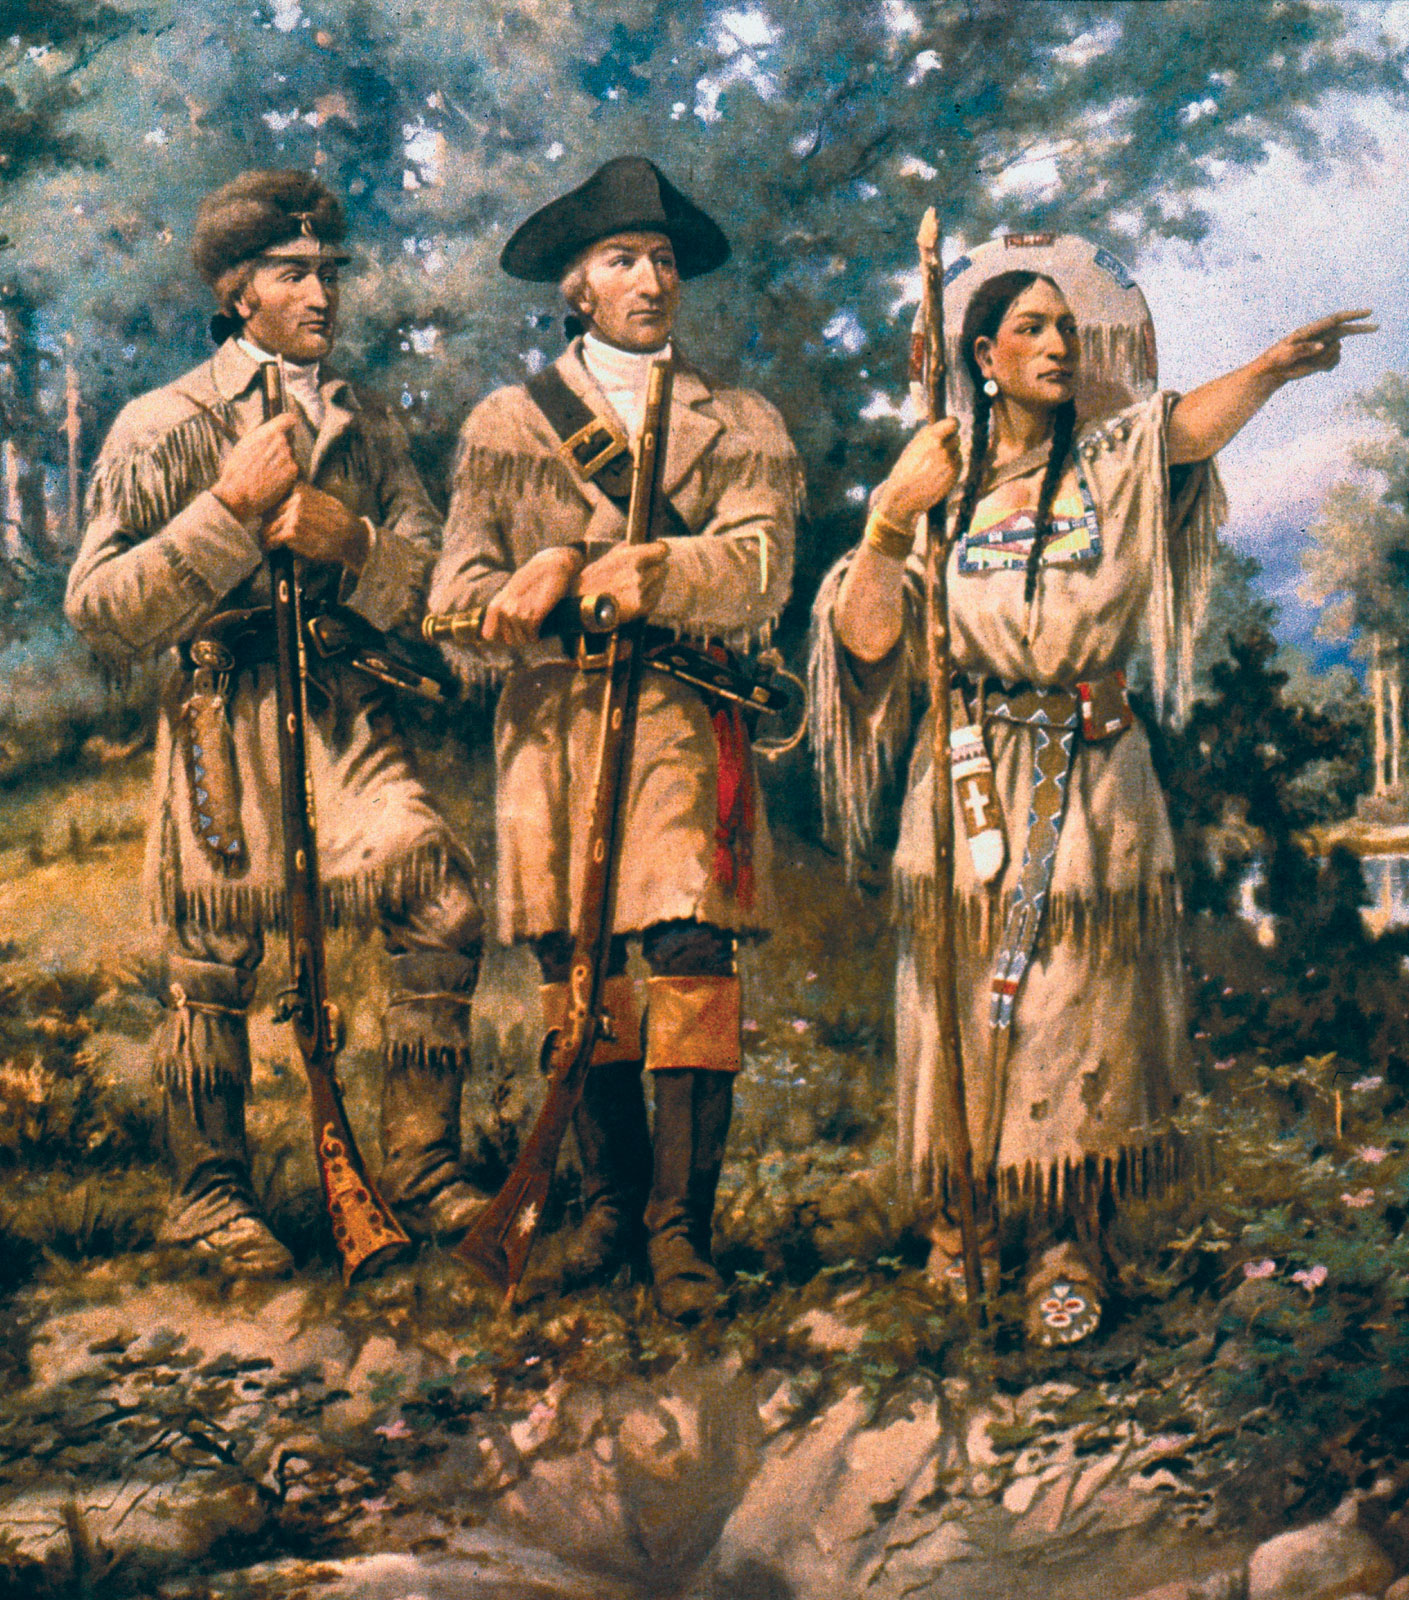
\includegraphics[max width=0.9\textwidth,max height=0.4\textheight]{{Images/sacagawea}.jpg}
    \end{center}
    \end{column}
    \end{columns}
}
\end{frame}
    

\begin{frame}[t]{Round 3, Answer 4}
\vspace{0.5em}
\begin{block}{Question}
Which computer scientist, who was also a US Navy rear admiral, developed one of the first compilers (a program that translates human-readable instructions into computer code)?
\end{block}
\visible<2->{
    \begin{columns}[T,totalwidth=\linewidth]
    \begin{column}{0.35\linewidth}
    \begin{block}{Answer}
    Grace Hopper
    \end{block}
    \end{column}
    \begin{column}{0.6\linewidth}
    \begin{center}
    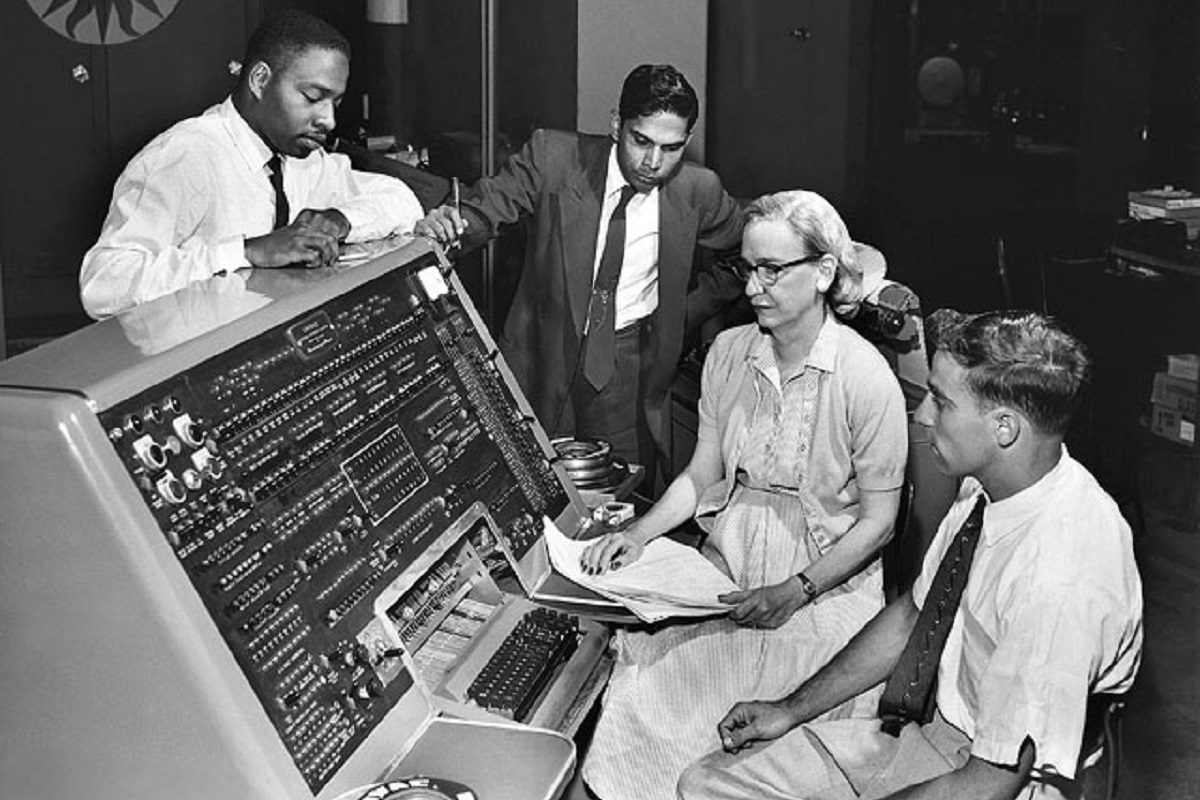
\includegraphics[max width=0.9\textwidth,max height=0.4\textheight]{{Images/hopper}.jpg}
    \end{center}
    \end{column}
    \end{columns}
}
\end{frame}
    

\begin{frame}[t]{Round 3, Answer 5}
\vspace{0.5em}
\begin{block}{Question}
Anne Sullivan is best known from her association with what other famous American woman?
\end{block}
\visible<2->{
    \begin{columns}[T,totalwidth=\linewidth]
    \begin{column}{0.35\linewidth}
    \begin{block}{Answer}
    Hellen Keller (she was Keller's teacher)
    \end{block}
    \end{column}
    \begin{column}{0.6\linewidth}
    \begin{center}
    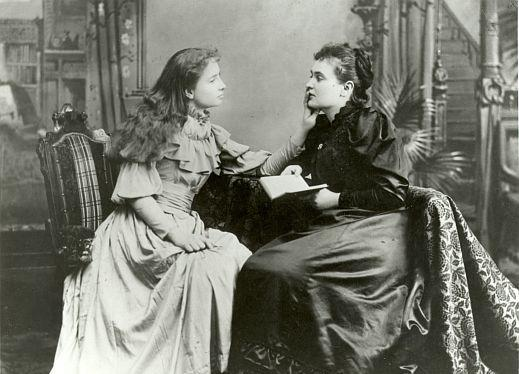
\includegraphics[max width=0.9\textwidth,max height=0.4\textheight]{{Images/helen-and-anne}.jpg}
    \end{center}
    \end{column}
    \end{columns}
}
\end{frame}
    

\begin{frame}[t]{Round 3, Answer 6}
\vspace{0.5em}
\begin{block}{Question}
This woman was the first woman elected to Congress and was one of the few congresspeople to vote against both the World War I and World War II declarations of war.
\end{block}
\visible<2->{
    \begin{columns}[T,totalwidth=\linewidth]
    \begin{column}{0.35\linewidth}
    \begin{block}{Answer}
    Jeanette Rankin
    \end{block}
    \end{column}
    \begin{column}{0.6\linewidth}
    \begin{center}
    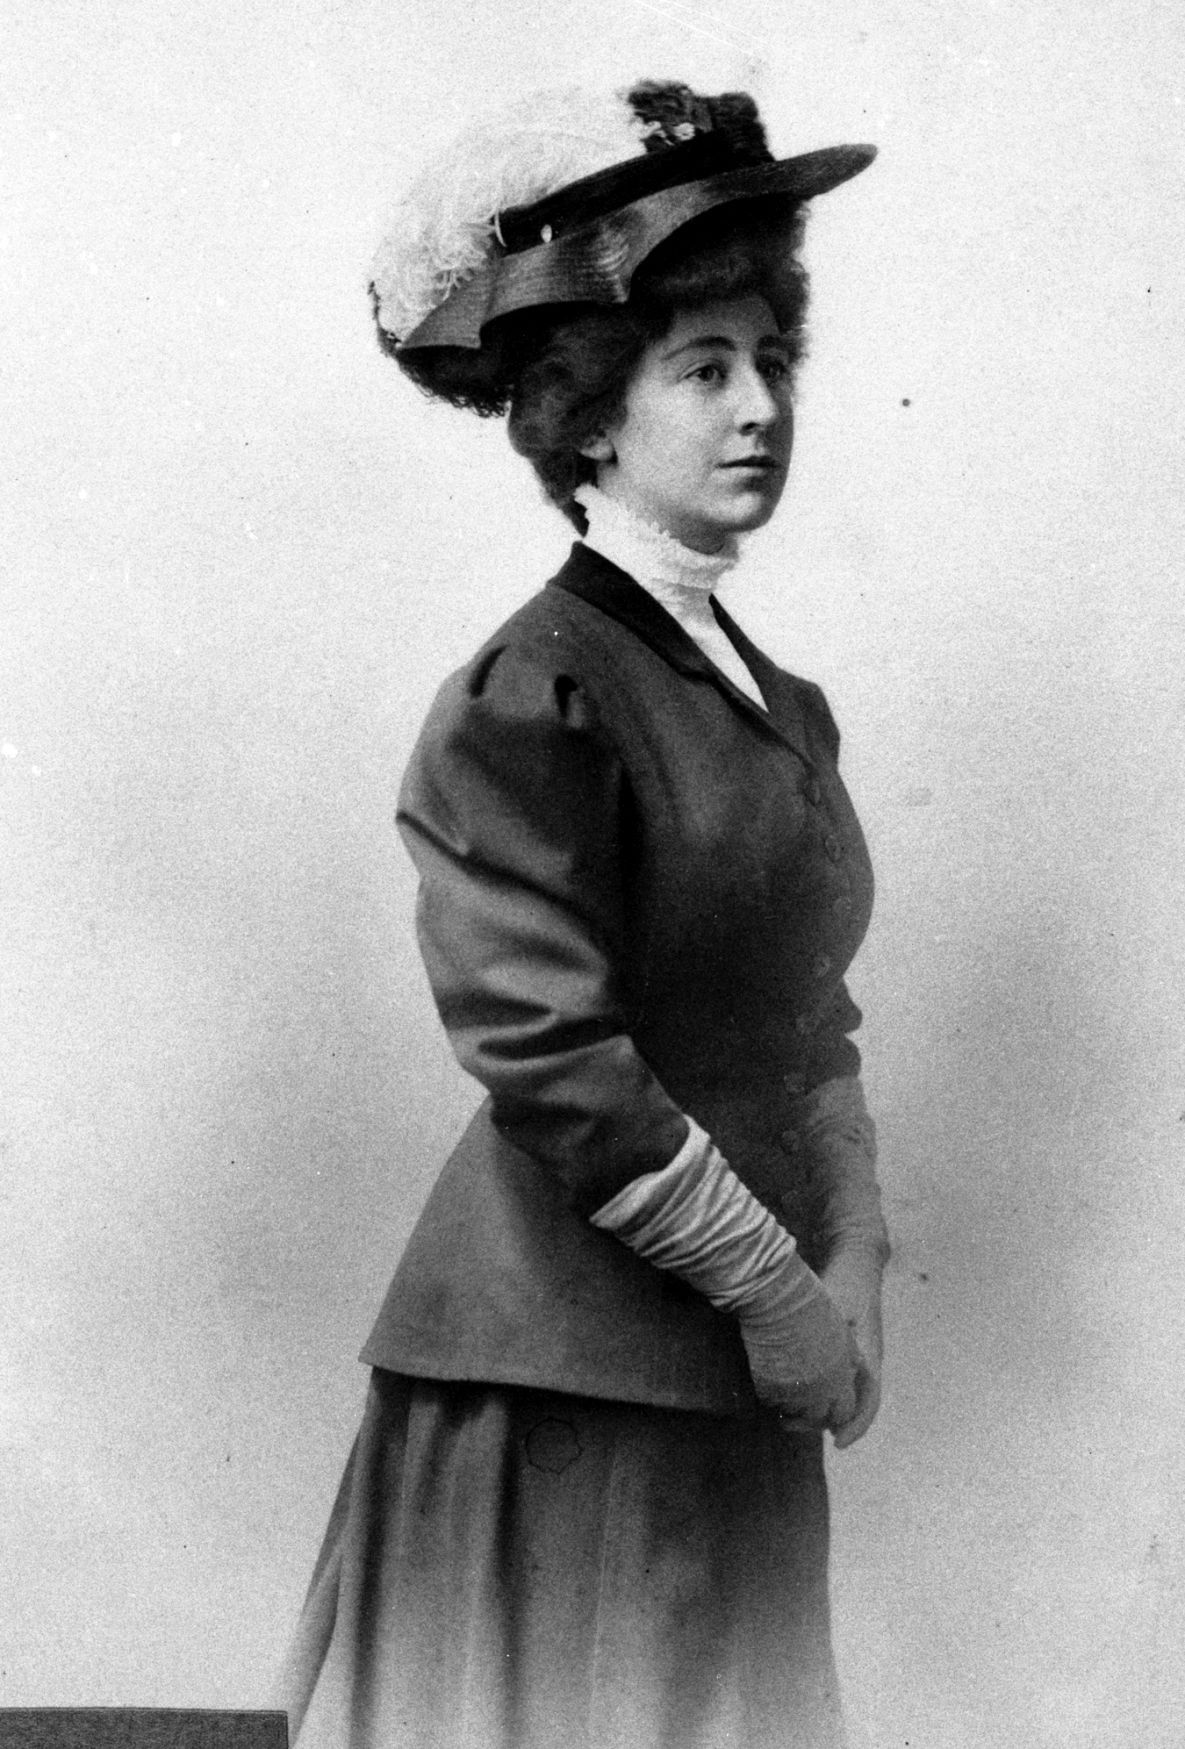
\includegraphics[max width=0.9\textwidth,max height=0.4\textheight]{{Images/rankin}.jpg}
    \end{center}
    \end{column}
    \end{columns}
}
\end{frame}
    

\begin{frame}[t]{Round 3, Answer 7}
\vspace{0.5em}
\begin{block}{Question}
Who wrote \emph{Little Women}\,?
\end{block}
\visible<2->{
    \begin{columns}[T,totalwidth=\linewidth]
    \begin{column}{0.35\linewidth}
    \begin{block}{Answer}
    Louisa May Alcott
    \end{block}
    \end{column}
    \begin{column}{0.6\linewidth}
    \begin{center}
    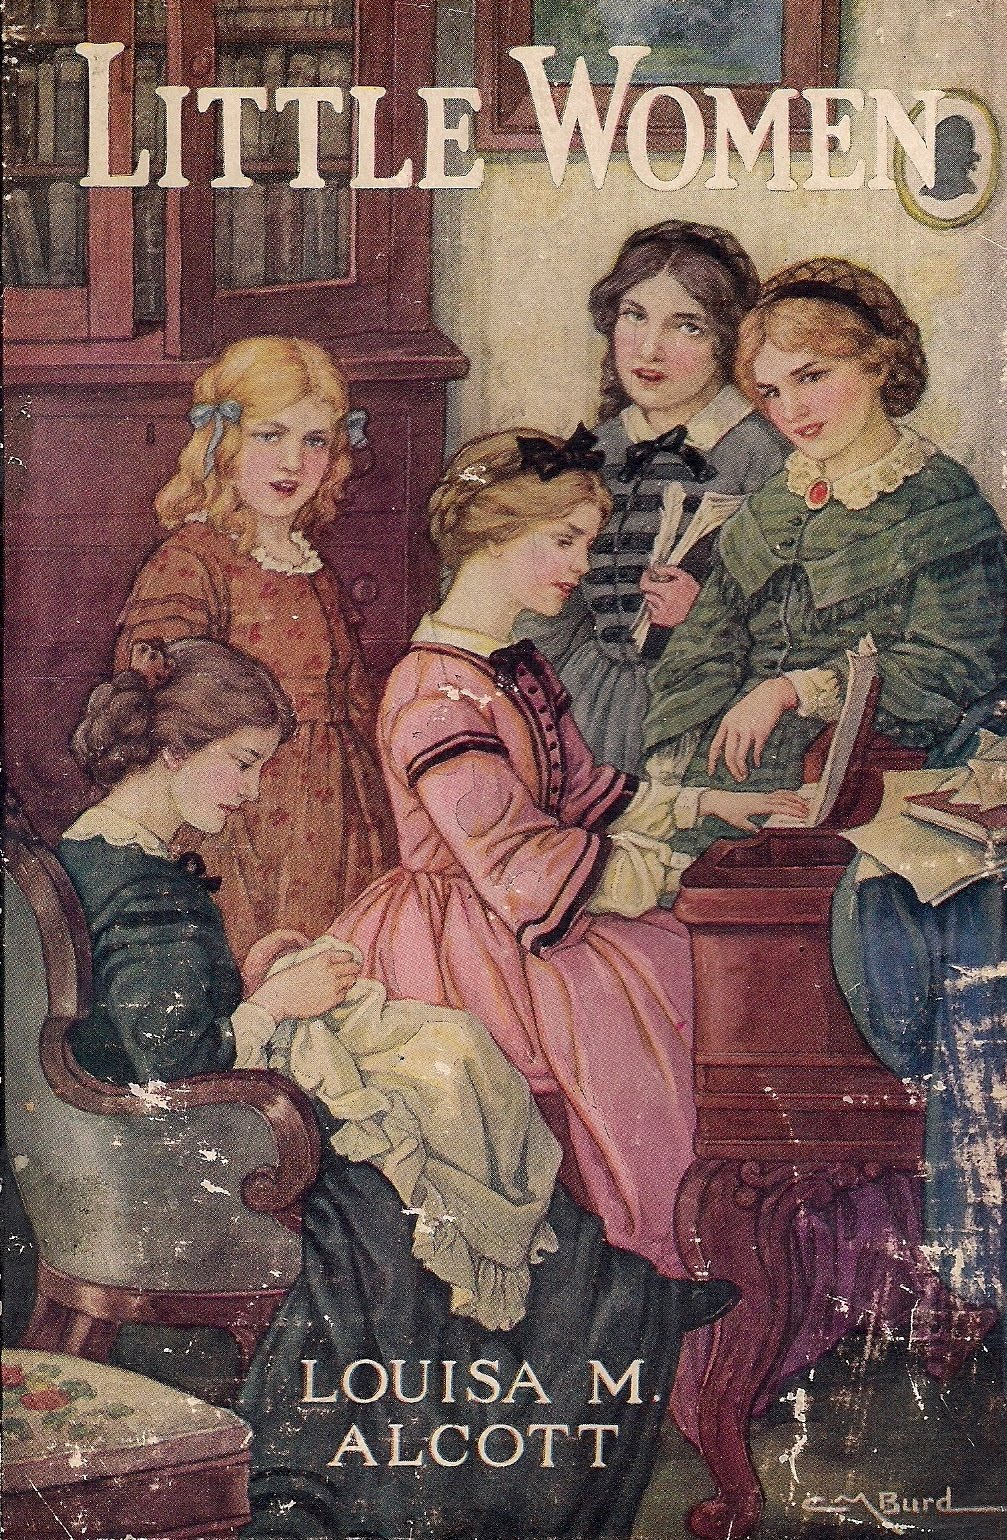
\includegraphics[max width=0.9\textwidth,max height=0.4\textheight]{{Images/little}.jpg}
    \end{center}
    \end{column}
    \end{columns}
}
\end{frame}
    

\begin{frame}[t]{Round 3, Answer 8}
\vspace{0.5em}
\begin{block}{Question}
Who designed the Vietnam War Memorial on the Mall in Washington, D.C.?
\end{block}
\visible<2->{
    \begin{columns}[T,totalwidth=\linewidth]
    \begin{column}{0.35\linewidth}
    \begin{block}{Answer}
    Maya Lin
    \end{block}
    \end{column}
    \begin{column}{0.6\linewidth}
    \begin{center}
    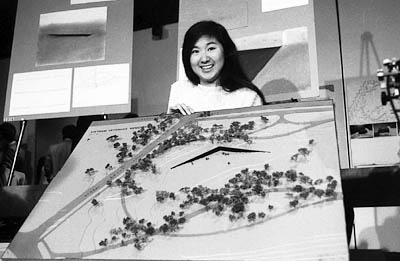
\includegraphics[max width=0.9\textwidth,max height=0.4\textheight]{{Images/mayalin}.jpg}
    \end{center}
    \end{column}
    \end{columns}
}
\end{frame}
    

\begin{frame}[t]{Round 3, Answer 9}
\vspace{0.5em}
\begin{block}{Question}
Which woman wrote a book about the absence of birdsong that brought attention to the environmental movement?
\end{block}
\visible<2->{
    \begin{columns}[T,totalwidth=\linewidth]
    \begin{column}{0.35\linewidth}
    \begin{block}{Answer}
    Rachel Carson
    \end{block}
    \end{column}
    \begin{column}{0.6\linewidth}
    \begin{center}
    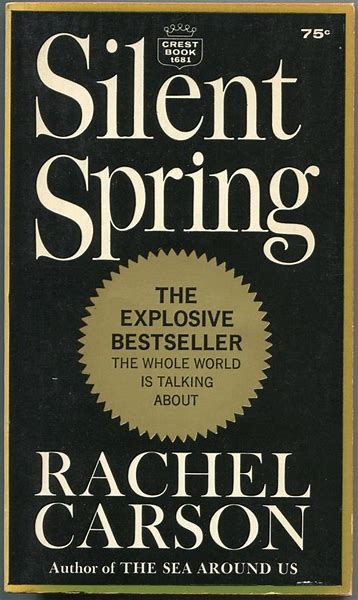
\includegraphics[max width=0.9\textwidth,max height=0.4\textheight]{{Images/silentspring}.jpeg}
    \end{center}
    \end{column}
    \end{columns}
}
\end{frame}
    

\begin{frame}[t]{Round 3, Answer 10}
\vspace{0.5em}
\begin{block}{Question}
Clara Barton founded and served as the first president of what organization?
\end{block}
\visible<2->{
    \begin{columns}[T,totalwidth=\linewidth]
    \begin{column}{0.35\linewidth}
    \begin{block}{Answer}
    The Red Cross
    \end{block}
    \end{column}
    \begin{column}{0.6\linewidth}
    \begin{center}
    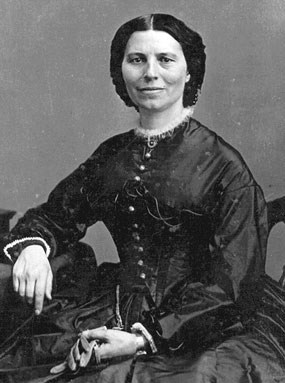
\includegraphics[max width=0.9\textwidth,max height=0.4\textheight]{{Images/barton}.jpg}
    \end{center}
    \end{column}
    \end{columns}
}
\end{frame}
    

\def\thisSectionName{Science}
\section{Round 4}
    

\subsection*{Q1}
\begin{frame}[t]{Round 4, Question 1}
\vspace{0.5em}
\begin{block}{Question}
At what temperature are Fahrenheit and Celsius represented by the same number?
\end{block}
\end{frame}
    

\subsection*{Q2}
\begin{frame}[t]{Round 4, Question 2}
\vspace{0.5em}
\begin{block}{Question}
Which two elements on the periodic table are liquid at room temperature and standard pressure?
\end{block}
\end{frame}
    

\subsection*{Q3}
\begin{frame}[t]{Round 4, Question 3}
\vspace{0.5em}
\begin{block}{Question}
Which biologist is considered the father of the rules of heredity/inheritance?
\end{block}
\end{frame}
    

\subsection*{Q4}
\begin{frame}[t]{Round 4, Question 4}
\vspace{0.5em}
\begin{block}{Question}
What physicist came up with the three laws of motion?
\end{block}
\end{frame}
    

\subsection*{Q5}
\begin{frame}[t]{Round 4, Question 5}
\vspace{0.5em}
\begin{block}{Question}
Who is the only person to have won the Nobel prize in two different scientific fields?
\end{block}
\end{frame}
    

\subsection*{Q6}
\begin{frame}[t]{Round 4, Question 6}
\vspace{0.5em}
\begin{block}{Question}
What is the chemical formula for table salt?
\end{block}
\end{frame}
    

\subsection*{Q7}
\begin{frame}[t]{Round 4, Question 7}
\vspace{0.5em}
\begin{block}{Question}
What is the most abundant gas in Earth's atmosphere?
\end{block}
\end{frame}
    

\subsection*{Q8}
\begin{frame}[t]{Round 4, Question 8}
\vspace{0.5em}
\begin{block}{Question}
Name either of the two-word phrases that describe a color change caused by an object's movement away from you.
\end{block}
\end{frame}
    

\subsection*{Q9}
\begin{frame}[t]{Round 4, Question 9}
\vspace{0.5em}
\begin{block}{Question}
Which is the heaviest internal organ in the human body?
\end{block}
\end{frame}
    

\subsection*{Q10}
\begin{frame}[t]{Round 4, Question 10}
\vspace{0.5em}
\begin{block}{Question}
In the equation \(E=mc^2\), what does \(c\) represent?
\end{block}
\end{frame}
    
\subsection{Answers}

\begin{frame}[t]{Round 4, Answer 1}
\vspace{0.5em}
\begin{block}{Question}
At what temperature are Fahrenheit and Celsius represented by the same number?
\end{block}
\visible<2->{
    \begin{columns}[T,totalwidth=\linewidth]
    \begin{column}{0.35\linewidth}
    \begin{block}{Answer}
    -40
    \end{block}
    \end{column}
    \begin{column}{0.6\linewidth}
    \begin{center}
    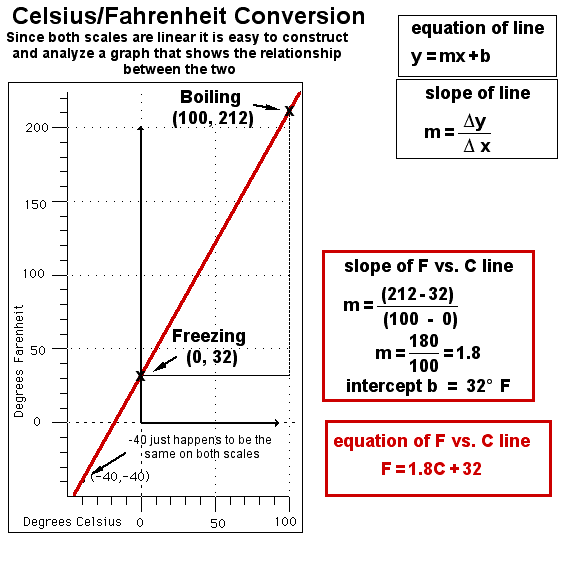
\includegraphics[max width=0.9\textwidth,max height=0.4\textheight]{{Images/degrees}.png}
    \end{center}
    \end{column}
    \end{columns}
}
\end{frame}
    

\begin{frame}[t]{Round 4, Answer 2}
\vspace{0.5em}
\begin{block}{Question}
Which two elements on the periodic table are liquid at room temperature and standard pressure?
\end{block}
\visible<2->{
    \begin{columns}[T,totalwidth=\linewidth]
    \begin{column}{0.35\linewidth}
    \begin{block}{Answer}
    Bromine (Br) and mercury (Hg)
    \end{block}
    \end{column}
    \begin{column}{0.6\linewidth}
    \begin{center}
    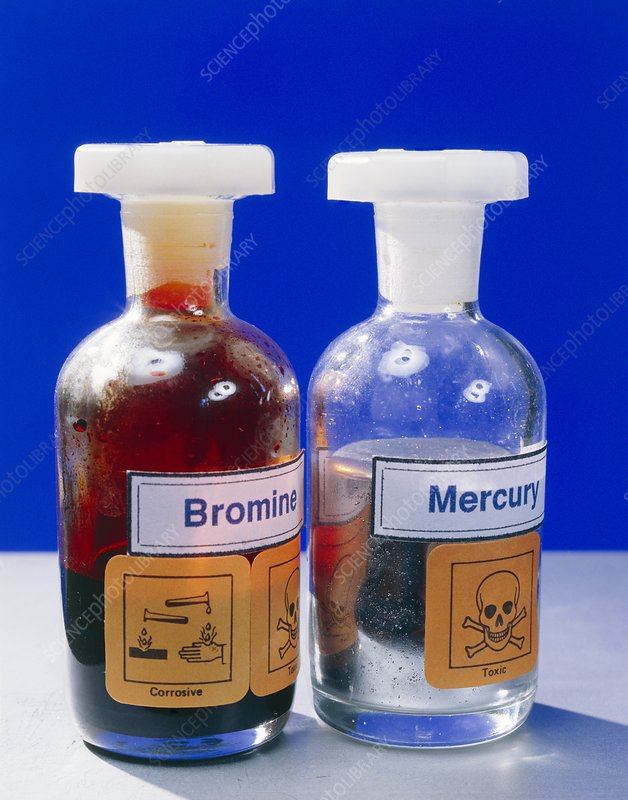
\includegraphics[max width=0.9\textwidth,max height=0.4\textheight]{{Images/bromine}.jpg}
    \end{center}
    \end{column}
    \end{columns}
}
\end{frame}
    

\begin{frame}[t]{Round 4, Answer 3}
\vspace{0.5em}
\begin{block}{Question}
Which biologist is considered the father of the rules of heredity/inheritance?
\end{block}
\visible<2->{
    \begin{columns}[T,totalwidth=\linewidth]
    \begin{column}{0.35\linewidth}
    \begin{block}{Answer}
    Gregor Mendel
    \end{block}
    \end{column}
    \begin{column}{0.6\linewidth}
    \begin{center}
    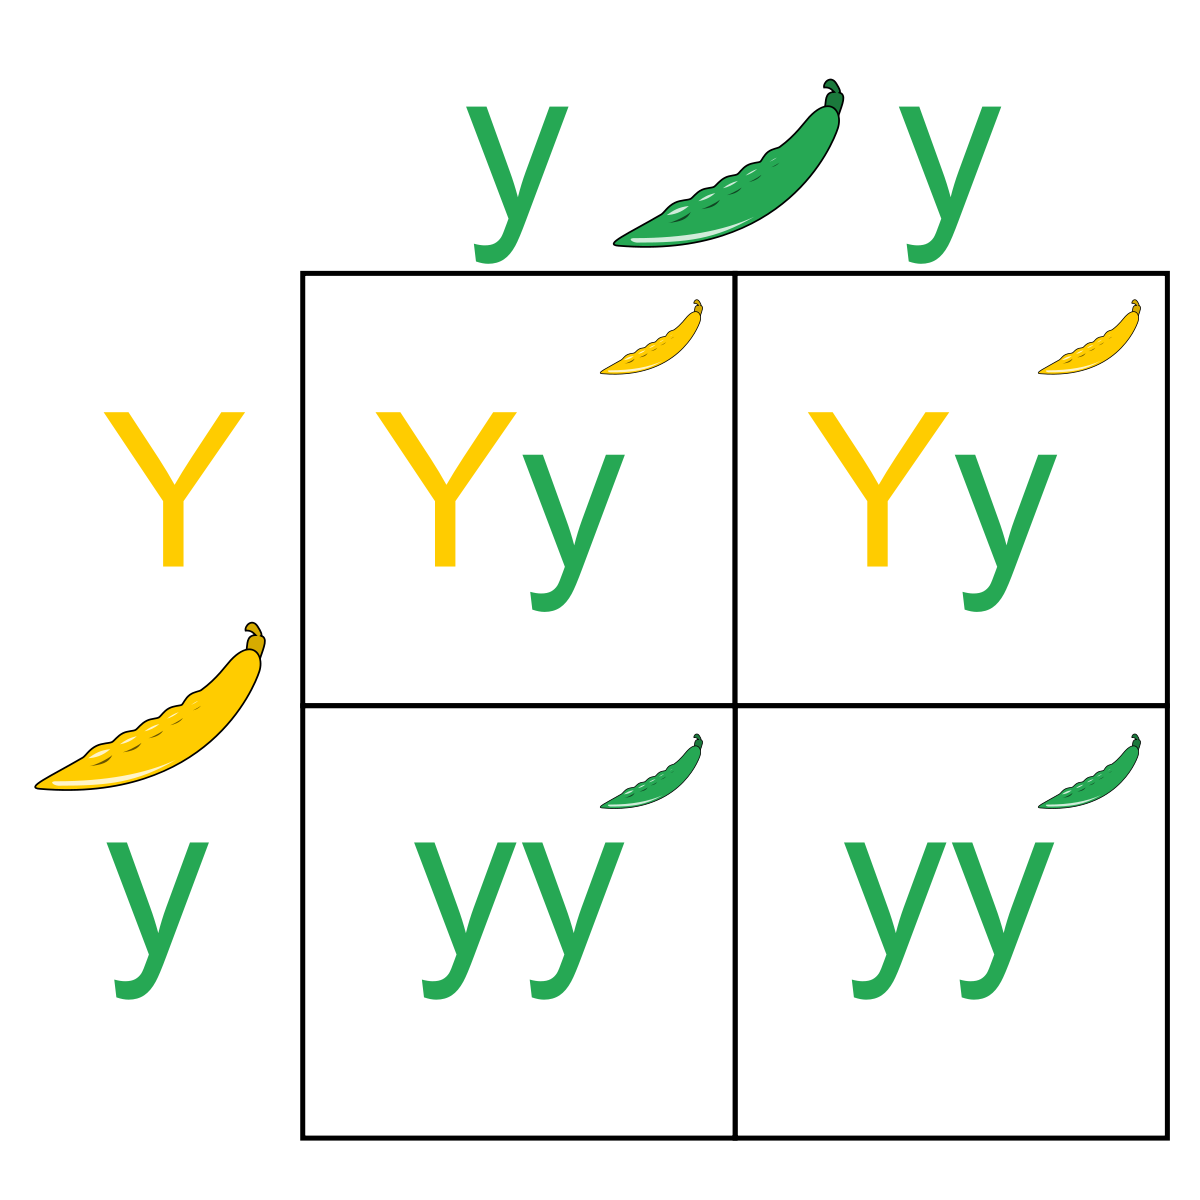
\includegraphics[max width=0.9\textwidth,max height=0.4\textheight]{{Images/punnett}.png}
    \end{center}
    \end{column}
    \end{columns}
}
\end{frame}
    

\begin{frame}[t]{Round 4, Answer 4}
\vspace{0.5em}
\begin{block}{Question}
What physicist came up with the three laws of motion?
\end{block}
\visible<2->{
    \begin{columns}[T,totalwidth=\linewidth]
    \begin{column}{0.35\linewidth}
    \begin{block}{Answer}
    Isaac Newton
    \end{block}
    \end{column}
    \begin{column}{0.6\linewidth}
    \begin{center}
    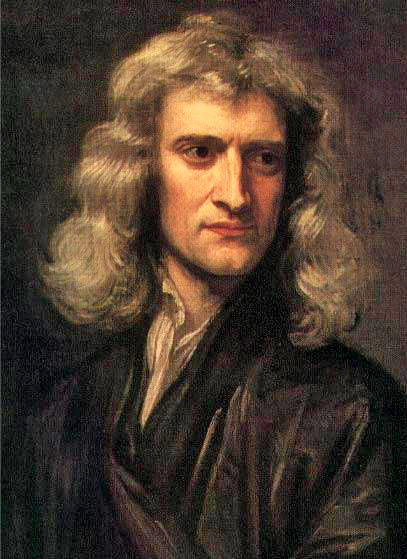
\includegraphics[max width=0.9\textwidth,max height=0.4\textheight]{{Images/newton}.jpg}
    \end{center}
    \end{column}
    \end{columns}
}
\end{frame}
    

\begin{frame}[t]{Round 4, Answer 5}
\vspace{0.5em}
\begin{block}{Question}
Who is the only person to have won the Nobel prize in two different scientific fields?
\end{block}
\visible<2->{
    \begin{columns}[T,totalwidth=\linewidth]
    \begin{column}{0.35\linewidth}
    \begin{block}{Answer}
    Marie Curie (Physics and Chemistry)
    \end{block}
    \end{column}
    \begin{column}{0.6\linewidth}
    \begin{center}
    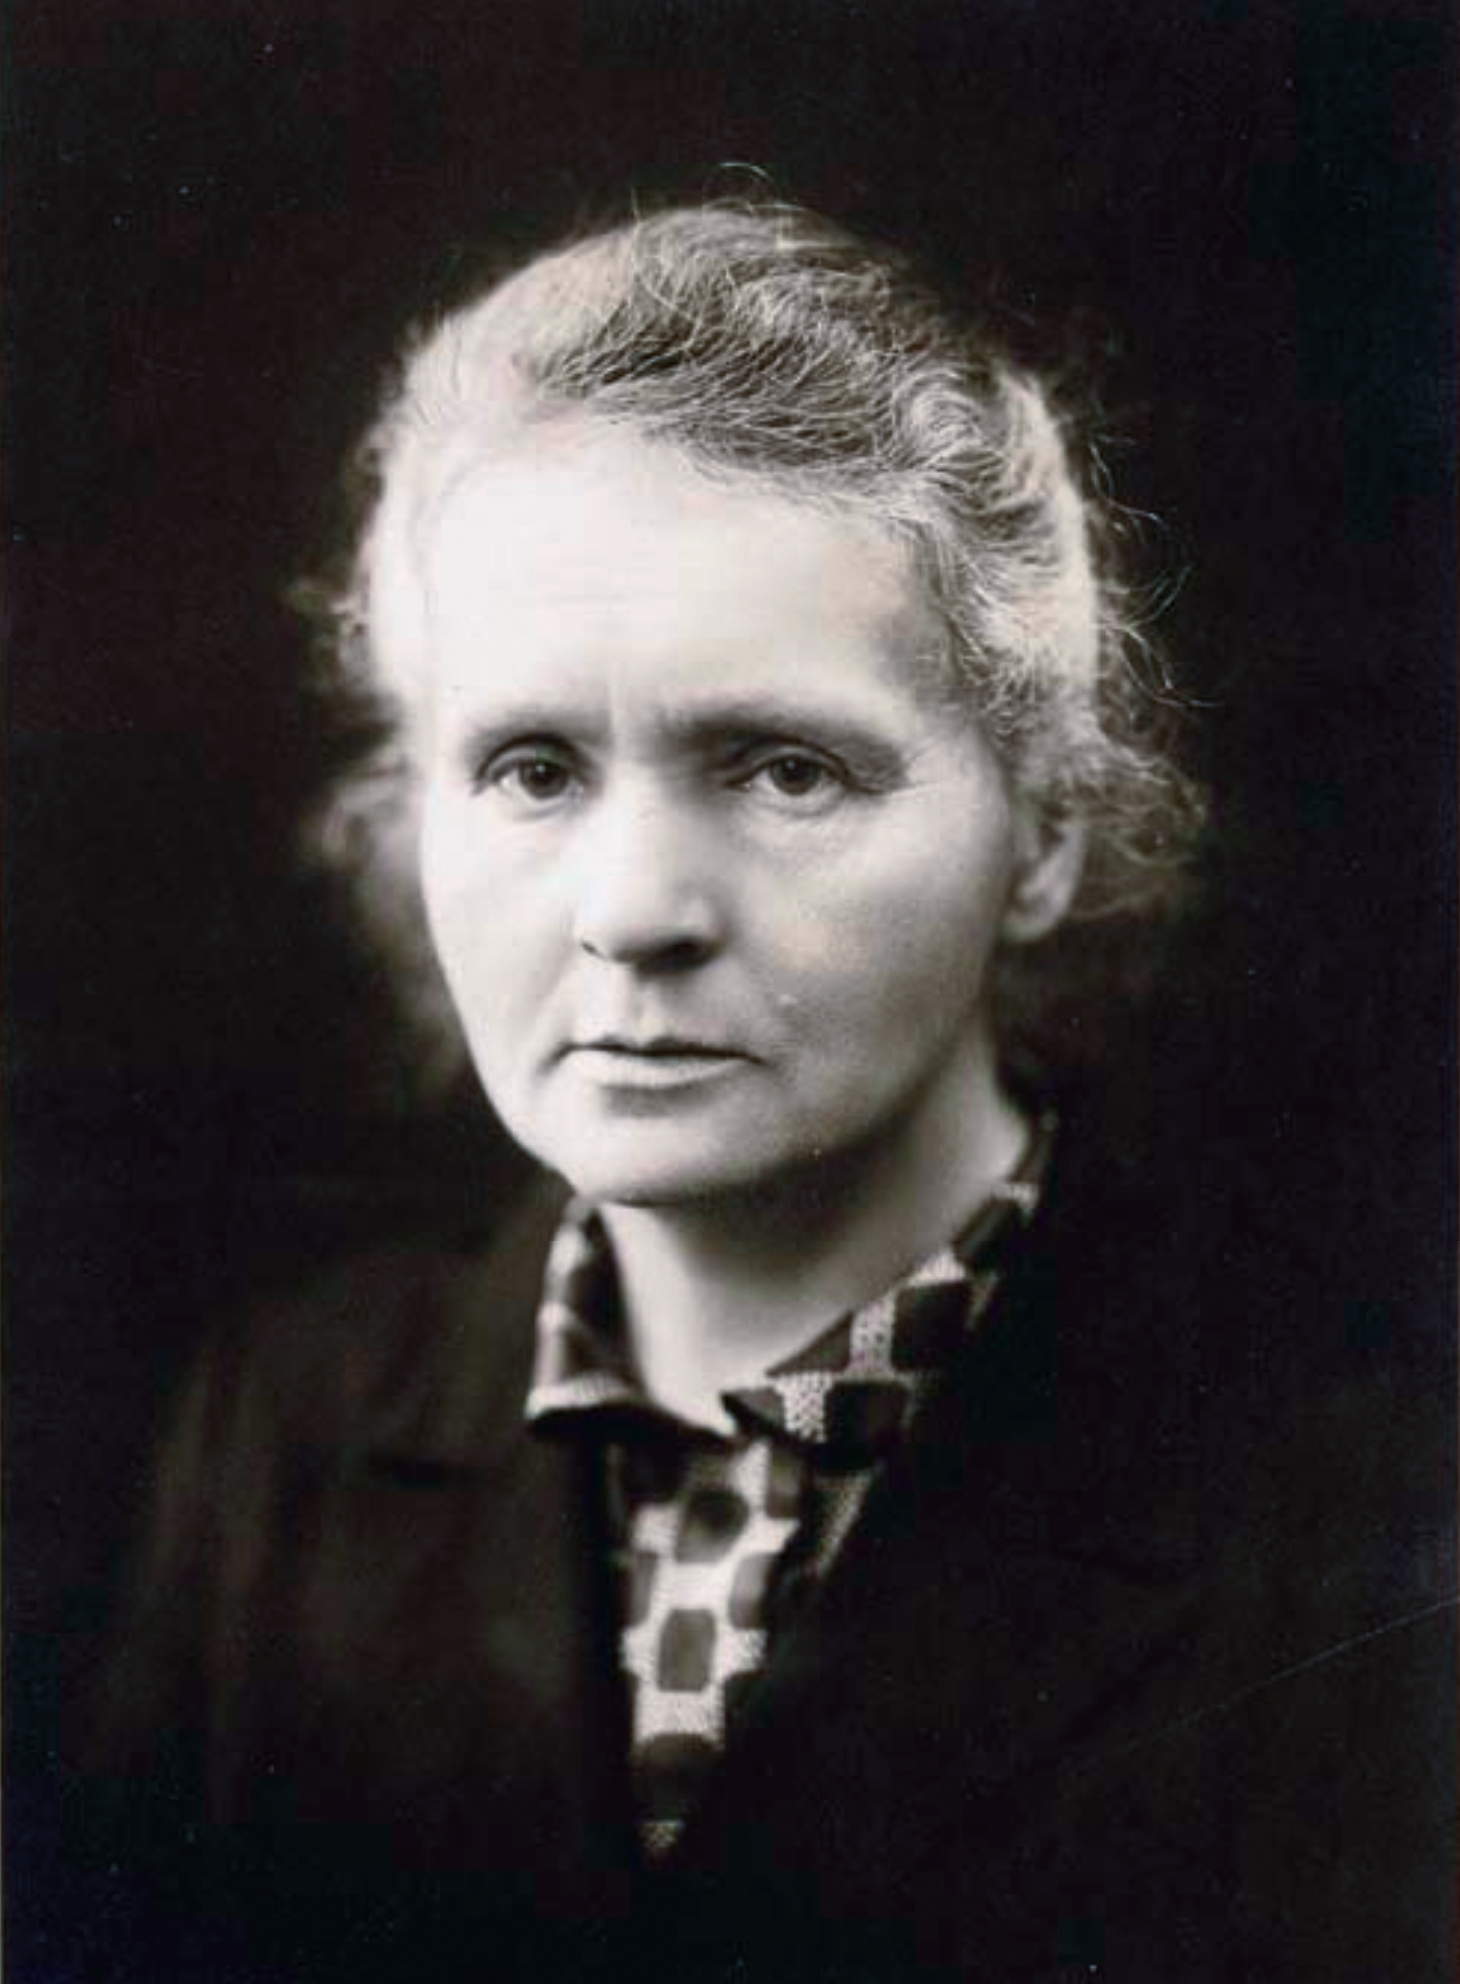
\includegraphics[max width=0.9\textwidth,max height=0.4\textheight]{{Images/curie}.jpg}
    \end{center}
    \end{column}
    \end{columns}
}
\end{frame}
    

\begin{frame}[t]{Round 4, Answer 6}
\vspace{0.5em}
\begin{block}{Question}
What is the chemical formula for table salt?
\end{block}
\visible<2->{
    \begin{columns}[T,totalwidth=\linewidth]
    \begin{column}{0.35\linewidth}
    \begin{block}{Answer}
    NaCl
    \end{block}
    \end{column}
    \begin{column}{0.6\linewidth}
    \begin{center}
    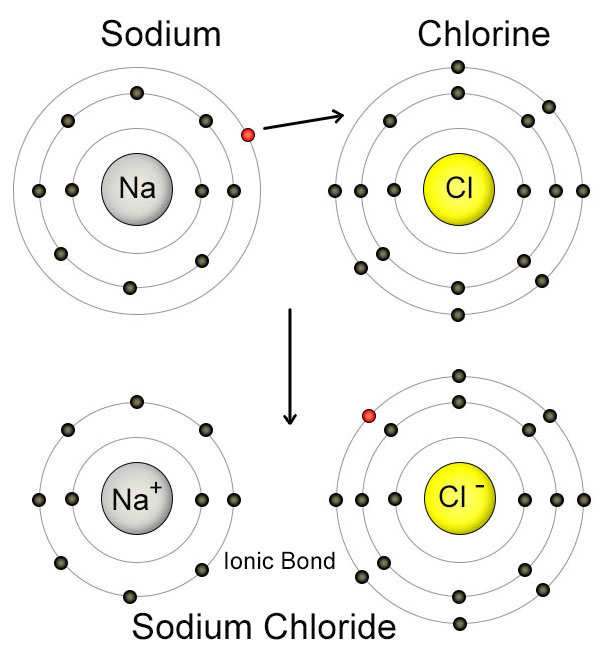
\includegraphics[max width=0.9\textwidth,max height=0.4\textheight]{{Images/nacl}.jpg}
    \end{center}
    \end{column}
    \end{columns}
}
\end{frame}
    

\begin{frame}[t]{Round 4, Answer 7}
\vspace{0.5em}
\begin{block}{Question}
What is the most abundant gas in Earth's atmosphere?
\end{block}
\visible<2->{
    \begin{columns}[T,totalwidth=\linewidth]
    \begin{column}{0.35\linewidth}
    \begin{block}{Answer}
    Nitrogen (77\%)
    \end{block}
    \end{column}
    \begin{column}{0.6\linewidth}
    \begin{center}
    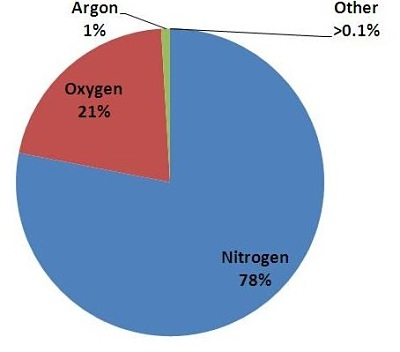
\includegraphics[max width=0.9\textwidth,max height=0.4\textheight]{{Images/atmosphere}.jpg}
    \end{center}
    \end{column}
    \end{columns}
}
\end{frame}
    

\begin{frame}[t]{Round 4, Answer 8}
\vspace{0.5em}
\begin{block}{Question}
Name either of the two-word phrases that describe a color change caused by an object's movement away from you.
\end{block}
\visible<2->{
    \begin{columns}[T,totalwidth=\linewidth]
    \begin{column}{0.35\linewidth}
    \begin{block}{Answer}
    Red shift or Doppler effect
    \end{block}
    \end{column}
    \begin{column}{0.6\linewidth}
    \begin{center}
    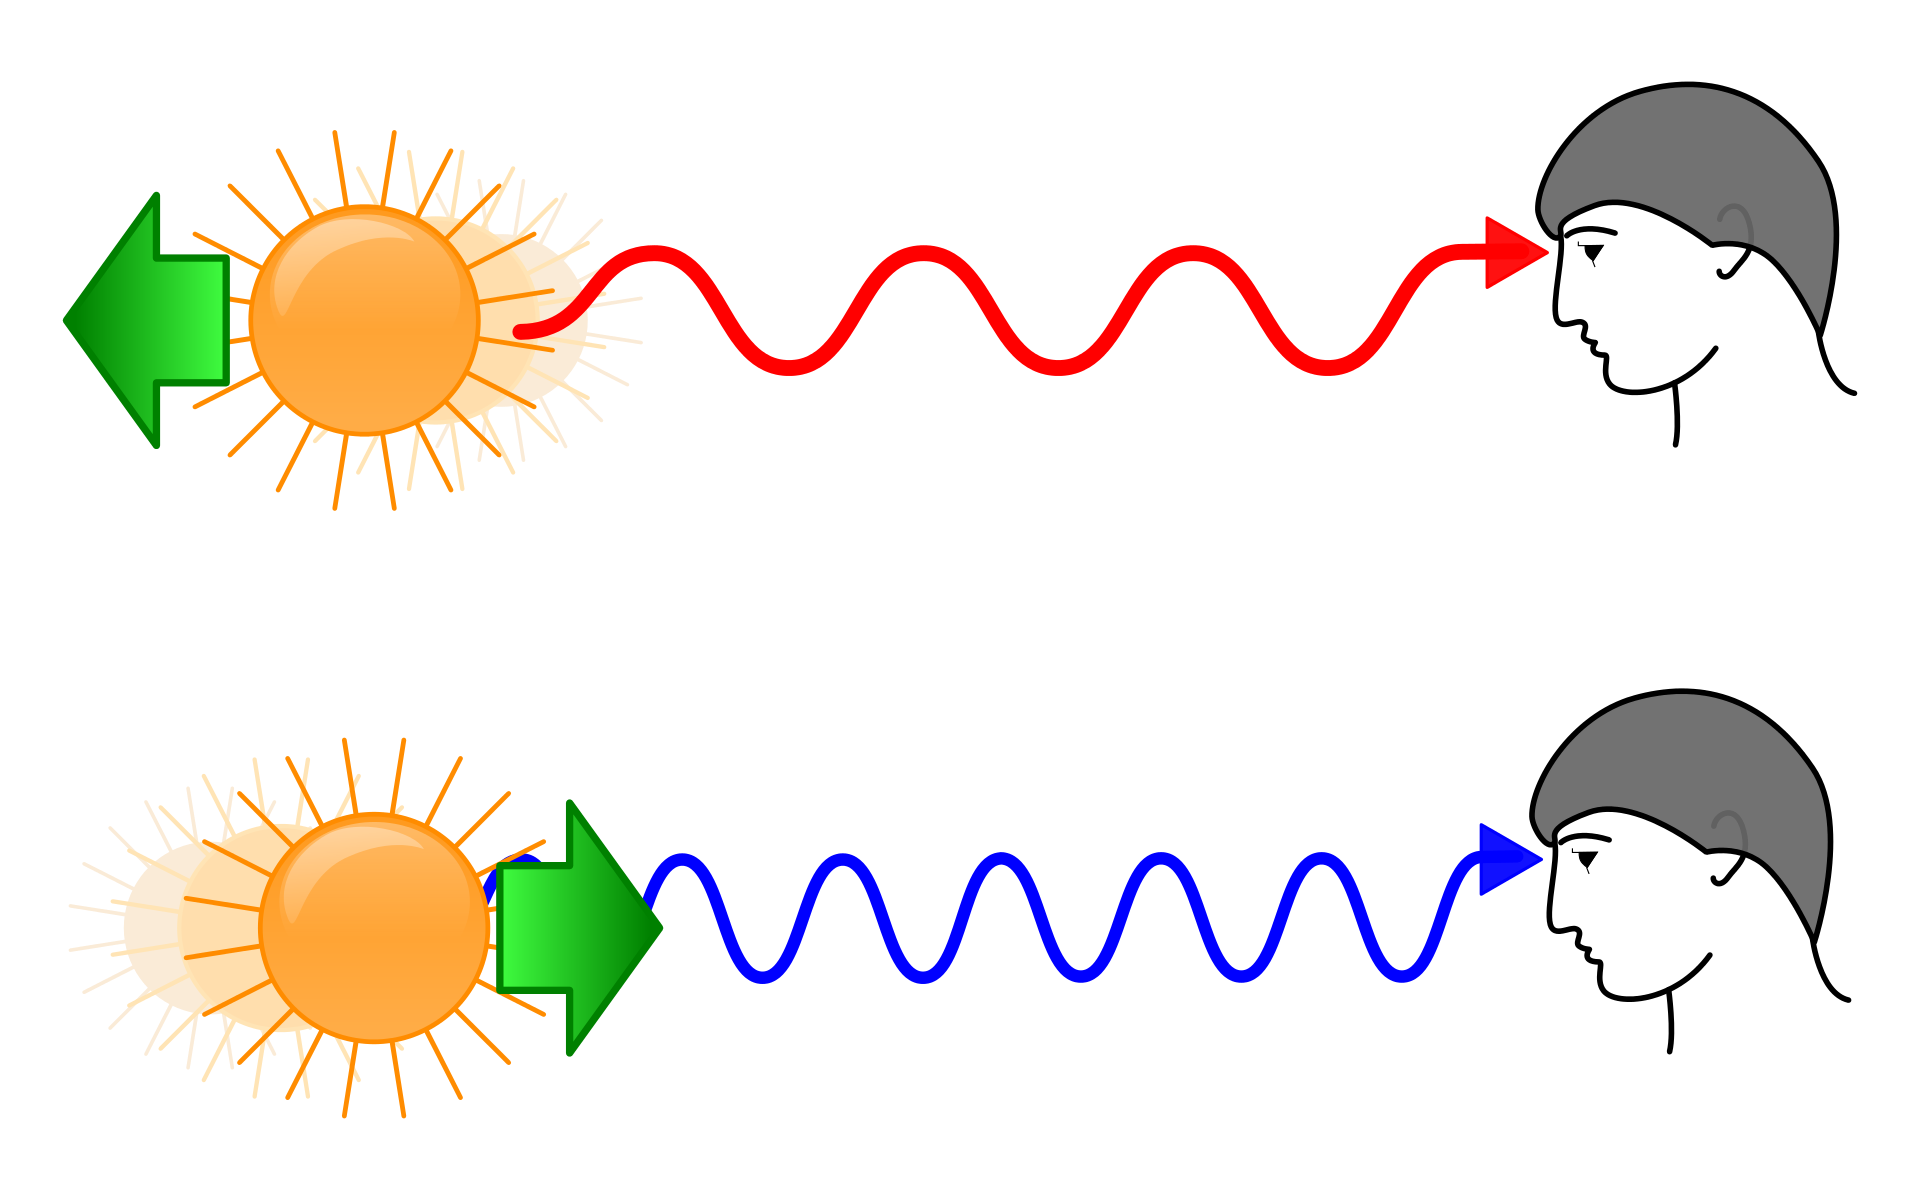
\includegraphics[max width=0.9\textwidth,max height=0.4\textheight]{{Images/redshift}.png}
    \end{center}
    \end{column}
    \end{columns}
}
\end{frame}
    

\begin{frame}[t]{Round 4, Answer 9}
\vspace{0.5em}
\begin{block}{Question}
Which is the heaviest internal organ in the human body?
\end{block}
\visible<2->{
    \begin{columns}[T,totalwidth=\linewidth]
    \begin{column}{0.35\linewidth}
    \begin{block}{Answer}
    The liver (approximately 3.5 lbs on average)
    \end{block}
    \end{column}
    \begin{column}{0.6\linewidth}
    \begin{center}
    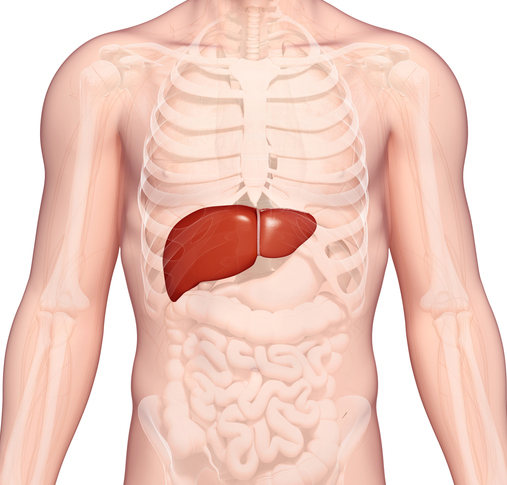
\includegraphics[max width=0.9\textwidth,max height=0.4\textheight]{{Images/liver-location}.jpg}
    \end{center}
    \end{column}
    \end{columns}
}
\end{frame}
    

\begin{frame}[t]{Round 4, Answer 10}
\vspace{0.5em}
\begin{block}{Question}
In the equation \(E=mc^2\), what does \(c\) represent?
\end{block}
\visible<2->{
    \begin{block}{Answer}
    The speed of light
    \end{block}
}
\end{frame}
    

\def\thisSectionName{Plants and Animals}
\section{Round 5}
    

\subsection*{Q1}
\begin{frame}[t]{Round 5, Question 1}
\vspace{0.5em}
\begin{block}{Question}
In addition to the platypus, what is the only other species of mammal that lays eggs?
\end{block}
\end{frame}
    

\subsection*{Q2}
\begin{frame}[t]{Round 5, Question 2}
\vspace{0.5em}
\begin{block}{Question}
Members of which primate family have the longest arms relative to the size of their bodies?
\end{block}
\end{frame}
    

\subsection*{Q3}
\begin{frame}[t]{Round 5, Question 3}
\vspace{0.5em}
\begin{columns}[T,totalwidth=\linewidth]
\begin{column}{0.25\linewidth}
\begin{block}{Question}
What species of tree is this leaf from?
\end{block}
\end{column}
\begin{column}{0.7\linewidth}
\begin{center}
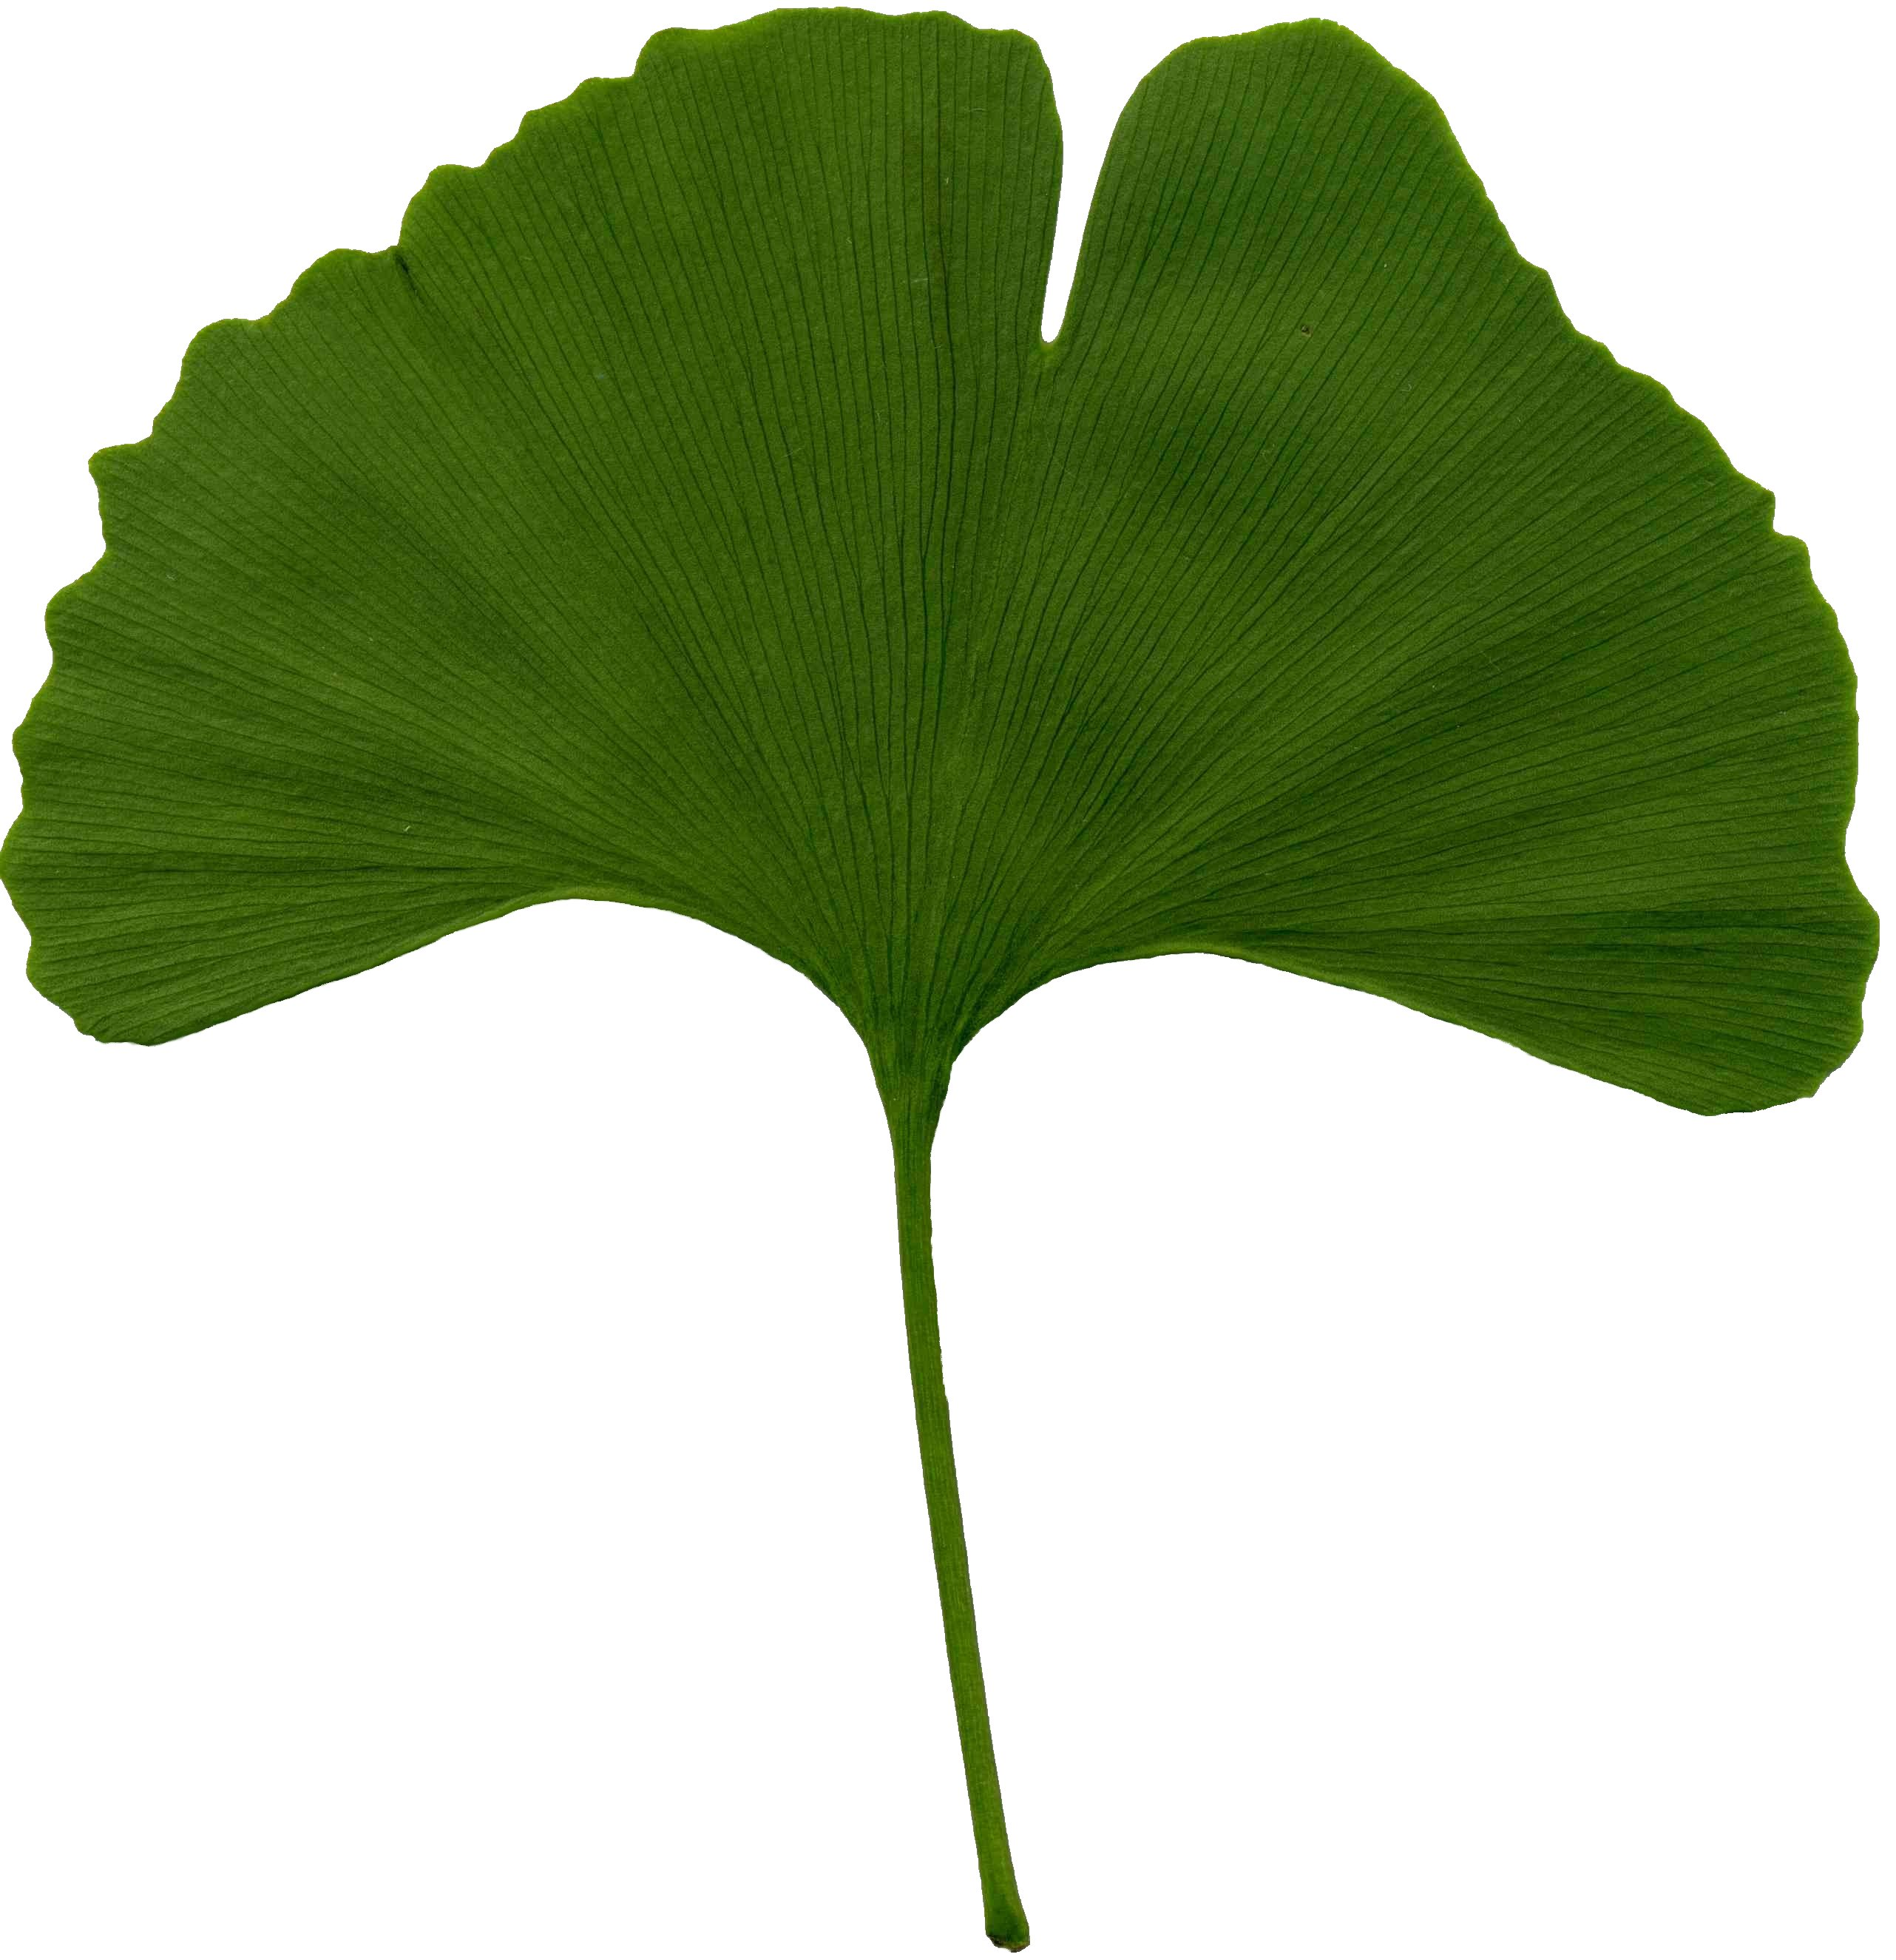
\includegraphics[max width=0.9\textwidth,max height=0.6\textheight]{{Images/gingko}.jpg}
\end{center}
\end{column}
\end{columns}
\end{frame}
    

\subsection*{Q4}
\begin{frame}[t]{Round 5, Question 4}
\vspace{0.5em}
\begin{block}{Question}
Name the three body sections that all insects' bodies are divided into.
\end{block}
\end{frame}
    

\subsection*{Q5}
\begin{frame}[t]{Round 5, Question 5}
\vspace{0.5em}
\begin{block}{Question}
A ``parliament'' is the collective noun for what animal?
\end{block}
\end{frame}
    

\subsection*{Q6}
\begin{frame}[t]{Round 5, Question 6}
\vspace{0.5em}
\begin{block}{Question}
What is the fastest animal species in the world? (Hint: it's not the cheetah.)
\end{block}
\end{frame}
    

\subsection*{Q7}
\begin{frame}[t]{Round 5, Question 7}
\vspace{0.5em}
\begin{block}{Question}
The tallest tree in the world belongs to what species?
\end{block}
\end{frame}
    

\subsection*{Q8}
\begin{frame}[t]{Round 5, Question 8}
\vspace{0.5em}
\begin{block}{Question}
What kind of animal produces gossamer?
\end{block}
\end{frame}
    

\subsection*{Q9}
\begin{frame}[t]{Round 5, Question 9}
\vspace{0.5em}
\begin{block}{Question}
How many hearts does an octopus have?
\end{block}
\end{frame}
    

\subsection*{Q10}
\begin{frame}[t]{Round 5, Question 10}
\vspace{0.5em}
\begin{block}{Question}
The bark of which tree species is used to produce aspirin?
\end{block}
\end{frame}
    
\subsection{Answers}

\begin{frame}[t]{Round 5, Answer 1}
\vspace{0.5em}
\begin{block}{Question}
In addition to the platypus, what is the only other species of mammal that lays eggs?
\end{block}
\visible<2->{
    \begin{columns}[T,totalwidth=\linewidth]
    \begin{column}{0.35\linewidth}
    \begin{block}{Answer}
    Echidna or spiny anteater
    \end{block}
    \end{column}
    \begin{column}{0.6\linewidth}
    \begin{center}
    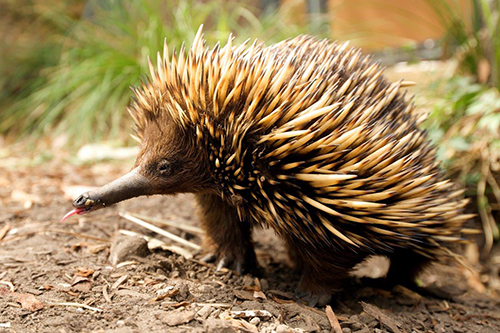
\includegraphics[max width=0.9\textwidth,max height=0.4\textheight]{{Images/echidna}.jpg}
    \end{center}
    \end{column}
    \end{columns}
}
\end{frame}
    

\begin{frame}[t]{Round 5, Answer 2}
\vspace{0.5em}
\begin{block}{Question}
Members of which primate family have the longest arms relative to the size of their bodies?
\end{block}
\visible<2->{
    \begin{columns}[T,totalwidth=\linewidth]
    \begin{column}{0.35\linewidth}
    \begin{block}{Answer}
    Gibbons
    \end{block}
    \end{column}
    \begin{column}{0.6\linewidth}
    \begin{center}
    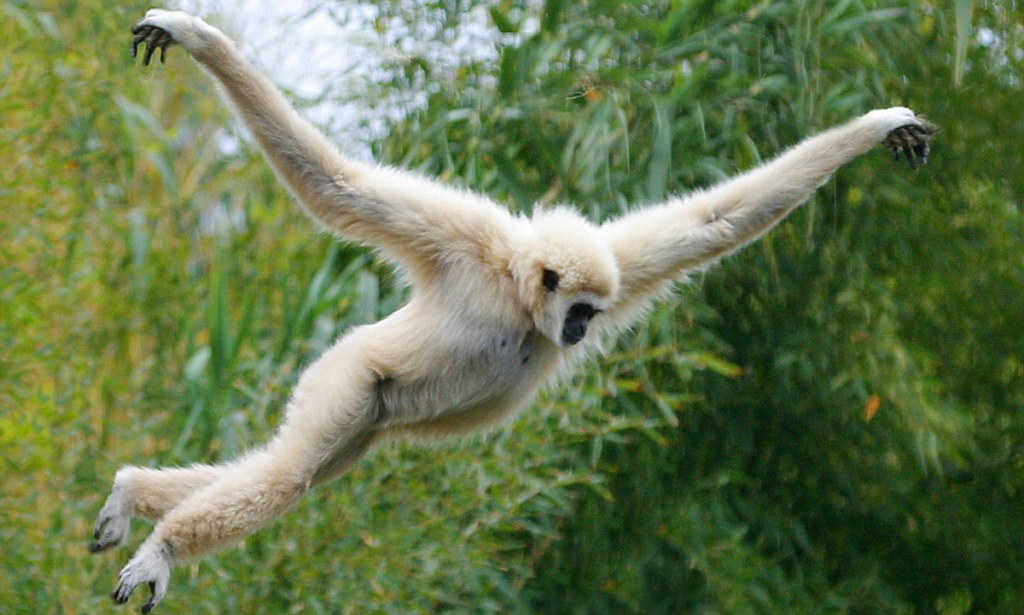
\includegraphics[max width=0.9\textwidth,max height=0.4\textheight]{{Images/gibbon}.jpg}
    \end{center}
    \end{column}
    \end{columns}
}
\end{frame}
    

\begin{frame}[t]{Round 5, Answer 3}
\vspace{0.5em}
\begin{columns}[T,totalwidth=\linewidth]
\begin{column}{0.35\linewidth}
\begin{block}{Question}
What species of tree is this leaf from?
\end{block}
\visible<2->{
    \begin{block}{Answer}
    Ginkgo (Biloba)
    \end{block}
}
\end{column}
\begin{column}{0.6\linewidth}
\begin{center}
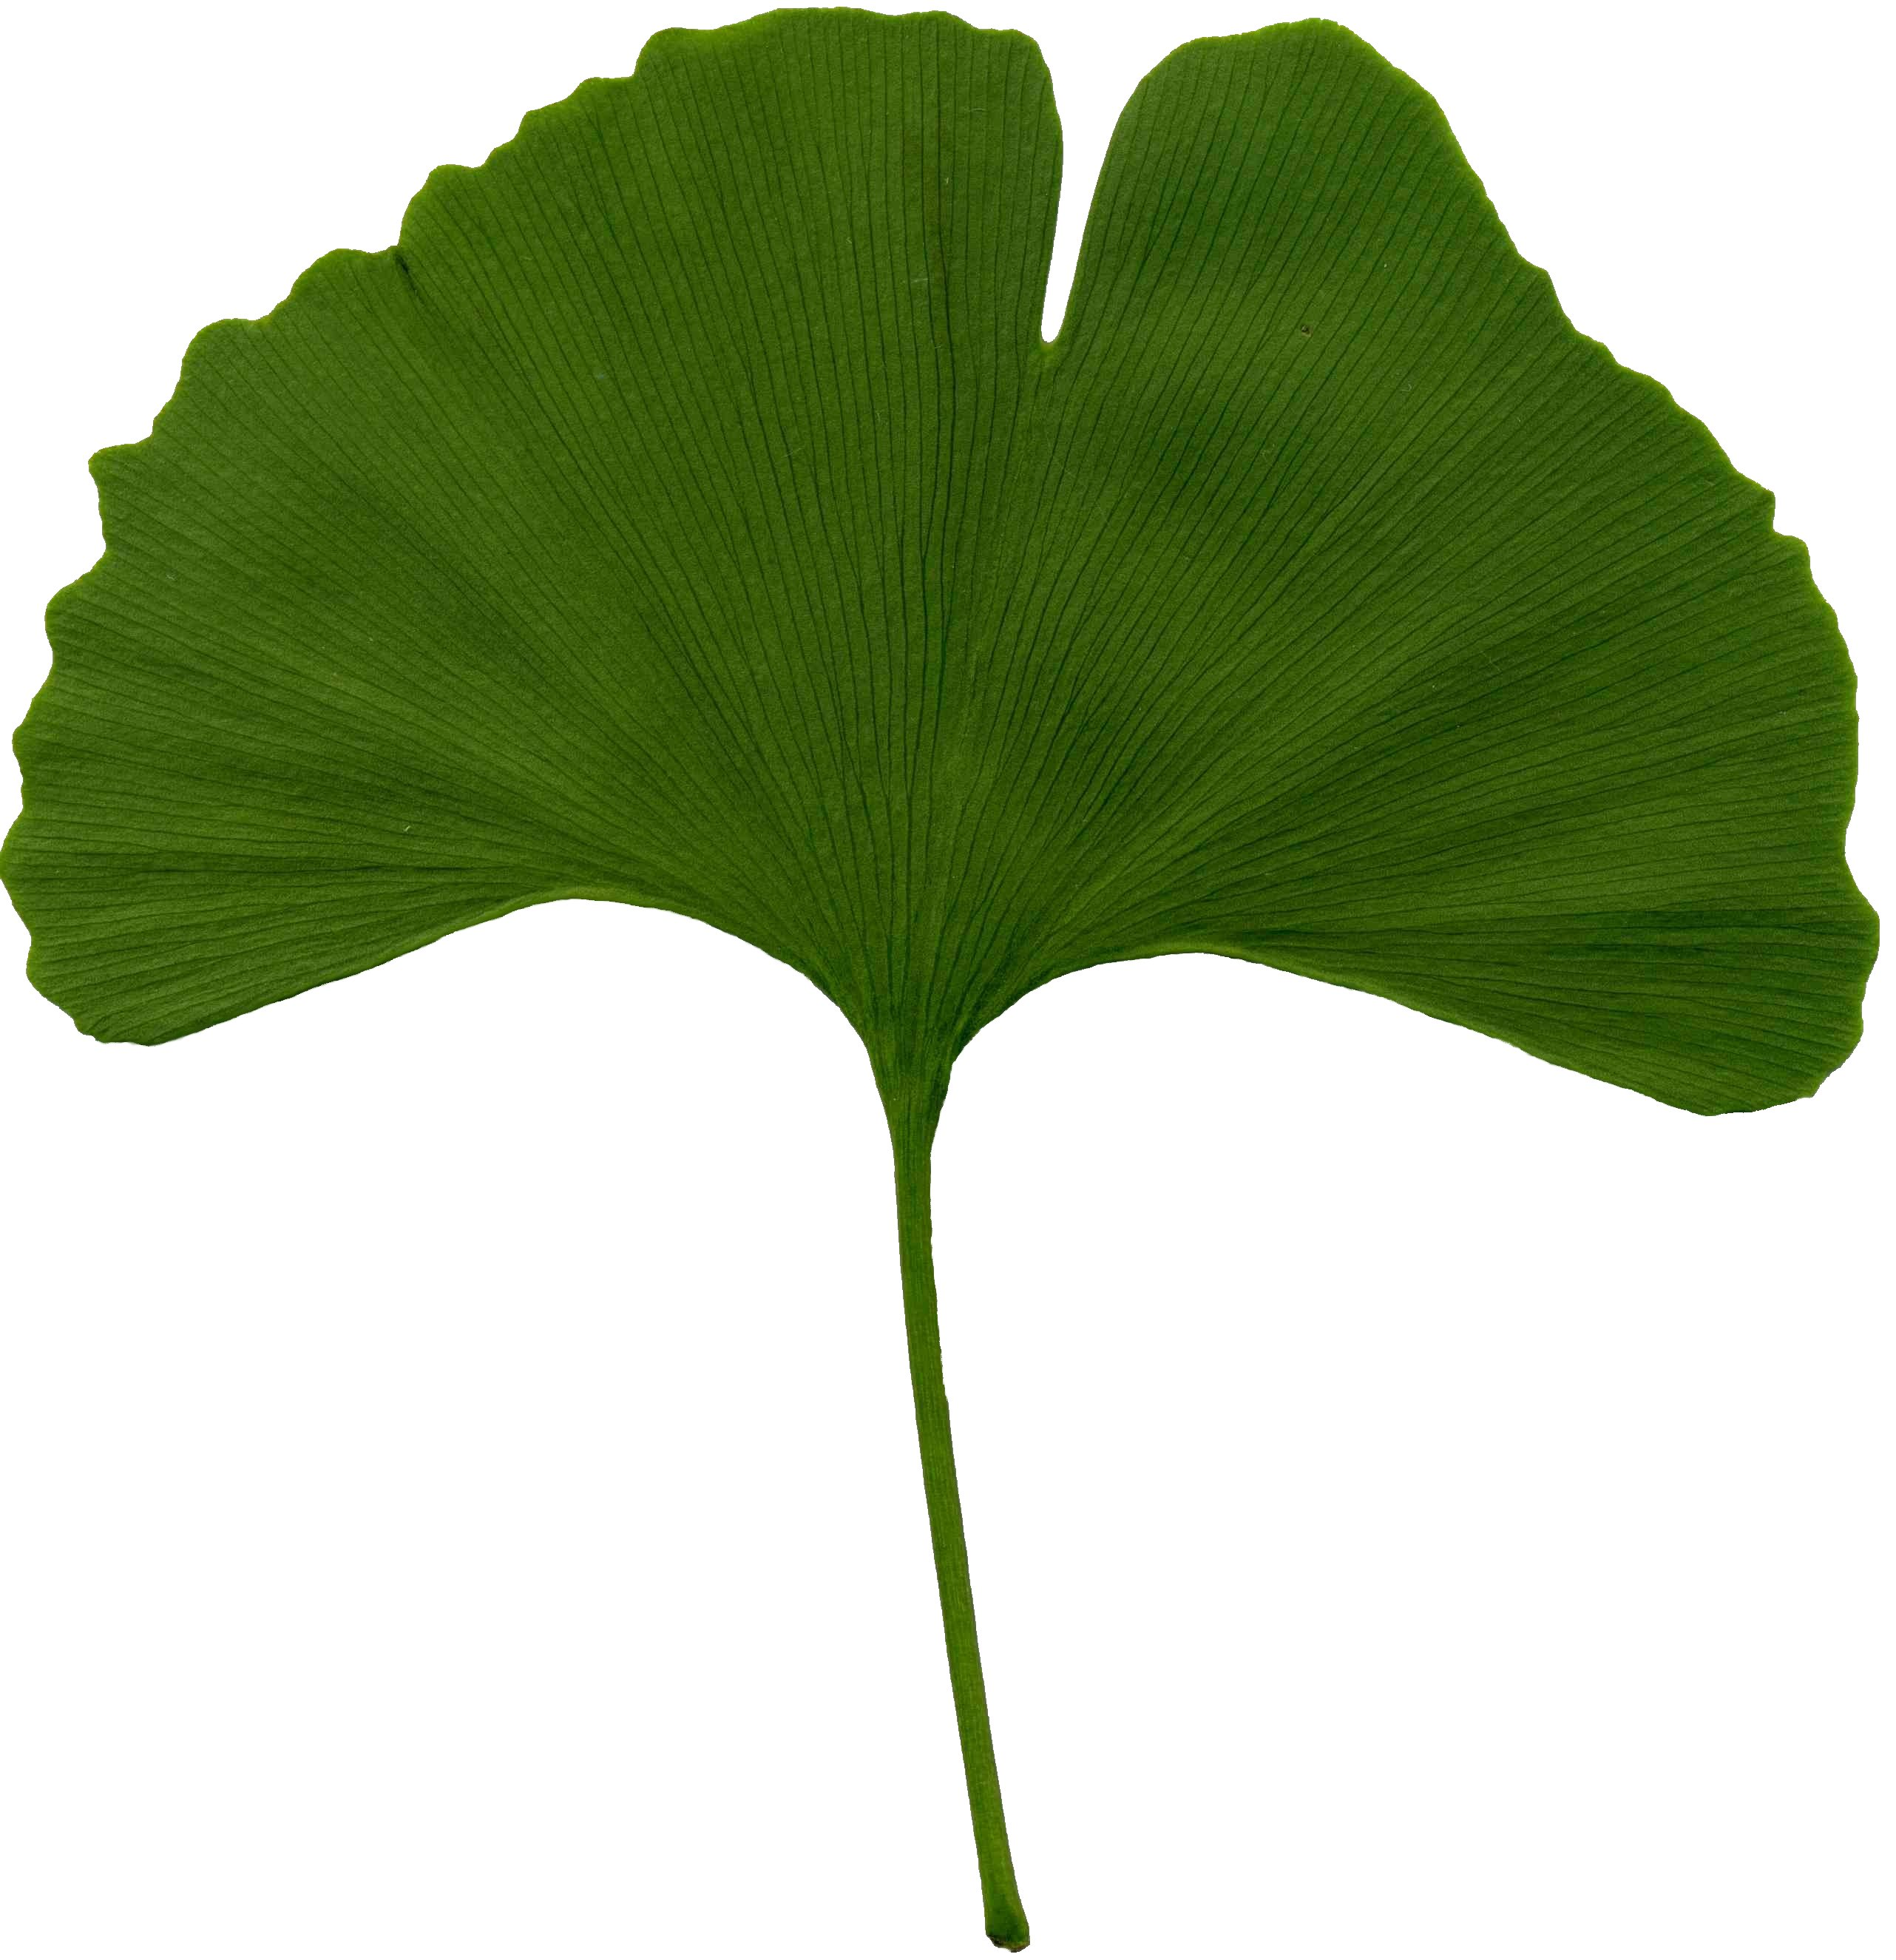
\includegraphics[max width=0.9\textwidth,max height=0.6\textheight]{{Images/gingko}.jpg}
\end{center}
\end{column}
\end{columns}
\end{frame}
    

\begin{frame}[t]{Round 5, Answer 4}
\vspace{0.5em}
\begin{block}{Question}
Name the three body sections that all insects' bodies are divided into.
\end{block}
\visible<2->{
    \begin{columns}[T,totalwidth=\linewidth]
    \begin{column}{0.35\linewidth}
    \begin{block}{Answer}
    Head, thorax, abdomen
    \end{block}
    \end{column}
    \begin{column}{0.6\linewidth}
    \begin{center}
    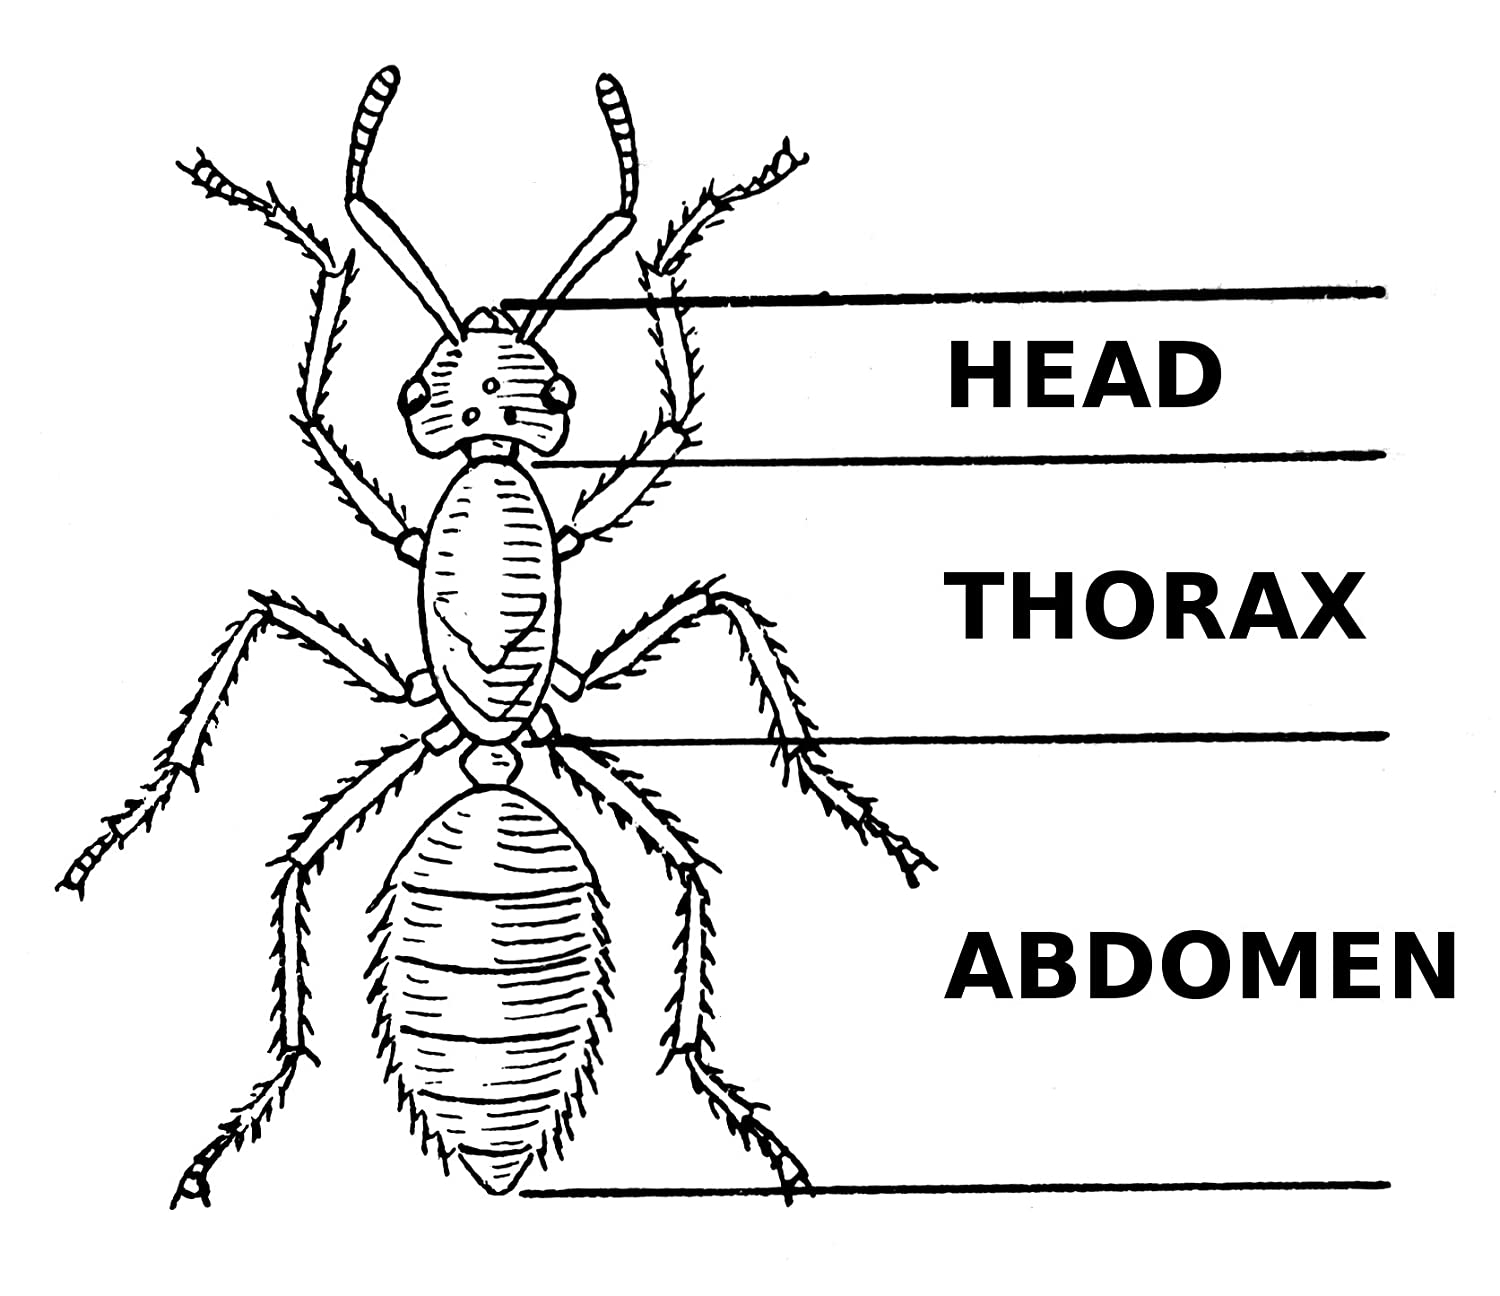
\includegraphics[max width=0.9\textwidth,max height=0.4\textheight]{{Images/insect}.jpg}
    \end{center}
    \end{column}
    \end{columns}
}
\end{frame}
    

\begin{frame}[t]{Round 5, Answer 5}
\vspace{0.5em}
\begin{block}{Question}
A ``parliament'' is the collective noun for what animal?
\end{block}
\visible<2->{
    \begin{columns}[T,totalwidth=\linewidth]
    \begin{column}{0.35\linewidth}
    \begin{block}{Answer}
    Owls
    \end{block}
    \end{column}
    \begin{column}{0.6\linewidth}
    \begin{center}
    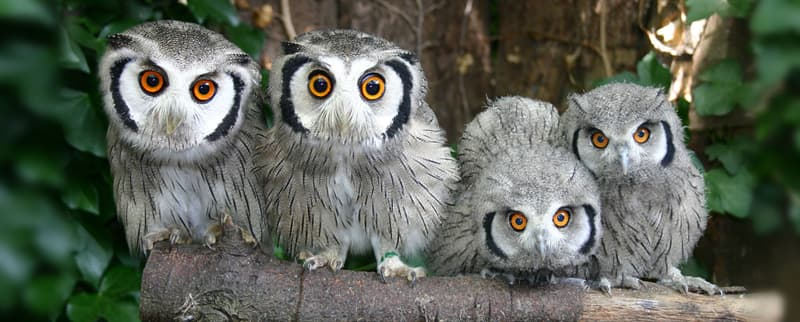
\includegraphics[max width=0.9\textwidth,max height=0.4\textheight]{{Images/owls}.jpg}
    \end{center}
    \end{column}
    \end{columns}
}
\end{frame}
    

\begin{frame}[t]{Round 5, Answer 6}
\vspace{0.5em}
\begin{block}{Question}
What is the fastest animal species in the world? (Hint: it's not the cheetah.)
\end{block}
\visible<2->{
    \begin{columns}[T,totalwidth=\linewidth]
    \begin{column}{0.35\linewidth}
    \begin{block}{Answer}
    Peregrine falcon (240 mph)
    \end{block}
    \end{column}
    \begin{column}{0.6\linewidth}
    \begin{center}
    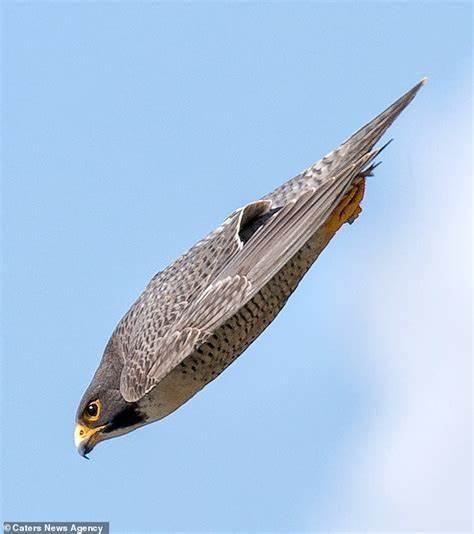
\includegraphics[max width=0.9\textwidth,max height=0.4\textheight]{{Images/peregrine}.jpeg}
    \end{center}
    \end{column}
    \end{columns}
}
\end{frame}
    

\begin{frame}[t]{Round 5, Answer 7}
\vspace{0.5em}
\begin{block}{Question}
The tallest tree in the world belongs to what species?
\end{block}
\visible<2->{
    \begin{columns}[T,totalwidth=\linewidth]
    \begin{column}{0.35\linewidth}
    \begin{block}{Answer}
    Redwood (\emph{Sequoia sempervirens}). The specific tree's name is Hyperion.
    \end{block}
    \end{column}
    \begin{column}{0.6\linewidth}
    \begin{center}
    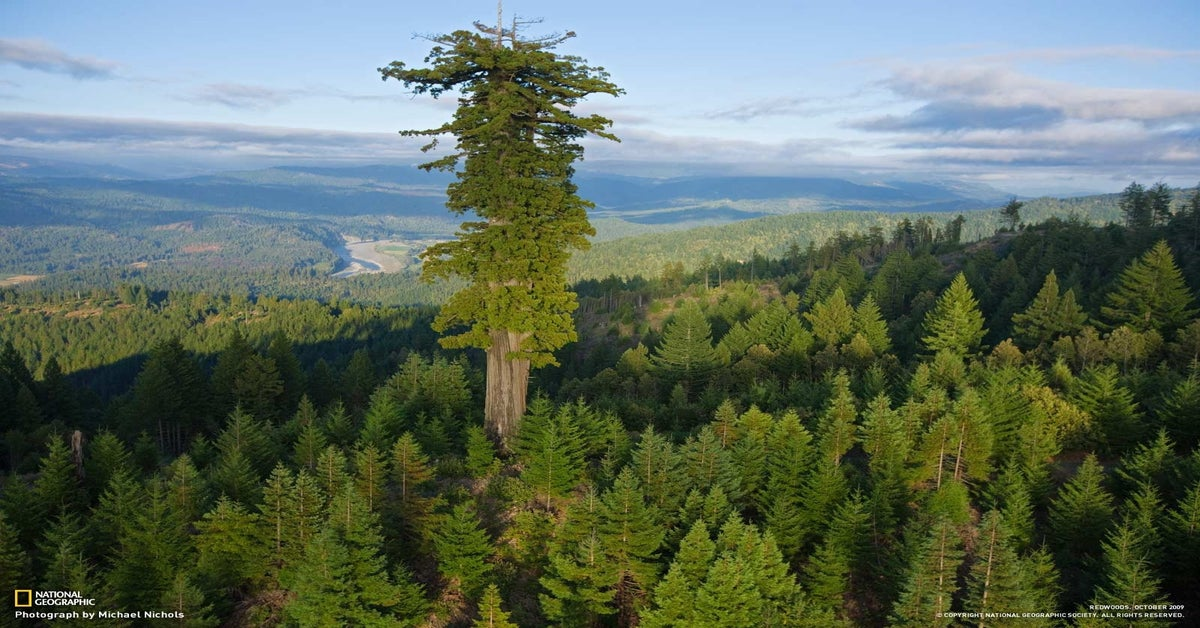
\includegraphics[max width=0.9\textwidth,max height=0.4\textheight]{{Images/hyperion}.jpg}
    \end{center}
    \end{column}
    \end{columns}
}
\end{frame}
    

\begin{frame}[t]{Round 5, Answer 8}
\vspace{0.5em}
\begin{block}{Question}
What kind of animal produces gossamer?
\end{block}
\visible<2->{
    \begin{columns}[T,totalwidth=\linewidth]
    \begin{column}{0.35\linewidth}
    \begin{block}{Answer}
    Spiders
    \end{block}
    \end{column}
    \begin{column}{0.6\linewidth}
    \begin{center}
    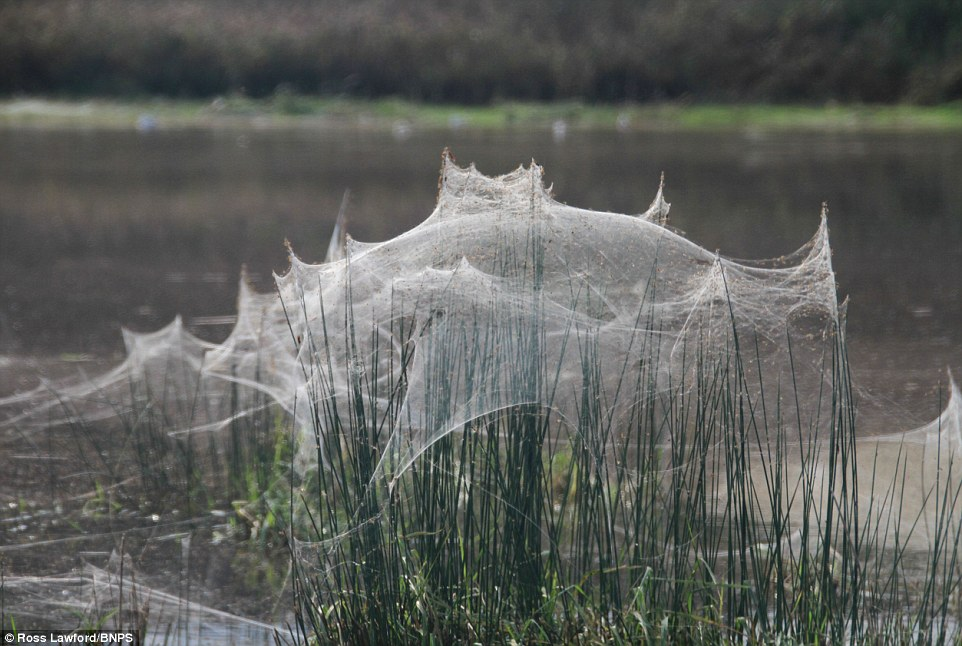
\includegraphics[max width=0.9\textwidth,max height=0.4\textheight]{{Images/gossamer}.jpg}
    \end{center}
    \end{column}
    \end{columns}
}
\end{frame}
    

\begin{frame}[t]{Round 5, Answer 9}
\vspace{0.5em}
\begin{block}{Question}
How many hearts does an octopus have?
\end{block}
\visible<2->{
    \begin{columns}[T,totalwidth=\linewidth]
    \begin{column}{0.35\linewidth}
    \begin{block}{Answer}
    Three
    \end{block}
    \end{column}
    \begin{column}{0.6\linewidth}
    \begin{center}
    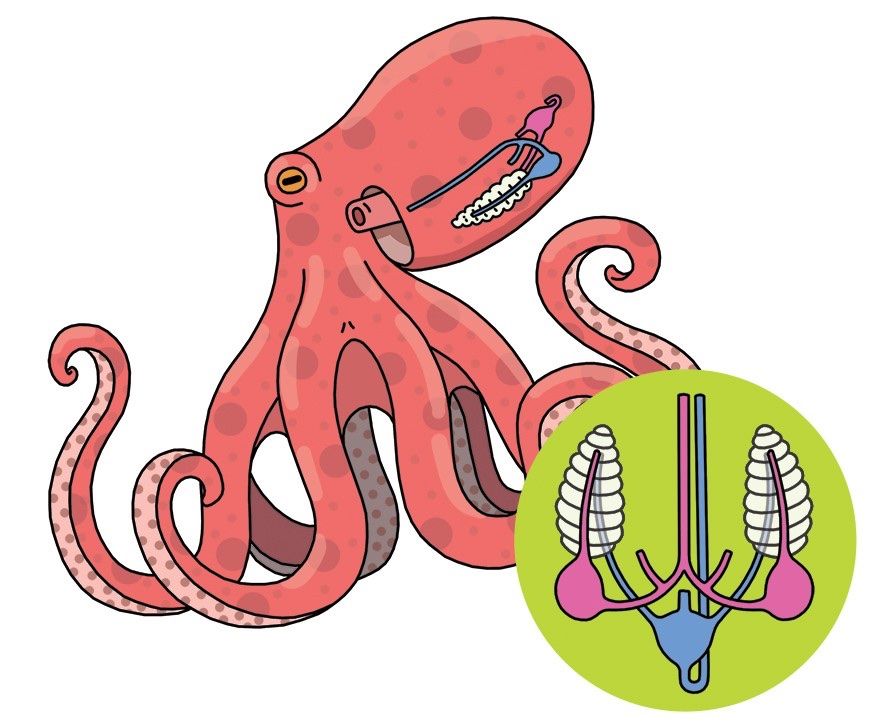
\includegraphics[max width=0.9\textwidth,max height=0.4\textheight]{{Images/octopus}.jpg}
    \end{center}
    \end{column}
    \end{columns}
}
\end{frame}
    

\begin{frame}[t]{Round 5, Answer 10}
\vspace{0.5em}
\begin{block}{Question}
The bark of which tree species is used to produce aspirin?
\end{block}
\visible<2->{
    \begin{columns}[T,totalwidth=\linewidth]
    \begin{column}{0.35\linewidth}
    \begin{block}{Answer}
    Willow tree
    \end{block}
    \end{column}
    \begin{column}{0.6\linewidth}
    \begin{center}
    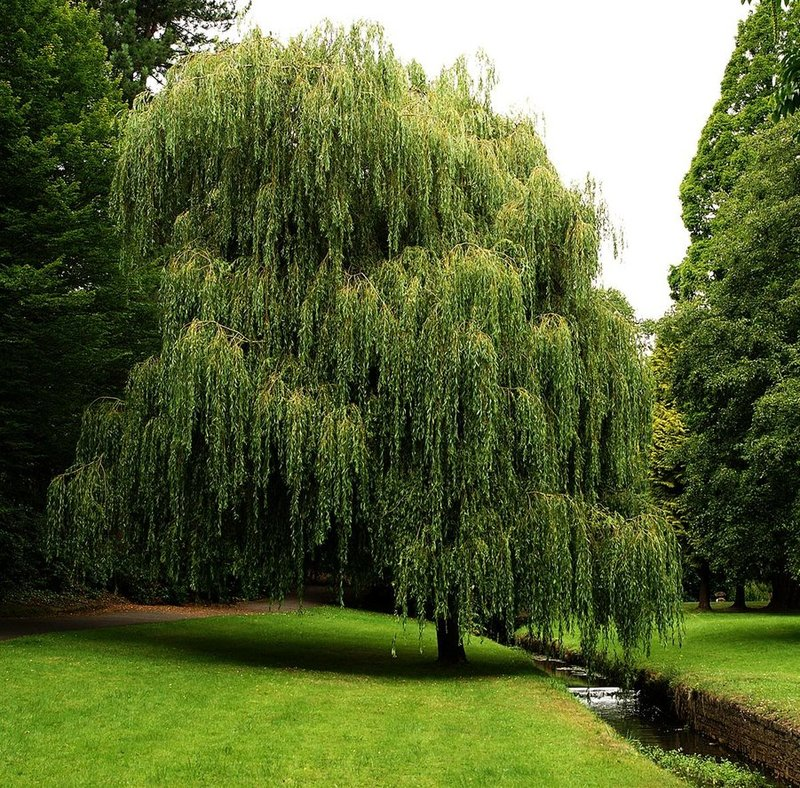
\includegraphics[max width=0.9\textwidth,max height=0.4\textheight]{{Images/willow}.jpg}
    \end{center}
    \end{column}
    \end{columns}
}
\end{frame}
    

\def\thisSectionName{Presidents}
\section{Round 6}
    

\subsection*{Q1}
\begin{frame}[t]{Round 6, Question 1}
\vspace{0.5em}
\begin{block}{Question}
Which president has an institute at Stanford University named after him?
\end{block}
\end{frame}
    

\subsection*{Q2}
\begin{frame}[t]{Round 6, Question 2}
\vspace{0.5em}
\begin{block}{Question}
In which speech did Lincoln say, ``With malice toward none, with charity for all, with firmness in the right as God gives us to see the right, let us strive on to finish the work we are in\ldots{}.''?
\end{block}
\end{frame}
    

\subsection*{Q3}
\begin{frame}[t]{Round 6, Question 3}
\vspace{0.5em}
\begin{block}{Question}
Which president immediately preceded Lincoln?
\end{block}
\end{frame}
    

\subsection*{Q4}
\begin{frame}[t]{Round 6, Question 4}
\vspace{0.5em}
\begin{block}{Question}
The capital of Liberia is named after which president?
\end{block}
\end{frame}
    

\subsection*{Q5}
\begin{frame}[t]{Round 6, Question 5}
\vspace{0.5em}
\begin{block}{Question}
Which president proposed an ``Alliance for Progress'' with Latin America?
\end{block}
\end{frame}
    

\subsection*{Q6}
\begin{frame}[t]{Round 6, Question 6}
\vspace{0.5em}
\begin{columns}[T,totalwidth=\linewidth]
\begin{column}{0.25\linewidth}
\begin{block}{Question}
What does the ``S'' in Harry S. Truman's name stand for?
\end{block}
\end{column}
\begin{column}{0.7\linewidth}
\begin{center}
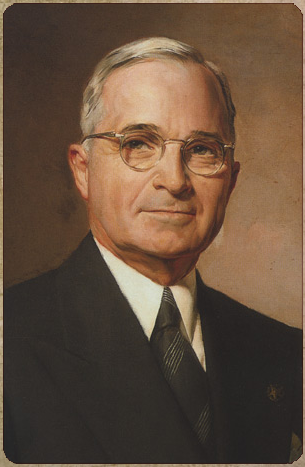
\includegraphics[max width=0.9\textwidth,max height=0.6\textheight]{{Images/truman}.png}
\end{center}
\end{column}
\end{columns}
\end{frame}
    

\subsection*{Q7}
\begin{frame}[t]{Round 6, Question 7}
\vspace{0.5em}
\begin{block}{Question}
Who was the youngest president to assume the presidency?
\end{block}
\end{frame}
    

\subsection*{Q8}
\begin{frame}[t]{Round 6, Question 8}
\vspace{0.5em}
\begin{block}{Question}
How many justices did President Obama appoint to the Supreme Court?
\end{block}
\end{frame}
    

\subsection*{Q9}
\begin{frame}[t]{Round 6, Question 9}
\vspace{0.5em}
\begin{block}{Question}
Who was the only U.S. President to also serve as Chief Justice of the Supreme Court? 
\end{block}
\end{frame}
    

\subsection*{Q10}
\begin{frame}[t]{Round 6, Question 10}
\vspace{0.5em}
\begin{block}{Question}
Which president proposed the League of Nations?
\end{block}
\end{frame}
    
\subsection{Answers}

\begin{frame}[t]{Round 6, Answer 1}
\vspace{0.5em}
\begin{block}{Question}
Which president has an institute at Stanford University named after him?
\end{block}
\visible<2->{
    \begin{columns}[T,totalwidth=\linewidth]
    \begin{column}{0.35\linewidth}
    \begin{block}{Answer}
    Herbert Hoover
    \end{block}
    \end{column}
    \begin{column}{0.6\linewidth}
    \begin{center}
    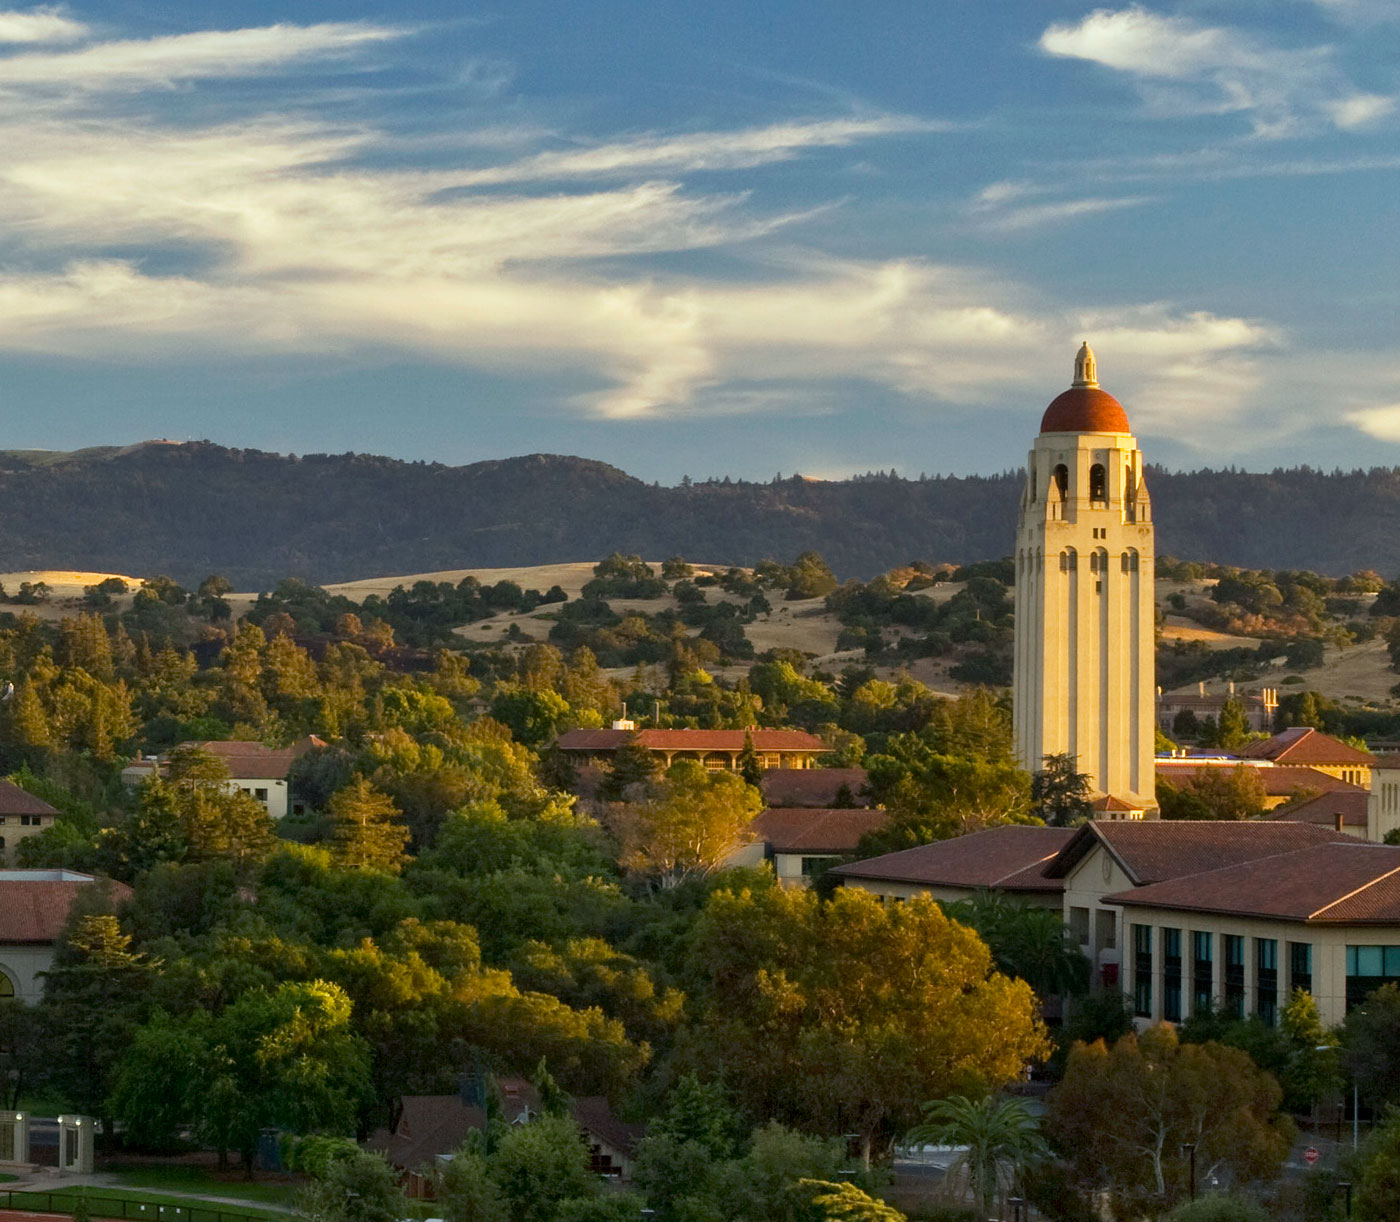
\includegraphics[max width=0.9\textwidth,max height=0.4\textheight]{{Images/hooverinst}.jpg}
    \end{center}
    \end{column}
    \end{columns}
}
\end{frame}
    

\begin{frame}[t]{Round 6, Answer 2}
\vspace{0.5em}
\begin{block}{Question}
In which speech did Lincoln say, ``With malice toward none, with charity for all, with firmness in the right as God gives us to see the right, let us strive on to finish the work we are in\ldots{}.''?
\end{block}
\visible<2->{
    \begin{columns}[T,totalwidth=\linewidth]
    \begin{column}{0.35\linewidth}
    \begin{block}{Answer}
    His Second Inaugural Address
    \end{block}
    \end{column}
    \begin{column}{0.6\linewidth}
    \begin{center}
    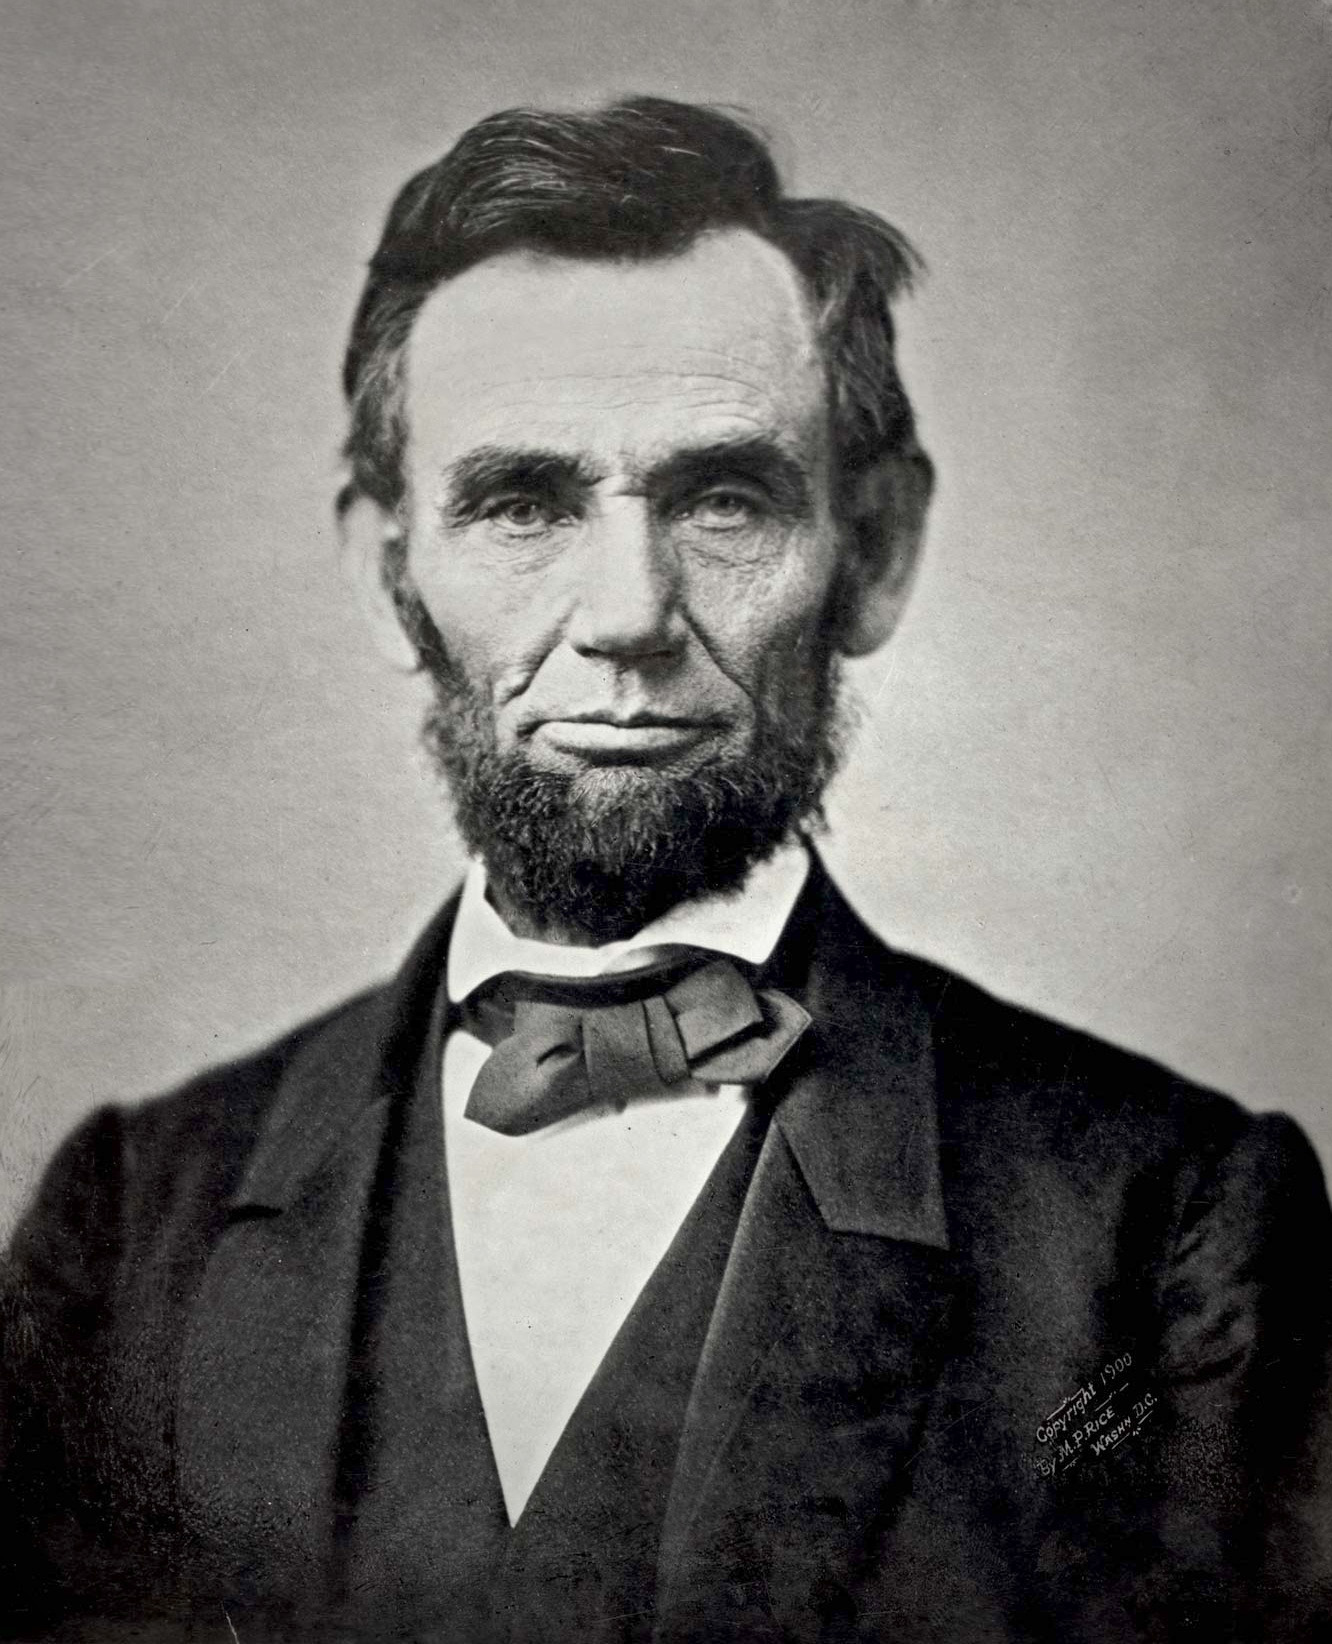
\includegraphics[max width=0.9\textwidth,max height=0.4\textheight]{{Images/lincoln}.jpeg}
    \end{center}
    \end{column}
    \end{columns}
}
\end{frame}
    

\begin{frame}[t]{Round 6, Answer 3}
\vspace{0.5em}
\begin{block}{Question}
Which president immediately preceded Lincoln?
\end{block}
\visible<2->{
    \begin{columns}[T,totalwidth=\linewidth]
    \begin{column}{0.35\linewidth}
    \begin{block}{Answer}
    James Buchanan
    \end{block}
    \end{column}
    \begin{column}{0.6\linewidth}
    \begin{center}
    \includegraphics[max width=0.9\textwidth,max height=0.4\textheight]{{Images/buchanan}.jpg}
    \end{center}
    \end{column}
    \end{columns}
}
\end{frame}
    

\begin{frame}[t]{Round 6, Answer 4}
\vspace{0.5em}
\begin{block}{Question}
The capital of Liberia is named after which president?
\end{block}
\visible<2->{
    \begin{columns}[T,totalwidth=\linewidth]
    \begin{column}{0.35\linewidth}
    \begin{block}{Answer}
    James Monroe (Monrovia)
    \end{block}
    \end{column}
    \begin{column}{0.6\linewidth}
    \begin{center}
    \includegraphics[max width=0.9\textwidth,max height=0.4\textheight]{{Images/monrovia}.jpg}
    \end{center}
    \end{column}
    \end{columns}
}
\end{frame}
    

\begin{frame}[t]{Round 6, Answer 5}
\vspace{0.5em}
\begin{block}{Question}
Which president proposed an ``Alliance for Progress'' with Latin America?
\end{block}
\visible<2->{
    \begin{columns}[T,totalwidth=\linewidth]
    \begin{column}{0.35\linewidth}
    \begin{block}{Answer}
    John F. Kennedy
    \end{block}
    \end{column}
    \begin{column}{0.6\linewidth}
    \begin{center}
    \includegraphics[max width=0.9\textwidth,max height=0.4\textheight]{{Images/jfks-alliance-for-progress}.jpg}
    \end{center}
    \end{column}
    \end{columns}
}
\end{frame}
    

\begin{frame}[t]{Round 6, Answer 6}
\vspace{0.5em}
\begin{columns}[T,totalwidth=\linewidth]
\begin{column}{0.35\linewidth}
\begin{block}{Question}
What does the ``S'' in Harry S. Truman's name stand for?
\end{block}
\visible<2->{
    \begin{block}{Answer}
    Nothing — he did not have a middle name
    \end{block}
}
\end{column}
\begin{column}{0.6\linewidth}
\begin{center}
\includegraphics[max width=0.9\textwidth,max height=0.6\textheight]{{Images/truman}.png}
\end{center}
\end{column}
\end{columns}
\end{frame}
    

\begin{frame}[t]{Round 6, Answer 7}
\vspace{0.5em}
\begin{block}{Question}
Who was the youngest president to assume the presidency?
\end{block}
\visible<2->{
    \begin{columns}[T,totalwidth=\linewidth]
    \begin{column}{0.35\linewidth}
    \begin{block}{Answer}
    Teddy Roosevelt (42 years, 322 days)
    \end{block}
    \end{column}
    \begin{column}{0.6\linewidth}
    \begin{center}
    \includegraphics[max width=0.9\textwidth,max height=0.4\textheight]{{Images/tr}.png}
    \end{center}
    \end{column}
    \end{columns}
}
\end{frame}
    

\begin{frame}[t]{Round 6, Answer 8}
\vspace{0.5em}
\begin{block}{Question}
How many justices did President Obama appoint to the Supreme Court?
\end{block}
\visible<2->{
    \begin{columns}[T,totalwidth=\linewidth]
    \begin{column}{0.35\linewidth}
    \begin{block}{Answer}
    Two: Sonia Sotomayor and Elena Kagan
    \end{block}
    \end{column}
    \begin{column}{0.6\linewidth}
    \begin{center}
    \includegraphics[max width=0.9\textwidth,max height=0.4\textheight]{{Images/justices}.jpg}
    \end{center}
    \end{column}
    \end{columns}
}
\end{frame}
    

\begin{frame}[t]{Round 6, Answer 9}
\vspace{0.5em}
\begin{block}{Question}
Who was the only U.S. President to also serve as Chief Justice of the Supreme Court? 
\end{block}
\visible<2->{
    \begin{columns}[T,totalwidth=\linewidth]
    \begin{column}{0.35\linewidth}
    \begin{block}{Answer}
    William Howard Taft
    \end{block}
    \end{column}
    \begin{column}{0.6\linewidth}
    \begin{center}
    \includegraphics[max width=0.9\textwidth,max height=0.4\textheight]{{Images/taft}.jpg}
    \end{center}
    \end{column}
    \end{columns}
}
\end{frame}
    

\begin{frame}[t]{Round 6, Answer 10}
\vspace{0.5em}
\begin{block}{Question}
Which president proposed the League of Nations?
\end{block}
\visible<2->{
    \begin{columns}[T,totalwidth=\linewidth]
    \begin{column}{0.35\linewidth}
    \begin{block}{Answer}
    Woodrow Wilson
    \end{block}
    \end{column}
    \begin{column}{0.6\linewidth}
    \begin{center}
    \includegraphics[max width=0.9\textwidth,max height=0.4\textheight]{{Images/wilson}.jpg}
    \end{center}
    \end{column}
    \end{columns}
}
\end{frame}
    

\def\thisSectionName{Dr.\ Anthony S.\ Fauci: Great New Yorker and Great Italian-American}
\section{Round 7}
    

\subsection*{Q1}
\begin{frame}[t]{Round 7, Question 1}
\vspace{0.5em}
\begin{block}{Question}
How many children does Dr.\ Fauci have?
\end{block}
\end{frame}
    

\subsection*{Q2}
\begin{frame}[t]{Round 7, Question 2}
\vspace{0.5em}
\begin{block}{Question}
How old is Dr.\ Fauci?
\end{block}
\end{frame}
    

\subsection*{Q3}
\begin{frame}[t]{Round 7, Question 3}
\vspace{0.5em}
\begin{block}{Question}
In high school, Dr.\ Fauci was captain of a team in which sport?
\end{block}
\end{frame}
    

\subsection*{Q4}
\begin{frame}[t]{Round 7, Question 4}
\vspace{0.5em}
\begin{block}{Question}
In which New York City borough was Dr.\ Fauci born?
\end{block}
\end{frame}
    

\subsection*{Q5}
\begin{frame}[t]{Round 7, Question 5}
\vspace{0.5em}
\begin{block}{Question}
What medical school did Dr.\ Fauci attend?
\end{block}
\end{frame}
    

\subsection*{Q6}
\begin{frame}[t]{Round 7, Question 6}
\vspace{0.5em}
\begin{block}{Question}
What college did Dr.\ Fauci attend?
\end{block}
\end{frame}
    

\subsection*{Q7}
\begin{frame}[t]{Round 7, Question 7}
\vspace{0.5em}
\begin{block}{Question}
What high school did Dr.\ Fauci attend?
\end{block}
\end{frame}
    

\subsection*{Q8}
\begin{frame}[t]{Round 7, Question 8}
\vspace{0.5em}
\begin{block}{Question}
What is Dr.\ Anthony S. Fauci's middle name?
\end{block}
\end{frame}
    

\subsection*{Q9}
\begin{frame}[t]{Round 7, Question 9}
\vspace{0.5em}
\begin{block}{Question}
What is Dr.\ Fauci's favorite novel?
\end{block}
\end{frame}
    

\subsection*{Q10}
\begin{frame}[t]{Round 7, Question 10}
\vspace{0.5em}
\begin{block}{Question}
What high honor did Dr.\ Fauci receive in 2008?
\end{block}
\end{frame}
    
\subsection{Answers}

\begin{frame}[t]{Round 7, Answer 1}
\vspace{0.5em}
\begin{block}{Question}
How many children does Dr.\ Fauci have?
\end{block}
\visible<2->{
    \begin{columns}[T,totalwidth=\linewidth]
    \begin{column}{0.35\linewidth}
    \begin{block}{Answer}
    3
    \end{block}
    \end{column}
    \begin{column}{0.6\linewidth}
    \begin{center}
    \includegraphics[max width=0.9\textwidth,max height=0.4\textheight]{{Images/faucichildren}.jpg}
    \end{center}
    \end{column}
    \end{columns}
}
\end{frame}
    

\begin{frame}[t]{Round 7, Answer 2}
\vspace{0.5em}
\begin{block}{Question}
How old is Dr.\ Fauci?
\end{block}
\visible<2->{
    \begin{columns}[T,totalwidth=\linewidth]
    \begin{column}{0.35\linewidth}
    \begin{block}{Answer}
    79
    \end{block}
    \end{column}
    \begin{column}{0.6\linewidth}
    \begin{center}
    \includegraphics[max width=0.9\textwidth,max height=0.4\textheight]{{Images/fauciage}.jpg}
    \end{center}
    \end{column}
    \end{columns}
}
\end{frame}
    

\begin{frame}[t]{Round 7, Answer 3}
\vspace{0.5em}
\begin{block}{Question}
In high school, Dr.\ Fauci was captain of a team in which sport?
\end{block}
\visible<2->{
    \begin{columns}[T,totalwidth=\linewidth]
    \begin{column}{0.35\linewidth}
    \begin{block}{Answer}
    Basketball
    \end{block}
    \end{column}
    \begin{column}{0.6\linewidth}
    \begin{center}
    \includegraphics[max width=0.9\textwidth,max height=0.4\textheight]{{Images/faucibasketball}.jpg}
    \end{center}
    \end{column}
    \end{columns}
}
\end{frame}
    

\begin{frame}[t]{Round 7, Answer 4}
\vspace{0.5em}
\begin{block}{Question}
In which New York City borough was Dr.\ Fauci born?
\end{block}
\visible<2->{
    \begin{columns}[T,totalwidth=\linewidth]
    \begin{column}{0.35\linewidth}
    \begin{block}{Answer}
    Brooklyn
    \end{block}
    \end{column}
    \begin{column}{0.6\linewidth}
    \begin{center}
    \includegraphics[max width=0.9\textwidth,max height=0.4\textheight]{{Images/faucichild}.jpg}
    \end{center}
    \end{column}
    \end{columns}
}
\end{frame}
    

\begin{frame}[t]{Round 7, Answer 5}
\vspace{0.5em}
\begin{block}{Question}
What medical school did Dr.\ Fauci attend?
\end{block}
\visible<2->{
    \begin{columns}[T,totalwidth=\linewidth]
    \begin{column}{0.35\linewidth}
    \begin{block}{Answer}
    Cornell
    \end{block}
    \end{column}
    \begin{column}{0.6\linewidth}
    \begin{center}
    \includegraphics[max width=0.9\textwidth,max height=0.4\textheight]{{Images/faucicornell}.jpg}
    \end{center}
    \end{column}
    \end{columns}
}
\end{frame}
    

\begin{frame}[t]{Round 7, Answer 6}
\vspace{0.5em}
\begin{block}{Question}
What college did Dr.\ Fauci attend?
\end{block}
\visible<2->{
    \begin{columns}[T,totalwidth=\linewidth]
    \begin{column}{0.35\linewidth}
    \begin{block}{Answer}
    Holy Cross
    \end{block}
    \end{column}
    \begin{column}{0.6\linewidth}
    \begin{center}
    \includegraphics[max width=0.9\textwidth,max height=0.4\textheight]{{Images/holycross}.png}
    \end{center}
    \end{column}
    \end{columns}
}
\end{frame}
    

\begin{frame}[t]{Round 7, Answer 7}
\vspace{0.5em}
\begin{block}{Question}
What high school did Dr.\ Fauci attend?
\end{block}
\visible<2->{
    \begin{columns}[T,totalwidth=\linewidth]
    \begin{column}{0.35\linewidth}
    \begin{block}{Answer}
    Regis
    \end{block}
    \end{column}
    \begin{column}{0.6\linewidth}
    \begin{center}
    \includegraphics[max width=0.9\textwidth,max height=0.4\textheight]{{Images/regis}.jpeg}
    \end{center}
    \end{column}
    \end{columns}
}
\end{frame}
    

\begin{frame}[t]{Round 7, Answer 8}
\vspace{0.5em}
\begin{block}{Question}
What is Dr.\ Anthony S. Fauci's middle name?
\end{block}
\visible<2->{
    \begin{block}{Answer}
    Stephen
    \end{block}
}
\end{frame}
    

\begin{frame}[t]{Round 7, Answer 9}
\vspace{0.5em}
\begin{block}{Question}
What is Dr.\ Fauci's favorite novel?
\end{block}
\visible<2->{
    \begin{columns}[T,totalwidth=\linewidth]
    \begin{column}{0.35\linewidth}
    \begin{block}{Answer}
    The Godfather
    \end{block}
    \end{column}
    \begin{column}{0.6\linewidth}
    \begin{center}
    \includegraphics[max width=0.9\textwidth,max height=0.4\textheight]{{Images/faucigodfather}.jpg}
    \end{center}
    \end{column}
    \end{columns}
}
\end{frame}
    

\begin{frame}[t]{Round 7, Answer 10}
\vspace{0.5em}
\begin{block}{Question}
What high honor did Dr.\ Fauci receive in 2008?
\end{block}
\visible<2->{
    \begin{columns}[T,totalwidth=\linewidth]
    \begin{column}{0.35\linewidth}
    \begin{block}{Answer}
    The Medal of Freedom
    \end{block}
    \end{column}
    \begin{column}{0.6\linewidth}
    \begin{center}
    \includegraphics[max width=0.9\textwidth,max height=0.4\textheight]{{Images/faucimof}.jpeg}
    \end{center}
    \end{column}
    \end{columns}
}
\end{frame}
    

\def\thisSectionName{Famous Paintings}
\section{Round 8}
    

\subsection*{Q1}
\begin{frame}[t]{Round 8, Question 1}
\vspace{0.5em}
\begin{columns}[T,totalwidth=\linewidth]
\begin{column}{0.25\linewidth}
\begin{block}{Question}
Name the painter.
\end{block}
\end{column}
\begin{column}{0.7\linewidth}
\begin{center}
\includegraphics[max width=0.9\textwidth,max height=0.6\textheight]{{Images/monet}.jpg}
\end{center}
\end{column}
\end{columns}
\end{frame}
    

\subsection*{Q2}
\begin{frame}[t]{Round 8, Question 2}
\vspace{0.5em}
\begin{columns}[T,totalwidth=\linewidth]
\begin{column}{0.25\linewidth}
\begin{block}{Question}
Name the painter.
\end{block}
\end{column}
\begin{column}{0.7\linewidth}
\begin{center}
\includegraphics[max width=0.9\textwidth,max height=0.6\textheight]{{Images/hockney}.jpg}
\end{center}
\end{column}
\end{columns}
\end{frame}
    

\subsection*{Q3}
\begin{frame}[t]{Round 8, Question 3}
\vspace{0.5em}
\begin{columns}[T,totalwidth=\linewidth]
\begin{column}{0.25\linewidth}
\begin{block}{Question}
Name the painter.
\end{block}
\end{column}
\begin{column}{0.7\linewidth}
\begin{center}
\includegraphics[max width=0.9\textwidth,max height=0.6\textheight]{{Images/velasquez}.jpg}
\end{center}
\end{column}
\end{columns}
\end{frame}
    

\subsection*{Q4}
\begin{frame}[t]{Round 8, Question 4}
\vspace{0.5em}
\begin{columns}[T,totalwidth=\linewidth]
\begin{column}{0.25\linewidth}
\begin{block}{Question}
Name the painter.
\end{block}
\end{column}
\begin{column}{0.7\linewidth}
\begin{center}
\includegraphics[max width=0.9\textwidth,max height=0.6\textheight]{{Images/churchniagara}.jpg}
\end{center}
\end{column}
\end{columns}
\end{frame}
    

\subsection*{Q5}
\begin{frame}[t]{Round 8, Question 5}
\vspace{0.5em}
\begin{columns}[T,totalwidth=\linewidth]
\begin{column}{0.25\linewidth}
\begin{block}{Question}
Name the painter.
\end{block}
\end{column}
\begin{column}{0.7\linewidth}
\begin{center}
\includegraphics[max width=0.9\textwidth,max height=0.6\textheight]{{Images/giotto}.jpg}
\end{center}
\end{column}
\end{columns}
\end{frame}
    

\subsection*{Q6}
\begin{frame}[t]{Round 8, Question 6}
\vspace{0.5em}
\begin{columns}[T,totalwidth=\linewidth]
\begin{column}{0.25\linewidth}
\begin{block}{Question}
Name the painter.
\end{block}
\end{column}
\begin{column}{0.7\linewidth}
\begin{center}
\includegraphics[max width=0.9\textwidth,max height=0.6\textheight]{{Images/jacoblawrence}.jpg}
\end{center}
\end{column}
\end{columns}
\end{frame}
    

\subsection*{Q7}
\begin{frame}[t]{Round 8, Question 7}
\vspace{0.5em}
\begin{columns}[T,totalwidth=\linewidth]
\begin{column}{0.25\linewidth}
\begin{block}{Question}
Name the painter.
\end{block}
\end{column}
\begin{column}{0.7\linewidth}
\begin{center}
\includegraphics[max width=0.9\textwidth,max height=0.6\textheight]{{Images/sorolla}.jpg}
\end{center}
\end{column}
\end{columns}
\end{frame}
    

\subsection*{Q8}
\begin{frame}[t]{Round 8, Question 8}
\vspace{0.5em}
\begin{columns}[T,totalwidth=\linewidth]
\begin{column}{0.25\linewidth}
\begin{block}{Question}
Name the painter.
\end{block}
\end{column}
\begin{column}{0.7\linewidth}
\begin{center}
\includegraphics[max width=0.9\textwidth,max height=0.6\textheight]{{Images/american-gothic}.jpg}
\end{center}
\end{column}
\end{columns}
\end{frame}
    

\subsection*{Q9}
\begin{frame}[t]{Round 8, Question 9}
\vspace{0.5em}
\begin{columns}[T,totalwidth=\linewidth]
\begin{column}{0.25\linewidth}
\begin{block}{Question}
Name the painter.
\end{block}
\end{column}
\begin{column}{0.7\linewidth}
\begin{center}
\includegraphics[max width=0.9\textwidth,max height=0.6\textheight]{{Images/guernica}.jpg}
\end{center}
\end{column}
\end{columns}
\end{frame}
    

\subsection*{Q10}
\begin{frame}[t]{Round 8, Question 10}
\vspace{0.5em}
\begin{columns}[T,totalwidth=\linewidth]
\begin{column}{0.25\linewidth}
\begin{block}{Question}
Name the painter.
\end{block}
\end{column}
\begin{column}{0.7\linewidth}
\begin{center}
\includegraphics[max width=0.9\textwidth,max height=0.6\textheight]{{Images/rothko}.jpg}
\end{center}
\end{column}
\end{columns}
\end{frame}
    
\subsection{Answers}

\begin{frame}[t]{Round 8, Answer 1}
\vspace{0.5em}
\begin{columns}[T,totalwidth=\linewidth]
\begin{column}{0.35\linewidth}
\begin{block}{Question}
Name the painter.
\end{block}
\visible<2->{
    \begin{block}{Answer}
    Claude Monet (\emph{Rouen Cathedral})
    \end{block}
}
\end{column}
\begin{column}{0.6\linewidth}
\begin{center}
\includegraphics[max width=0.9\textwidth,max height=0.6\textheight]{{Images/monet}.jpg}
\end{center}
\end{column}
\end{columns}
\end{frame}
    

\begin{frame}[t]{Round 8, Answer 2}
\vspace{0.5em}
\begin{columns}[T,totalwidth=\linewidth]
\begin{column}{0.35\linewidth}
\begin{block}{Question}
Name the painter.
\end{block}
\visible<2->{
    \begin{block}{Answer}
    David Hockney (\emph{A Bigger Splash})
    \end{block}
}
\end{column}
\begin{column}{0.6\linewidth}
\begin{center}
\includegraphics[max width=0.9\textwidth,max height=0.6\textheight]{{Images/hockney}.jpg}
\end{center}
\end{column}
\end{columns}
\end{frame}
    

\begin{frame}[t]{Round 8, Answer 3}
\vspace{0.5em}
\begin{columns}[T,totalwidth=\linewidth]
\begin{column}{0.35\linewidth}
\begin{block}{Question}
Name the painter.
\end{block}
\visible<2->{
    \begin{block}{Answer}
    Diego Velasquez (\emph{Las Meninas})
    \end{block}
}
\end{column}
\begin{column}{0.6\linewidth}
\begin{center}
\includegraphics[max width=0.9\textwidth,max height=0.6\textheight]{{Images/velasquez}.jpg}
\end{center}
\end{column}
\end{columns}
\end{frame}
    

\begin{frame}[t]{Round 8, Answer 4}
\vspace{0.5em}
\begin{columns}[T,totalwidth=\linewidth]
\begin{column}{0.35\linewidth}
\begin{block}{Question}
Name the painter.
\end{block}
\visible<2->{
    \begin{block}{Answer}
    Frederic Edwin Church (\emph{Niagara})
    \end{block}
}
\end{column}
\begin{column}{0.6\linewidth}
\begin{center}
\includegraphics[max width=0.9\textwidth,max height=0.6\textheight]{{Images/churchniagara}.jpg}
\end{center}
\end{column}
\end{columns}
\end{frame}
    

\begin{frame}[t]{Round 8, Answer 5}
\vspace{0.5em}
\begin{columns}[T,totalwidth=\linewidth]
\begin{column}{0.35\linewidth}
\begin{block}{Question}
Name the painter.
\end{block}
\visible<2->{
    \begin{block}{Answer}
    Giotto (\emph{The Death of St.\ Francis})
    \end{block}
}
\end{column}
\begin{column}{0.6\linewidth}
\begin{center}
\includegraphics[max width=0.9\textwidth,max height=0.6\textheight]{{Images/giotto}.jpg}
\end{center}
\end{column}
\end{columns}
\end{frame}
    

\begin{frame}[t]{Round 8, Answer 6}
\vspace{0.5em}
\begin{columns}[T,totalwidth=\linewidth]
\begin{column}{0.35\linewidth}
\begin{block}{Question}
Name the painter.
\end{block}
\visible<2->{
    \begin{block}{Answer}
    Jacob Lawrence (from the \emph{Great Migration} series)
    \end{block}
}
\end{column}
\begin{column}{0.6\linewidth}
\begin{center}
\includegraphics[max width=0.9\textwidth,max height=0.6\textheight]{{Images/jacoblawrence}.jpg}
\end{center}
\end{column}
\end{columns}
\end{frame}
    

\begin{frame}[t]{Round 8, Answer 7}
\vspace{0.5em}
\begin{columns}[T,totalwidth=\linewidth]
\begin{column}{0.35\linewidth}
\begin{block}{Question}
Name the painter.
\end{block}
\visible<2->{
    \begin{block}{Answer}
    Joaquin Sorolla (\emph{Walk on the Beach})
    \end{block}
}
\end{column}
\begin{column}{0.6\linewidth}
\begin{center}
\includegraphics[max width=0.9\textwidth,max height=0.6\textheight]{{Images/sorolla}.jpg}
\end{center}
\end{column}
\end{columns}
\end{frame}
    

\begin{frame}[t]{Round 8, Answer 8}
\vspace{0.5em}
\begin{columns}[T,totalwidth=\linewidth]
\begin{column}{0.35\linewidth}
\begin{block}{Question}
Name the painter.
\end{block}
\visible<2->{
    \begin{block}{Answer}
    Grant Wood (\emph{American Gothic} — updated)
    \end{block}
}
\end{column}
\begin{column}{0.6\linewidth}
\begin{center}
\includegraphics[max width=0.9\textwidth,max height=0.6\textheight]{{Images/american-gothic}.jpg}
\end{center}
\end{column}
\end{columns}
\end{frame}
    

\begin{frame}[t]{Round 8, Answer 9}
\vspace{0.5em}
\begin{columns}[T,totalwidth=\linewidth]
\begin{column}{0.35\linewidth}
\begin{block}{Question}
Name the painter.
\end{block}
\visible<2->{
    \begin{block}{Answer}
    Pablo Picasso (\emph{Guernica})
    \end{block}
}
\end{column}
\begin{column}{0.6\linewidth}
\begin{center}
\includegraphics[max width=0.9\textwidth,max height=0.6\textheight]{{Images/guernica}.jpg}
\end{center}
\end{column}
\end{columns}
\end{frame}
    

\begin{frame}[t]{Round 8, Answer 10}
\vspace{0.5em}
\begin{columns}[T,totalwidth=\linewidth]
\begin{column}{0.35\linewidth}
\begin{block}{Question}
Name the painter.
\end{block}
\visible<2->{
    \begin{block}{Answer}
    Mark Rothko (\emph{White Over Red})
    \end{block}
}
\end{column}
\begin{column}{0.6\linewidth}
\begin{center}
\includegraphics[max width=0.9\textwidth,max height=0.6\textheight]{{Images/rothko}.jpg}
\end{center}
\end{column}
\end{columns}
\end{frame}
    

\def\thisSectionName{Canada --- Our Friendly Neighbor to the North}
\section{Round 9}
    

\subsection*{Q1}
\begin{frame}[t]{Round 9, Question 1}
\vspace{0.5em}
\begin{block}{Question}
Canada is the world's largest exporter of what fruit?
\end{block}
\end{frame}
    

\subsection*{Q2}
\begin{frame}[t]{Round 9, Question 2}
\vspace{0.5em}
\begin{block}{Question}
Which Canadian city is home to North America's largest shopping mall?
\end{block}
\end{frame}
    

\subsection*{Q3}
\begin{frame}[t]{Round 9, Question 3}
\vspace{0.5em}
\begin{block}{Question}
Not including the stem, how many points are on the maple leaf on Canada's flag?
\end{block}
\end{frame}
    

\subsection*{Q4}
\begin{frame}[t]{Round 9, Question 4}
\vspace{0.5em}
\begin{block}{Question}
What is Canada's national sport?
\end{block}
\end{frame}
    

\subsection*{Q5}
\begin{frame}[t]{Round 9, Question 5}
\vspace{0.5em}
\begin{block}{Question}
Which city in Canada has the most restaurants per capita?
\end{block}
\end{frame}
    

\subsection*{Q6}
\begin{frame}[t]{Round 9, Question 6}
\vspace{0.5em}
\begin{block}{Question}
What is the name of the highest peak in Canada?
\end{block}
\end{frame}
    

\subsection*{Q7}
\begin{frame}[t]{Round 9, Question 7}
\vspace{0.5em}
\begin{block}{Question}
Cirque du Soleil originated in which Canadian province?
\end{block}
\end{frame}
    

\subsection*{Q8}
\begin{frame}[t]{Round 9, Question 8}
\vspace{0.5em}
\begin{block}{Question}
How many time zones does Canada have?
\end{block}
\end{frame}
    

\subsection*{Q9}
\begin{frame}[t]{Round 9, Question 9}
\vspace{0.5em}
\begin{block}{Question}
What is Canada's oldest city?
\end{block}
\end{frame}
    

\subsection*{Q10}
\begin{frame}[t]{Round 9, Question 10}
\vspace{0.5em}
\begin{block}{Question}
Which famous Canadian restaurant chain opened in Hamilton in 1964?
\end{block}
\end{frame}
    
\subsection{Answers}

\begin{frame}[t]{Round 9, Answer 1}
\vspace{0.5em}
\begin{block}{Question}
Canada is the world's largest exporter of what fruit?
\end{block}
\visible<2->{
    \begin{columns}[T,totalwidth=\linewidth]
    \begin{column}{0.35\linewidth}
    \begin{block}{Answer}
    Blueberries
    \end{block}
    \end{column}
    \begin{column}{0.6\linewidth}
    \begin{center}
    \includegraphics[max width=0.9\textwidth,max height=0.4\textheight]{{Images/blueberry-cultivation-in-himachal}.jpg}
    \end{center}
    \end{column}
    \end{columns}
}
\end{frame}
    

\begin{frame}[t]{Round 9, Answer 2}
\vspace{0.5em}
\begin{block}{Question}
Which Canadian city is home to North America's largest shopping mall?
\end{block}
\visible<2->{
    \begin{columns}[T,totalwidth=\linewidth]
    \begin{column}{0.35\linewidth}
    \begin{block}{Answer}
    Edmonton, Alberta (The West Edmonton Mall)
    \end{block}
    \end{column}
    \begin{column}{0.6\linewidth}
    \begin{center}
    \includegraphics[max width=0.9\textwidth,max height=0.4\textheight]{{Images/West-Edmonton-Mall-33924}.jpg}
    \end{center}
    \end{column}
    \end{columns}
}
\end{frame}
    

\begin{frame}[t]{Round 9, Answer 3}
\vspace{0.5em}
\begin{block}{Question}
Not including the stem, how many points are on the maple leaf on Canada's flag?
\end{block}
\visible<2->{
    \begin{columns}[T,totalwidth=\linewidth]
    \begin{column}{0.35\linewidth}
    \begin{block}{Answer}
    Eleven
    \end{block}
    \end{column}
    \begin{column}{0.6\linewidth}
    \begin{center}
    \includegraphics[max width=0.9\textwidth,max height=0.4\textheight]{{Images/canada}.png}
    \end{center}
    \end{column}
    \end{columns}
}
\end{frame}
    

\begin{frame}[t]{Round 9, Answer 4}
\vspace{0.5em}
\begin{block}{Question}
What is Canada's national sport?
\end{block}
\visible<2->{
    \begin{columns}[T,totalwidth=\linewidth]
    \begin{column}{0.35\linewidth}
    \begin{block}{Answer}
    Lacrosse
    \end{block}
    \end{column}
    \begin{column}{0.6\linewidth}
    \begin{center}
    \includegraphics[max width=0.9\textwidth,max height=0.4\textheight]{{Images/lacrosse}.jpg}
    \end{center}
    \end{column}
    \end{columns}
}
\end{frame}
    

\begin{frame}[t]{Round 9, Answer 5}
\vspace{0.5em}
\begin{block}{Question}
Which city in Canada has the most restaurants per capita?
\end{block}
\visible<2->{
    \begin{columns}[T,totalwidth=\linewidth]
    \begin{column}{0.35\linewidth}
    \begin{block}{Answer}
    Montreal
    \end{block}
    \end{column}
    \begin{column}{0.6\linewidth}
    \begin{center}
    \includegraphics[max width=0.9\textwidth,max height=0.4\textheight]{{Images/Montreal-Canada}.jpg}
    \end{center}
    \end{column}
    \end{columns}
}
\end{frame}
    

\begin{frame}[t]{Round 9, Answer 6}
\vspace{0.5em}
\begin{block}{Question}
What is the name of the highest peak in Canada?
\end{block}
\visible<2->{
    \begin{columns}[T,totalwidth=\linewidth]
    \begin{column}{0.35\linewidth}
    \begin{block}{Answer}
    Mount Logan (5,959 meters)
    \end{block}
    \end{column}
    \begin{column}{0.6\linewidth}
    \begin{center}
    \includegraphics[max width=0.9\textwidth,max height=0.4\textheight]{{Images/logan}.jpg}
    \end{center}
    \end{column}
    \end{columns}
}
\end{frame}
    

\begin{frame}[t]{Round 9, Answer 7}
\vspace{0.5em}
\begin{block}{Question}
Cirque du Soleil originated in which Canadian province?
\end{block}
\visible<2->{
    \begin{columns}[T,totalwidth=\linewidth]
    \begin{column}{0.35\linewidth}
    \begin{block}{Answer}
    Quebec
    \end{block}
    \end{column}
    \begin{column}{0.6\linewidth}
    \begin{center}
    \includegraphics[max width=0.9\textwidth,max height=0.4\textheight]{{Images/cirque}.jpeg}
    \end{center}
    \end{column}
    \end{columns}
}
\end{frame}
    

\begin{frame}[t]{Round 9, Answer 8}
\vspace{0.5em}
\begin{block}{Question}
How many time zones does Canada have?
\end{block}
\visible<2->{
    \begin{columns}[T,totalwidth=\linewidth]
    \begin{column}{0.35\linewidth}
    \begin{block}{Answer}
    Six
    \end{block}
    \end{column}
    \begin{column}{0.6\linewidth}
    \begin{center}
    \includegraphics[max width=0.9\textwidth,max height=0.4\textheight]{{Images/canadatimezones}.png}
    \end{center}
    \end{column}
    \end{columns}
}
\end{frame}
    

\begin{frame}[t]{Round 9, Answer 9}
\vspace{0.5em}
\begin{block}{Question}
What is Canada's oldest city?
\end{block}
\visible<2->{
    \begin{columns}[T,totalwidth=\linewidth]
    \begin{column}{0.35\linewidth}
    \begin{block}{Answer}
    St.\ John's, Newfoundland (Founded June 24, 1497)
    \end{block}
    \end{column}
    \begin{column}{0.6\linewidth}
    \begin{center}
    \includegraphics[max width=0.9\textwidth,max height=0.4\textheight]{{Images/stjohns}.jpeg}
    \end{center}
    \end{column}
    \end{columns}
}
\end{frame}
    

\begin{frame}[t]{Round 9, Answer 10}
\vspace{0.5em}
\begin{block}{Question}
Which famous Canadian restaurant chain opened in Hamilton in 1964?
\end{block}
\visible<2->{
    \begin{columns}[T,totalwidth=\linewidth]
    \begin{column}{0.35\linewidth}
    \begin{block}{Answer}
    Tim Horton's
    \end{block}
    \end{column}
    \begin{column}{0.6\linewidth}
    \begin{center}
    \includegraphics[max width=0.9\textwidth,max height=0.4\textheight]{{Images/th}.jpg}
    \end{center}
    \end{column}
    \end{columns}
}
\end{frame}
    

\def\thisSectionName{World Landmarks}
\section{Round 10}
    

\subsection*{Q1}
\begin{frame}[t]{Round 10, Question 1}
\vspace{0.5em}
\begin{columns}[T,totalwidth=\linewidth]
\begin{column}{0.25\linewidth}
\begin{block}{Question}
In which city in India is this landmark located?
\end{block}
\end{column}
\begin{column}{0.7\linewidth}
\begin{center}
\includegraphics[max width=0.9\textwidth,max height=0.6\textheight]{{Images/tajmahal}.jpg}
\end{center}
\end{column}
\end{columns}
\end{frame}
    

\subsection*{Q2}
\begin{frame}[t]{Round 10, Question 2}
\vspace{0.5em}
\begin{columns}[T,totalwidth=\linewidth]
\begin{column}{0.25\linewidth}
\begin{block}{Question}
Which temple complex is pictured here?
\end{block}
\end{column}
\begin{column}{0.7\linewidth}
\begin{center}
\includegraphics[max width=0.9\textwidth,max height=0.6\textheight]{{Images/angkor}.jpg}
\end{center}
\end{column}
\end{columns}
\end{frame}
    

\subsection*{Q3}
\begin{frame}[t]{Round 10, Question 3}
\vspace{0.5em}
\begin{columns}[T,totalwidth=\linewidth]
\begin{column}{0.25\linewidth}
\begin{block}{Question}
Which cathedral is pictured here?
\end{block}
\end{column}
\begin{column}{0.7\linewidth}
\begin{center}
\includegraphics[max width=0.9\textwidth,max height=0.6\textheight]{{Images/chartres}.jpg}
\end{center}
\end{column}
\end{columns}
\end{frame}
    

\subsection*{Q4}
\begin{frame}[t]{Round 10, Question 4}
\vspace{0.5em}
\begin{columns}[T,totalwidth=\linewidth]
\begin{column}{0.25\linewidth}
\begin{block}{Question}
In which city is this cathedral located?
\end{block}
\end{column}
\begin{column}{0.7\linewidth}
\begin{center}
\includegraphics[max width=0.9\textwidth,max height=0.6\textheight]{{Images/duomo}.jpg}
\end{center}
\end{column}
\end{columns}
\end{frame}
    

\subsection*{Q5}
\begin{frame}[t]{Round 10, Question 5}
\vspace{0.5em}
\begin{columns}[T,totalwidth=\linewidth]
\begin{column}{0.25\linewidth}
\begin{block}{Question}
Which Hollywood landmark is pictured here?
\end{block}
\end{column}
\begin{column}{0.7\linewidth}
\begin{center}
\includegraphics[max width=0.9\textwidth,max height=0.6\textheight]{{Images/grauman}.jpg}
\end{center}
\end{column}
\end{columns}
\end{frame}
    

\subsection*{Q6}
\begin{frame}[t]{Round 10, Question 6}
\vspace{0.5em}
\begin{columns}[T,totalwidth=\linewidth]
\begin{column}{0.25\linewidth}
\begin{block}{Question}
Which citadel is pictured here?
\end{block}
\end{column}
\begin{column}{0.7\linewidth}
\begin{center}
\includegraphics[max width=0.9\textwidth,max height=0.6\textheight]{{Images/machupicchu}.jpg}
\end{center}
\end{column}
\end{columns}
\end{frame}
    

\subsection*{Q7}
\begin{frame}[t]{Round 10, Question 7}
\vspace{0.5em}
\begin{columns}[T,totalwidth=\linewidth]
\begin{column}{0.25\linewidth}
\begin{block}{Question}
In which city is this plaza located?
\end{block}
\end{column}
\begin{column}{0.7\linewidth}
\begin{center}
\includegraphics[max width=0.9\textwidth,max height=0.6\textheight]{{Images/plazamayor}.jpg}
\end{center}
\end{column}
\end{columns}
\end{frame}
    

\subsection*{Q8}
\begin{frame}[t]{Round 10, Question 8}
\vspace{0.5em}
\begin{columns}[T,totalwidth=\linewidth]
\begin{column}{0.25\linewidth}
\begin{block}{Question}
Which monument is pictured here?
\end{block}
\end{column}
\begin{column}{0.7\linewidth}
\begin{center}
\includegraphics[max width=0.9\textwidth,max height=0.6\textheight]{{Images/petra}.jpg}
\end{center}
\end{column}
\end{columns}
\end{frame}
    

\subsection*{Q9}
\begin{frame}[t]{Round 10, Question 9}
\vspace{0.5em}
\begin{columns}[T,totalwidth=\linewidth]
\begin{column}{0.25\linewidth}
\begin{block}{Question}
In which city is this tower located?
\end{block}
\end{column}
\begin{column}{0.7\linewidth}
\begin{center}
\includegraphics[max width=0.9\textwidth,max height=0.6\textheight]{{Images/pearltower}.jpeg}
\end{center}
\end{column}
\end{columns}
\end{frame}
    

\subsection*{Q10}
\begin{frame}[t]{Round 10, Question 10}
\vspace{0.5em}
\begin{columns}[T,totalwidth=\linewidth]
\begin{column}{0.25\linewidth}
\begin{block}{Question}
What is the name of the Italian landmark pictured here?
\end{block}
\end{column}
\begin{column}{0.7\linewidth}
\begin{center}
\includegraphics[max width=0.9\textwidth,max height=0.6\textheight]{{Images/trajan}.jpg}
\end{center}
\end{column}
\end{columns}
\end{frame}
    
\subsection{Answers}

\begin{frame}[t]{Round 10, Answer 1}
\vspace{0.5em}
\begin{columns}[T,totalwidth=\linewidth]
\begin{column}{0.35\linewidth}
\begin{block}{Question}
In which city in India is this landmark located?
\end{block}
\visible<2->{
    \begin{block}{Answer}
    Agra
    \end{block}
}
\end{column}
\begin{column}{0.6\linewidth}
\begin{center}
\includegraphics[max width=0.9\textwidth,max height=0.6\textheight]{{Images/tajmahal}.jpg}
\end{center}
\end{column}
\end{columns}
\end{frame}
    

\begin{frame}[t]{Round 10, Answer 2}
\vspace{0.5em}
\begin{columns}[T,totalwidth=\linewidth]
\begin{column}{0.35\linewidth}
\begin{block}{Question}
Which temple complex is pictured here?
\end{block}
\visible<2->{
    \begin{block}{Answer}
    Angkor Wat
    \end{block}
}
\end{column}
\begin{column}{0.6\linewidth}
\begin{center}
\includegraphics[max width=0.9\textwidth,max height=0.6\textheight]{{Images/angkor}.jpg}
\end{center}
\end{column}
\end{columns}
\end{frame}
    

\begin{frame}[t]{Round 10, Answer 3}
\vspace{0.5em}
\begin{columns}[T,totalwidth=\linewidth]
\begin{column}{0.35\linewidth}
\begin{block}{Question}
Which cathedral is pictured here?
\end{block}
\visible<2->{
    \begin{block}{Answer}
    Chartres
    \end{block}
}
\end{column}
\begin{column}{0.6\linewidth}
\begin{center}
\includegraphics[max width=0.9\textwidth,max height=0.6\textheight]{{Images/chartres}.jpg}
\end{center}
\end{column}
\end{columns}
\end{frame}
    

\begin{frame}[t]{Round 10, Answer 4}
\vspace{0.5em}
\begin{columns}[T,totalwidth=\linewidth]
\begin{column}{0.35\linewidth}
\begin{block}{Question}
In which city is this cathedral located?
\end{block}
\visible<2->{
    \begin{block}{Answer}
    Florence
    \end{block}
}
\end{column}
\begin{column}{0.6\linewidth}
\begin{center}
\includegraphics[max width=0.9\textwidth,max height=0.6\textheight]{{Images/duomo}.jpg}
\end{center}
\end{column}
\end{columns}
\end{frame}
    

\begin{frame}[t]{Round 10, Answer 5}
\vspace{0.5em}
\begin{columns}[T,totalwidth=\linewidth]
\begin{column}{0.35\linewidth}
\begin{block}{Question}
Which Hollywood landmark is pictured here?
\end{block}
\visible<2->{
    \begin{block}{Answer}
    Grauman's Chinese Theatre
    \end{block}
}
\end{column}
\begin{column}{0.6\linewidth}
\begin{center}
\includegraphics[max width=0.9\textwidth,max height=0.6\textheight]{{Images/grauman}.jpg}
\end{center}
\end{column}
\end{columns}
\end{frame}
    

\begin{frame}[t]{Round 10, Answer 6}
\vspace{0.5em}
\begin{columns}[T,totalwidth=\linewidth]
\begin{column}{0.35\linewidth}
\begin{block}{Question}
Which citadel is pictured here?
\end{block}
\visible<2->{
    \begin{block}{Answer}
    Machu Picchu
    \end{block}
}
\end{column}
\begin{column}{0.6\linewidth}
\begin{center}
\includegraphics[max width=0.9\textwidth,max height=0.6\textheight]{{Images/machupicchu}.jpg}
\end{center}
\end{column}
\end{columns}
\end{frame}
    

\begin{frame}[t]{Round 10, Answer 7}
\vspace{0.5em}
\begin{columns}[T,totalwidth=\linewidth]
\begin{column}{0.35\linewidth}
\begin{block}{Question}
In which city is this plaza located?
\end{block}
\visible<2->{
    \begin{block}{Answer}
    Madrid (Plaza Mayor)
    \end{block}
}
\end{column}
\begin{column}{0.6\linewidth}
\begin{center}
\includegraphics[max width=0.9\textwidth,max height=0.6\textheight]{{Images/plazamayor}.jpg}
\end{center}
\end{column}
\end{columns}
\end{frame}
    

\begin{frame}[t]{Round 10, Answer 8}
\vspace{0.5em}
\begin{columns}[T,totalwidth=\linewidth]
\begin{column}{0.35\linewidth}
\begin{block}{Question}
Which monument is pictured here?
\end{block}
\visible<2->{
    \begin{block}{Answer}
    Petra
    \end{block}
}
\end{column}
\begin{column}{0.6\linewidth}
\begin{center}
\includegraphics[max width=0.9\textwidth,max height=0.6\textheight]{{Images/petra}.jpg}
\end{center}
\end{column}
\end{columns}
\end{frame}
    

\begin{frame}[t]{Round 10, Answer 9}
\vspace{0.5em}
\begin{columns}[T,totalwidth=\linewidth]
\begin{column}{0.35\linewidth}
\begin{block}{Question}
In which city is this tower located?
\end{block}
\visible<2->{
    \begin{block}{Answer}
    Shanghai (Oriental Pearl Tower)
    \end{block}
}
\end{column}
\begin{column}{0.6\linewidth}
\begin{center}
\includegraphics[max width=0.9\textwidth,max height=0.6\textheight]{{Images/pearltower}.jpeg}
\end{center}
\end{column}
\end{columns}
\end{frame}
    

\begin{frame}[t]{Round 10, Answer 10}
\vspace{0.5em}
\begin{columns}[T,totalwidth=\linewidth]
\begin{column}{0.35\linewidth}
\begin{block}{Question}
What is the name of the Italian landmark pictured here?
\end{block}
\visible<2->{
    \begin{block}{Answer}
    The Column of Trajan
    \end{block}
}
\end{column}
\begin{column}{0.6\linewidth}
\begin{center}
\includegraphics[max width=0.9\textwidth,max height=0.6\textheight]{{Images/trajan}.jpg}
\end{center}
\end{column}
\end{columns}
\end{frame}
    

\def\thisSectionName{Bonus}
\section{Bonus Round}
    

\subsection*{Q1}
\begin{frame}[t]{Bonus Round: Sports}
\vspace{0.5em}
\begin{columns}[T,totalwidth=\linewidth]
\begin{column}{0.25\linewidth}
\begin{block}{Question}
What was NFL quarterback Joe Namath's nickname?
\end{block}
\end{column}
\begin{column}{0.7\linewidth}
\begin{center}
\includegraphics[max width=0.9\textwidth,max height=0.6\textheight]{{Images/namath}.jpg}
\end{center}
\end{column}
\end{columns}
\end{frame}
    

\subsection*{Q2}
\begin{frame}[t]{Bonus Round: Plays and Playwrights}
\vspace{0.5em}
\begin{columns}[T,totalwidth=\linewidth]
\begin{column}{0.25\linewidth}
\begin{block}{Question}
What were the first and last (maiden) names of Shakespeare's wife?
\end{block}
\end{column}
\begin{column}{0.7\linewidth}
\begin{center}
\includegraphics[max width=0.9\textwidth,max height=0.6\textheight]{{Images/hathaway}.jpeg}
\end{center}
\end{column}
\end{columns}
\end{frame}
    

\subsection*{Q3}
\begin{frame}[t]{Bonus Round: Women in American History}
\vspace{0.5em}
\begin{columns}[T,totalwidth=\linewidth]
\begin{column}{0.25\linewidth}
\begin{block}{Question}
Which female American photographer took this photo?
\end{block}
\end{column}
\begin{column}{0.7\linewidth}
\begin{center}
\includegraphics[max width=0.9\textwidth,max height=0.6\textheight]{{Images/arbus}.jpg}
\end{center}
\end{column}
\end{columns}
\end{frame}
    

\subsection*{Q4}
\begin{frame}[t]{Bonus Round: Science}
\vspace{0.5em}
\begin{block}{Question}
Heisenberg's Uncertainty Principle states that which two quantities of a particle cannot simultaneously be known to arbitrary precision?
\end{block}
\end{frame}
    

\subsection*{Q5}
\begin{frame}[t]{Bonus Round: Plants and Animals}
\vspace{0.5em}
\begin{block}{Question}
What is the name of the sub-branch of ornithology that focuses on birds' eggs, nests, and mating behavior?
\end{block}
\end{frame}
    

\subsection*{Q6}
\begin{frame}[t]{Bonus Round: Presidents}
\vspace{0.5em}
\begin{block}{Question}
Which president established the first national park?
\end{block}
\end{frame}
    

\subsection*{Q7}
\begin{frame}[t]{Bonus Round: Dr.\ Anthony Fauci}
\vspace{0.5em}
\begin{block}{Question}
What organization does Dr.\ Fauci head?
\end{block}
\end{frame}
    

\subsection*{Q8}
\begin{frame}[t]{Bonus Round: Famous Paintings}
\vspace{0.5em}
\begin{columns}[T,totalwidth=\linewidth]
\begin{column}{0.25\linewidth}
\begin{block}{Question}
Which artist is depicted in this painting?
\end{block}
\end{column}
\begin{column}{0.7\linewidth}
\begin{center}
\includegraphics[max width=0.9\textwidth,max height=0.6\textheight]{{Images/michelangelo}.jpg}
\end{center}
\end{column}
\end{columns}
\end{frame}
    

\subsection*{Q9}
\begin{frame}[t]{Bonus Round: Canada}
\vspace{0.5em}
\begin{block}{Question}
Which Canadian author wrote \emph{Anne of Green Gables}\,?
\end{block}
\end{frame}
    

\subsection*{Q10}
\begin{frame}[t]{Bonus Round: World Landmarks}
\vspace{0.5em}
\begin{block}{Question}
The engineer who designed the Eiffel Tower also designed part of a famous structure in the U.S. 
\begin{enumerate}
\item What is the structure?
\item What part did he design?
\item To within five years, what year was the structure dedicated?
\end{enumerate}
One point per correct answer for up to three points total.
\end{block}
\end{frame}
    
\subsection{Answers}

\begin{frame}[t]{Bonus Round: Sports}
\vspace{0.5em}
\begin{block}{Question}
What was NFL quarterback Joe Namath's nickname?
\end{block}
\visible<2->{
    \begin{columns}[T,totalwidth=\linewidth]
    \begin{column}{0.35\linewidth}
    \begin{block}{Answer}
    ``Broadway Joe''
    \end{block}
    \end{column}
    \begin{column}{0.6\linewidth}
    \begin{center}
    \includegraphics[max width=0.9\textwidth,max height=0.4\textheight]{{Images/namathfur}.jpeg}
    \end{center}
    \end{column}
    \end{columns}
}
\end{frame}
    

\begin{frame}[t]{Bonus Round: Plays and Playwrights}
\vspace{0.5em}
\begin{columns}[T,totalwidth=\linewidth]
\begin{column}{0.35\linewidth}
\begin{block}{Question}
What were the first and last (maiden) names of Shakespeare's wife?
\end{block}
\visible<2->{
    \begin{block}{Answer}
    Anne Hathaway
    \end{block}
}
\end{column}
\begin{column}{0.6\linewidth}
\begin{center}
\includegraphics[max width=0.9\textwidth,max height=0.6\textheight]{{Images/hathaway}.jpeg}
\end{center}
\end{column}
\end{columns}
\end{frame}
    

\begin{frame}[t]{Bonus Round: Women in American History}
\vspace{0.5em}
\begin{columns}[T,totalwidth=\linewidth]
\begin{column}{0.35\linewidth}
\begin{block}{Question}
Which female American photographer took this photo?
\end{block}
\visible<2->{
    \begin{block}{Answer}
    Diane Arbus
    \end{block}
}
\end{column}
\begin{column}{0.6\linewidth}
\begin{center}
\includegraphics[max width=0.9\textwidth,max height=0.6\textheight]{{Images/arbus}.jpg}
\end{center}
\end{column}
\end{columns}
\end{frame}
    

\begin{frame}[t]{Bonus Round: Science}
\vspace{0.5em}
\begin{block}{Question}
Heisenberg's Uncertainty Principle states that which two quantities of a particle cannot simultaneously be known to arbitrary precision?
\end{block}
\visible<2->{
    \begin{columns}[T,totalwidth=\linewidth]
    \begin{column}{0.35\linewidth}
    \begin{block}{Answer}
    Position and momentum
    \end{block}
    \end{column}
    \begin{column}{0.6\linewidth}
    \begin{center}
    \includegraphics[max width=0.9\textwidth,max height=0.4\textheight]{{Images/uncertaintyxkcd}.png}
    \end{center}
    \end{column}
    \end{columns}
}
\end{frame}
    

\begin{frame}[t]{Bonus Round: Plants and Animals}
\vspace{0.5em}
\begin{block}{Question}
What is the name of the sub-branch of ornithology that focuses on birds' eggs, nests, and mating behavior?
\end{block}
\visible<2->{
    \begin{columns}[T,totalwidth=\linewidth]
    \begin{column}{0.35\linewidth}
    \begin{block}{Answer}
    Oology
    \end{block}
    \end{column}
    \begin{column}{0.6\linewidth}
    \begin{center}
    \includegraphics[max width=0.9\textwidth,max height=0.4\textheight]{{Images/oology}.jpg}
    \end{center}
    \end{column}
    \end{columns}
}
\end{frame}
    

\begin{frame}[t]{Bonus Round: Presidents}
\vspace{0.5em}
\begin{block}{Question}
Which president established the first national park?
\end{block}
\visible<2->{
    \begin{columns}[T,totalwidth=\linewidth]
    \begin{column}{0.35\linewidth}
    \begin{block}{Answer}
    Ulysses S. Grant (Yellowstone)
    \end{block}
    \end{column}
    \begin{column}{0.6\linewidth}
    \begin{center}
    \includegraphics[max width=0.9\textwidth,max height=0.4\textheight]{{Images/grant}.jpeg}
    \end{center}
    \end{column}
    \end{columns}
}
\end{frame}
    

\begin{frame}[t]{Bonus Round: Dr.\ Anthony Fauci}
\vspace{0.5em}
\begin{block}{Question}
What organization does Dr.\ Fauci head?
\end{block}
\visible<2->{
    \begin{columns}[T,totalwidth=\linewidth]
    \begin{column}{0.35\linewidth}
    \begin{block}{Answer}
    National Institute of Allergy and Infectious Diseases (NIAID) 
    \end{block}
    \end{column}
    \begin{column}{0.6\linewidth}
    \begin{center}
    \includegraphics[max width=0.9\textwidth,max height=0.4\textheight]{{Images/fauciorg}.jpg}
    \end{center}
    \end{column}
    \end{columns}
}
\end{frame}
    

\begin{frame}[t]{Bonus Round: Famous Paintings}
\vspace{0.5em}
\begin{columns}[T,totalwidth=\linewidth]
\begin{column}{0.35\linewidth}
\begin{block}{Question}
Which artist is depicted in this painting?
\end{block}
\visible<2->{
    \begin{block}{Answer}
    Michelangelo
    \end{block}
}
\end{column}
\begin{column}{0.6\linewidth}
\begin{center}
\includegraphics[max width=0.9\textwidth,max height=0.6\textheight]{{Images/michelangelo}.jpg}
\end{center}
\end{column}
\end{columns}
\end{frame}
    

\begin{frame}[t]{Bonus Round: Canada}
\vspace{0.5em}
\begin{block}{Question}
Which Canadian author wrote \emph{Anne of Green Gables}\,?
\end{block}
\visible<2->{
    \begin{block}{Answer}
    Lucy Maud Montgomery
    \end{block}
}
\end{frame}
    

\begin{frame}[t]{Bonus Round: World Landmarks}
\vspace{0.5em}
\begin{block}{Question}
The engineer who designed the Eiffel Tower also designed part of a famous structure in the U.S. 
\begin{enumerate}
\item What is the structure?
\item What part did he design?
\item To within five years, what year was the structure dedicated?
\end{enumerate}
One point per correct answer for up to three points total.
\end{block}
\visible<2->{
    \begin{block}{Answers}
    \begin{enumerate}
\item The Statue of Liberty
\item The frame/structure
\item 1886 (1881-1891 will be accepted)
\end{enumerate}
    \end{block}
}
\end{frame}
    

\section*{\ }
\subsection*{\ }
\begingroup{}
\setbeamertemplate{headline}{}
\begin{frame}
\vfill{}
\centering{}
\begin{beamercolorbox}[sep=8pt,center,shadow=true,rounded=true]{title}
\usebeamerfont{title}Thanks for playing!\par%
\end{beamercolorbox}
\vfill{}
\end{frame}
\endgroup{}
% \begingroup{}
% \setbeamertemplate{headline}{}
% \section*{Thanks for playing!}
% \subsection*{\ }
% \endgroup{}

\end{document}
